% #209 | Archive/SP_SauLuoi_2024-2025/SP_GHKI/2-TN-DS-TLN-TH-THCS-THPTLeThanhTong-TPHCM-NH24-25.tex | mã gốc 2H5V3-4
\begin{ex}%[2H5V3-4]
	\immini[thm]{Hình vẽ sau mô tả vị trí của máy bay (điểm $M$) vào thời điểm $9$ giờ $30$ phút. Biết các đơn vị trên hình tính theo đơn vị km. Xét tính đúng, sai trong các khẳng định sau đây.}
	{\begin{tikzpicture}[scale=0.8, font=\footnotesize, line join=round, line cap=round, >=stealth]
		\path
		(0,0) coordinate (O) +(150:.25) node{O}
		(-135:1.5) coordinate (X) node[left]{$150$}
		(0:3.5) coordinate (Y) node[above]{$300$}
		(90:3.5) coordinate (Z) node[left]{$9$}
		($(X)+(Y)$) coordinate (Mxy)
		($(Mxy)+(Z)$) coordinate (M) node[above right]{$M$};
		\pic[blue,draw, angle radius=2mm]{right  angle=O--X--Mxy};
		\pic[blue,draw, angle radius=2mm]{right  angle=O--Y--Mxy};
		\pic[blue,draw, angle radius=2mm]{right  angle=O--Z--M};
		\draw[dashed] (O)--(M)
		(X)--(Mxy) (Y)--(Mxy) (Mxy)--(M) (Z)--(M);
		\draw[dashed](O)--(Mxy);
		\begin{scope}[->]
		\draw (O)--($(O)!1.75!(X)$) node[above]{$x$};
		\draw (O)--($(O)!1.5!(Y)$) node[above]{$y$};
		\draw (O)--($(O)!1.35!(Z)$) node[above]{$z$};
		\end{scope}
		\path 
		(X)++(-150:1.5) node[below]{\text{(Nam)}} 
		(Y)++(0:1.5) node[below]{\text{(Đông)}};
		\foreach \p in {X,Y,Z,O,M,Mxy}
		\draw[fill=black] (\p) circle(1pt);
		\end{tikzpicture}}
	\choiceTF[t]
	{\True Máy bay đang ở độ cao $9$ km}
	{Tọa độ của máy bay $(300; 150; 9)$}
	{\True Phi công để máy bay ở chế độ tự động với vận tốc theo hướng đông là $750$ km/h, độ cao không đổi. Biết rằng gió thổi theo hướng đông với vận tốc $10$ m/s. Giả sử vận tốc và hướng gió không đổi thì lúc $10$ giờ $30$ phút máy bay ở tọa độ $(150; 1\,086;9)$}
	{Sau khi bay đến vị trí lúc $10$ giờ $30$ phút thì máy bay bay ngược lại (hướng Tây) với vận tốc $800$ km/h với độ cao không đổi, biết lúc đó trời lặng gió thì lúc $11$ giờ máy bay cách gốc tọa độ một khoảng $723$ km (làm tròn đến hàng đơn vị)}
	\loigiai{
		\begin{itemchoice}
			\itemch \textbf{Đúng}.\\
			Tại thời điểm $9$ giờ $30$ phút, máy bay đang ở độ cao $9$ km.
			\itemch \textbf{Sai}.\\
			Tọa độ của máy bay $(150; 300; 9)$
			\itemch \textbf{Đúng}.\\
			Ta có $10$ m/s $=36$ km/h.\\
			Vì gió thổi theo hướng đông nên vận tốc thực tế của máy bay là $750+36=786$ km/h.\\
			Lúc $10$ giờ $30$, máy bay bay về hướng đông thêm được quãng đường là $786$ km.\\
			Ta có $300+786=1\,086$. Vậy, tọa độ của máy bay khi đó là $(150; 1\,086;9)$.
			\itemch \textbf{Sai}.\\
			Tung độ của máy bay tại thời điểm $11$ giờ là
			$1\,086-800\cdot 0{,}5=686$.\\
			Tọa độ của máy bay là $M(150;686;9)$.\\
			Khoảng cách từ máy bay đến gốc tọa độ khi đó là
			$$OM=\sqrt{150^2+686^2+9^2}\approx 702(\mathrm{km}).$$
		\end{itemchoice}
	}
\end{ex}

% #302 | Archive/SP_SauLuoi_2024-2025/SP_GHKI/2-TN-DS-TLN-THPT-LuongNgocQuyen-GHKI-TpHCM-N23-24.tex | mã gốc 2H5V3-4
\begin{ex}%[2H5V3-4]
	Trên mặt đất có hai trạm thiên văn $B$ và $C$ đang theo dõi vị trí của một vệ tinh $M$. Lúc này trong không gian cũng có một vệ tinh $A$ di chuyển cùng với tốc độ quay của trái đất nên vị trí so với hai đài quan sát $B$ và $C$ là không đổi. Chọn hệ trục tọa độ $Oxyz$ (đơn vị độ dài trên mỗi trục là $1\,000$ km), giả sử $A(0; 0; 8)$, $B(4; 0; 0)$, $C(0; 6; 0)$. Dữ liệu quan sát từ hai trạm $B$ và $C$ cho thấy $MB^2+MC^2=44$. Tính khoảng cách ngắn nhất giữa hai vệ tinh $A$ và $M$ (kết quả làm tròn đến hàng phần trăm và đơn vị là nghìn kilômét).
	\shortans[]{5,77}
	\loigiai{
		Gọi $M(x; y; z)$ suy ra $\overrightarrow{MB}=(4-x;-y;-z)$, $\overrightarrow{MC}=(-x; 6-y;-z)$.
		Ta có
		\allowdisplaybreaks
			\begin{eqnarray*}
			&&\left|\overrightarrow{MB}\right|^2+\left|\overrightarrow{MC}\right|^2=44\\
			&\Leftrightarrow& (4-x)^2+(-y)^2+(-z)^2+(-x)^2+(6-y)^2+(-z)^2=44\\
			&\Leftrightarrow& 16-8x+x^2+y^2+z^2+x^2+36-12y+y^2+z^2=44\\
			&\Leftrightarrow& x^2-4x+y^2-6y+z^2=-4\\
			&\Leftrightarrow& x^2-4x+4+y^2-6y+9+z^2=-4+4+9\\
			&\Leftrightarrow& (x-2)^2+(y-3)^2+z^2=9.
		\end{eqnarray*}
		Suy ra $M$ thuộc mặt cầu tâm $I(2;3;0)$ bán kính $R=3$.\\
		Ta có $\overrightarrow{AI}=(2; 3;-8) \Rightarrow |\overrightarrow{AI}|=\sqrt{2^2+3^2+(-8)^2}=\sqrt{77}$.\\
		Vậy khoảng cách ngắn nhất giữa hai vệ tính A và M là $d=AI-3=\sqrt{77}-3 \approx 5{,}77$. (nghìn kilômét)
	}
\end{ex}

% #357 | Archive/SP_SauLuoi_2024-2025/Sp_GHKII/data/GHKII/2-TN-DS-TLN-thpt-thuan-thanh-1-2-3-bac-ninh-GHKII-NH24-25.tex | mã gốc 2H5H2-3
\begin{ex}%[2H5H2-3][Dự án đề kiểm tra Toán 12 GHKII NH24-25- Lê Hồ Quang Minh]%[THPT Thuận Thành 1-2-3 - Bắc Ninh]
	Hình bên dưới minh họa hình ảnh của một mái nhà có dạng lăng trụ đứng được đặt nằm ngang trong không gian với hệ trục tọa độ $O x y z$ ($O$ là trung điểm của đoạn $B C$, đơn vị trên mỗi trục là mét). Biết rằng phần trần $BCC'B'$ của căn nhà có dạng là một hình chữ nhật.
	\begin{center}
		\begin{tikzpicture}[line cap=round,line join=round,scale=.8,>=stealth,font=\footnotesize ]
			\coordinate (O) at (0,0);
			\coordinate (B) at (-2,1);
			\coordinate (A') at (4,5);
			\coordinate (B') at (3,2);
			\coordinate (A) at (0,5);
			\coordinate (C) at (2,-1);
			\coordinate (B) at ($(C)!2!(O)$);
			\coordinate (C') at ($(C)+(B')-(B)$);
			\coordinate (O') at ($(B')!0.5!(C')$);
			\coordinate (A') at ($(A)+(B')-(B)$);
			\coordinate (y) at ($(O)!1.3!(B)$);
			\coordinate (x) at ($(O)!1.5!(O')$);%trung điểm
			\coordinate (z) at ($(O)!1.3!(A)$);%trung điểm
			\draw (B)--(A)--(C)--(C')  (O)--(A)--(A')--(C');
			\draw (C)--(B);
			\draw[dashed](O)--(O')--(A')--(B')--(B) (C')--(B');
			\foreach \x/\g in {O'/-90,B'/90,C'/10,O/-90,B/-80,C/-100,A/150, A'/60}
			\fill[black](\x) circle (1pt)
			($(\x)+(\g:3mm)$) node{\x};
			\draw[->](O)--(y)node[below]{$y$};
			\draw [dashed][->](O)--(x)node[above]{$x$};
			\draw[->](O)--(z)node[below right]{$z$};
		\end{tikzpicture}
	\end{center}
	\choiceTF
	{\True Tọa độ của điểm $C'$ là $C'(5 ;-1 ; 0)$}
	{\True Phương trình mặt phẳng chứa phần mái nhà không cắt tia $Oy$ là $-2 y+z-2=0$}
	{\True $B'C'\perp OO'$}
	{Phương trình mặt phẳng chứa trần của căn nhà là $x+y=0$}
	\loigiai{
		\begin{itemchoice}
			\itemch Dễ thấy $OO'=5$ nên $C'(5 ;-1 ; 0)$.
			\itemch Mặt phẳng chứa mái nhà không cắt tia $Oy$ là mặt phẳng $(AA'C'C)$\\
			Ta có $\overrightarrow{AC}=(0;-1;-2)$ và $\overrightarrow{AA'}=(5;0;0)$ nên $[\overrightarrow{AC};\overrightarrow{AA'}]=(0;-10;5)=5(0;2;-1)$.\\
			Do đó, mặt phẳng cần tìm có phương trình $2y-z+2=0$ hay $-2y+z-2=0$.
			\itemch Vì $BC \perp OO'$ và $BB'C'C$ là hình chữ nhật nên $B'C' \perp OO'$.
			\itemch Dễ thấy mặt phẳng chứa trần nhà chính là mặt phẳng $(Oxy)$ có phương trình là $z=0$.
		\end{itemchoice}
	}
\end{ex}

% #360 | Archive/SP_SauLuoi_2024-2025/Sp_GHKII/data/GHKII/2-TN-DS-TLN-thpt-thuan-thanh-1-2-3-bac-ninh-GHKII-NH24-25.tex | mã gốc 2H5H2-8
\begin{ex}%[Đề thi giữa học kỳ 2 lớp 12 THPT Thuận Thành-Bắc Ninh]%[Nguyễn Tấn Linh]%[2H5H2-8]
	Trong không gian $Oxyz$, một viên đạn được bắn ra từ điểm $A(1; 2; 3)$, trong $3\,$giây viên đạn đi với vận tốc không đổi, véc-tơ vận tốc (trên giây) là $\vec{v} = (2; 1; 5)$. Khi viên đạn trúng mục tiêu tại điểm $B(-5; a; b)$ thì giá trị của biểu thức $a + b$ bằng bao nhiêu?
	\shortans{$-13$}
	\loigiai{
		Ta có phương trình đường thẳng $\heva{&x=1+2t\\&y=2+t\\&z=3+5t.}$\\
		Vì viên đạn trúng mục tiêu tại điểm $B(-5; a; b)$ nên $1+2t=-5 \Leftrightarrow t=-3$.\\
		Khi đó, $a=2-3=-1$, $b=3+5\cdot -3=-12$. Vậy $a+b=-13$.
	}
\end{ex}

% #1213 | Archive/2024/0. [LVH] BG - 12 New - 4in1-20240625T224301Z-001/0. [LVH] BG - 12 New - 4in1/data/data_C5/Bai1-Dang8-Bai-toan-thuc-te-cuc-tri.tex | mã gốc 2H5V1-7
\begin{ex}%[Bài giảng 12 New - 4in1, Đoàn Hùng]%[2H5V1-7]
	\immini{Hình bên minh hoạ hình ảnh một toà nhà trong không gian với hệ toạ độ $Oxyz$ (đơn vị trên mỗi trục toạ độ là mét). Biết $A(50; 0; 0)$, $D(0; 20; 0)$, $B(4k; 3k; 2k)$ với $k>0$ và mặt phẳng $(CBEF)$ có phương trình là $z=3$.}{\begin{tikzpicture}[
			>=stealth, line join=round, line cap=round, 
			scale=.5, font=\footnotesize,
			declare function={r=3; a=75;}]
			% ve diem
			\path 
			(0,0) coordinate (O)
			(25:7) coordinate (A)
			(70:3.2) coordinate (B)
			(42:6.4) coordinate (C)
			(155:5) coordinate (D)
			(120:5) coordinate (E)
			(68:4.5) coordinate (G)
			(70:5.6) coordinate (F)
			;
			\fill[blue!10] (O)--(A)--(C)--(F)--(E)--(D)--(O);
			\draw (O)--(B)--(C)--(A) (O)--(D)--(E)--(B) (E)--(F)--(C) (D)--(O)--(A);
			\draw[dotted] (D)--(G)--(A) (G)--(F);
			
			\draw[->,red] (O)--(25:8) node[above]{$x$};
			\draw[->,red] (O)--(90:8) node[above]{$z$};
			\draw[->,red] (O)--(155:6) node[above]{$y$};
			\foreach \x/\g in {O/-90,B/90,C/80,A/-45,D/-90,E/90,G/30,F/90}{
				\draw[fill=black] (\x) circle (1.5pt)+(\g:.4) node{$\x$};}	
	\end{tikzpicture}}
	\choiceTF[t]
	{\True $B\left(6;\dfrac{9}{2};3\right)$}
	{\True Mặt phẳng $(AOBC)$ có phương trình $2y-3z=0$}
	{Mặt phẳng $(DOBE)$ có phương trình $x+2z=0$}
	{\True Gọi $\vec{n}_1$, $\vec{n}_2$ lần lượt là véc-tơ pháp tuyến của hai mặt phẳng $(AOBC)$ và $(DOBE)$. Ta có $\vec{n}_1 \cdot \vec{n}_2=-6$}
	\loigiai{
		\begin{itemchoice}
			\itemch  Do $B\in (CBEF)\colon z=3$ nên $z_B=3 \Rightarrow 2k=3 \Rightarrow k=\dfrac{3}{2}$. Suy ra $B\left(6;\dfrac{9}{2};3\right)$.
			\itemch  Mặt phẳng $(AOBC)$ chứa $Ox$ nên có phương trình là $by+cz=0$ ($b^2+c^2\neq 0$).\\
			Mà $(AOBC)$ qua $B\left(6;\dfrac{9}{2};3\right)$ nên $\dfrac{9}{2}b+3c=0$.\\
			Chọn $b=2$ thì $c=-3$. Do vậy $(AOBC)\colon 2y-3z=0$.
			\itemch  Mặt phẳng $(DOBE)$ chứa $Oy$ nên có phương trình là $mx+nz=0$ ($m^2+n^2\neq 0$).\\
			Mà $(DOBE)$ qua $B\left(6;\dfrac{9}{2};3\right)$ nên $6m+3n=0\Leftrightarrow n=-2m$.\\
			Chọn $m=1$ thì $n=-2$. Do vậy $(DOBE)\colon x-2z=0$.
			\itemch  Mặt phẳng $(AOBC)\colon 2y-3z=0$ có một véc-tơ pháp tuyến là $\vv n_1=(0;2;3)$.\\
			Mặt phẳng $(DOBE)\colon x-2z=0$ có một véc-tơ pháp tuyến là $\vv n_2=(1;0;-2)$.\\
			Suy ra $\vec{n}_1 \cdot \vec{n}_2=0\cdot 1 + 2\cdot 0 + 3\cdot (-2)=-6$
		\end{itemchoice}
	}
\end{ex}

% #1250 | Archive/2024/0. [LVH] BG - 12 New - 4in1-20240625T224301Z-001/0. [LVH] BG - 12 New - 4in1/data/data_C5/Bai1-Dang6-Goc-giua-hai-mp.tex | mã gốc 2H5V1-6
\begin{ex}%[Hoàng Thanh Phương, dự án BG12]%[2H5V1-6]
	\immini{Cho hình lập phương $ABCD.A'B'C'D'$ có $M$, $N$, $E$, $F$ lần lượt là trung điểm của cạnh $A'B'$, $A'D'$, $B'C'$, $C'D'$ (tham khảo hình bên).\\
		Cosin của góc tạo giữa hai mặt phẳng $(CMN)$ và $(AEF)$ bằng $\dfrac{m}{n}$ với $m,n \in\mathbb{Z}$. Tính $n-3m$.
	}{
		\begin{tikzpicture}[scale=0.7, line join=round, line cap=round,font=\footnotesize]
			\path
			(0,0) coordinate (A)
			(-2.5,-2) coordinate (B)
			(2,-2) coordinate (C)
			($(A)+(C)-(B)$) coordinate (D)
			($(A)+(0,4.5)$) coordinate (A')
			($(B)+(0,4.5)$) coordinate (B')
			($(C)+(0,4.5)$) coordinate (C')
			($(D)+(0,4.5)$) coordinate (D')
			($(A')!1/2!(B')$) coordinate (M)
			($(A')!1/2!(D')$) coordinate (N)
			($(B')!1/2!(C')$) coordinate (E)
			($(C')!1/2!(D')$) coordinate (F)
			;
			\draw (B')--(B)--(C)--(C')--(B')--(A')--(D')--(C') (D')--(D)--(C) (M)--(N) (E)--(F);
			\draw[dashed] (M)--(C)--(N) (E)--(A)--(F) (B)--(A)--(D) (A')--(A);
			\foreach \diem/\goc in {A/-90,B/-90,C/-90,D/0,A'/90,B'/180,C'/135,D'/0,M/180,N/90,E/90,F/0} \fill[black](\diem) circle (1pt) ($(\diem)+(\goc:3mm)$) node{$\diem$};
		\end{tikzpicture}
	}
	\shortans{$14$}
	\loigiai{
		Xét hệ trục tọa độ $Oxyz$, sao cho $A(0;0;0)$, $B(2; 0; 0)$, $D(0; 2; 0)$, $A'(0; 0; 2)$. Ta có $C(2; 2; 0)$, $B'(2; 0; 2)$, $C'(2; 2; 2)$, $D'(0; 2; 2)$. \\
		Do $M, N, E, F$ lần lượt là các trung điểm của $A'B', A'D', B'C', C'D'$ nên $M(1; 0; 2)$, $N(0; 1; 2)$, $E(2; 1; 2)$, $F(1; 2; 2)$. \\
		Ta có $\vec{CM} = (-1; -2; 2)$, $\vec{CN} = (-2;-1;2)$ nên $\vec{u_1} = \left[\vec{CM},\vec{CN}\right] = (-2;-2; -3)$. \\
		Ta có $\vec{AE} = (2; 1; 2)$, $\vec{AF} = (1;2;2)$ nên $\vec{u_2} = \left[\vec{AE},{AF}\right] = (-2;-2;3)$. \\
		Suy ra
		$$\cos ((CMN),(AEF)) = |\cos (\vec{u_1},\vec{u_2})| = \dfrac{\vec{u_1}\cdot \vec{u_2}}{|\vec{u_1}|\cdot |\vec{u_2}|} = \dfrac{1}{17}.$$
	Vậy $m=1$, $n=17$, suy ra $n-3m=14$.
	}
\end{ex}

% #1286 | Archive/2024/0. [LVH] BG - 12 New - 4in1-20240625T224301Z-001/0. [LVH] BG - 12 New - 4in1/data/data_C5/Bai-3-Dang-5-CuctriPhuongtrinhmatcau.tex | mã gốc 2H5B3-2
\begin{ex}[TH]%[Bài giảng 12 New - 4in1, Nguyễn Vân Trường]%[2H5B3-2]
	\immini{
	Trong hệ trục toạ độ $Oxyz$, cho mặt cầu \\ $(S) \colon  (x-1)^2+(y-4)^2+(z-5)^2=1$ và $M$ là điểm thuộc mặt cầu $(S)$. Gọi $I$ là tâm mặt cầu $S$ và $AB$ là đường kính của mặt cầu $(S)$ vuông góc với mặt phẳng  $Oxy$ (Hình vẽ bên). Các khẳng định  sau đây đúng hay sai? 
		\choiceTF[t]
	{\True Mặt cầu $(S)$ có tâm $I(1;4;5)$ và bán kính là $1$}
	{\True Khoảng cách từ $M$ đến $Oxy$ lớn nhất khi và chỉ khi $M\equiv A$}
	{Khoảng cách nhỏ nhất từ $M$ đến $Oxy$ là $1$}
	{Khoảng cách lớn nhất từ $M$ đến $Oxy$ là $5$}}{
	\begin{tikzpicture}[line join=round, line cap=round, >=stealth,font=\footnotesize, scale=0.8]
	\tikzset{every node/.style={scale=0.6}}% thu nhỏ phóng tỏ tex trong hình
	\clip (-6.5,-5.75) rectangle (4.5,3.75);
	\def \R{3}
	\def \a{15}% 5<\a<=35 Nếu def lại điểm H xa hơn có thể tăng góc \a
	\def \b{-15}%-25 <\be< 0 Góc xoay của Elip
	\pgfmathsetmacro\H{\R*cos(\a)}
	\pgfmathsetmacro\L{sqrt((\R^2*(cos(\a))^2*(sin(\b))^2)/(1-(cos(\a))^2*(cos(\b))^2)))}
	\coordinate (I) at (0,0);
	\draw (I) circle (\R);
	\coordinate (A) at (0,\H);
	\coordinate (B) at (0,-\H);
	\coordinate (C) at ($(I) + (2*\b-90:\H)$);
	\coordinate (G) at ($(I) + (\b-90:\R)$);
	\coordinate (M) at ($(I) + (\b+5:\R)$);
	\coordinate (F) at ($2*(I)-(G)$);
	\coordinate (U) at ($2*(C)$);
	\coordinate (H) at ($3/2*(B)$);
	\coordinate (D) at ($ 5/4*(B) $);
	\tkzDefLine[perpendicular=through D](I,H)\tkzGetPoint{a}
	\tkzInterLL(I,C)(D,a) \tkzGetPoint{E}
	\coordinate (b) at ($ 2*(D)-(a) $);
	\coordinate (d) at ($(a) + (-135:\R)$);
	\coordinate (c) at ($(b)+(d)-(a)$);
	\draw[dashed,rotate=\b] (G) arc (-90:90:{\L} and {\R});
	\draw[rotate=\b] (G) arc (270:90:{\L} and {\R});
	\tkzDrawPoints[fill = black,size = 2 pt](I,A,B,M,H)
	\tkzDefPointBy[projection= onto A--B](M) \tkzGetPoint{Q}
	\coordinate (Y) at ($(M)!0.6!(H)$);
	\draw[dashed] (A)--(0,-\R)  (M)--(B) (M)--(Y) (M)--(A);
	\draw (0,-\R) -- (H)  (D)--(a)--(d)--(c)--(b) -- (E) (D) -- (E) (Y)--(H);
	%\tkzMarkRightAngle(I,H,U)
	\draw pic[draw,angle radius=12mm] {angle = d--c--b};
	%\tkzMarkAngles(d,c,b)
	%\draw pic[draw,angle radius=3mm] {angle = d--c--b};
	\node at (-5.8,-5.55)  {$Oxy$};	
	%\tkzLabelAngle[pos=0.7](d,c,b){$P$}
	\draw[fill=black] 
	(H) circle (0.05) node[right] {$H$}
	(M) circle (0.05) node[right] {$M$}
	(I) circle (0.05) node[left] {$I$}
	(A) circle (0.05) node[above left] {$A$}
	(B) circle (0.05) node[above left] {$B$}
	
	;
	
\end{tikzpicture}
}
	\loigiai{
		\immini{
			Mặt cầu $(S)$ có tâm $I(1;4;5)$ và bán kính là $R=1$, khoảng cách từ $I$ đến $Oxy$ là $5$.\\
			Để khoảng cách từ $M$ đến $Oxy$ lớn nhất khi và chỉ khi $M\equiv A$, trong đó $AB$ là đường kính của mặt cầu vuông góc với $Oxy$ và khoảng cách lớn nhất từ $M$ đến $Oxy$ là $AH$ (hình vẽ bên).\\
			Ta có $AH = IH + R = |5|+1=6.$}{
			\begin{tikzpicture}[line join=round, line cap=round, >=stealth,font=\footnotesize, scale=0.8]
				\tikzset{every node/.style={scale=0.7}}% thu nhỏ phóng tỏ tex trong hình
				\clip (-6.5,-5.75) rectangle (4.5,3.75);
				\def \R{3}
				\def \a{15}% 5<\a<=35 Nếu def lại điểm H xa hơn có thể tăng góc \a
				\def \b{-15}%-25 <\be< 0 Góc xoay của Elip
				\pgfmathsetmacro\H{\R*cos(\a)}
				\pgfmathsetmacro\L{sqrt((\R^2*(cos(\a))^2*(sin(\b))^2)/(1-(cos(\a))^2*(cos(\b))^2)))}
				\coordinate (I) at (0,0);
				\draw (I) circle (\R);
				\coordinate (A) at (0,\H);
				\coordinate (B) at (0,-\H);
				\coordinate (C) at ($(I) + (2*\b-90:\H)$);
				\coordinate (G) at ($(I) + (\b-90:\R)$);
				\coordinate (M) at ($(I) + (\b+5:\R)$);
				\coordinate (F) at ($2*(I)-(G)$);
				\coordinate (U) at ($2*(C)$);
				\coordinate (H) at ($3/2*(B)$);
				\coordinate (D) at ($ 5/4*(B) $);
				\tkzDefLine[perpendicular=through D](I,H)\tkzGetPoint{a}
				\tkzInterLL(I,C)(D,a) \tkzGetPoint{E}
				\coordinate (b) at ($ 2*(D)-(a) $);
				\coordinate (d) at ($(a) + (-135:\R)$);
				\coordinate (c) at ($(b)+(d)-(a)$);
				\draw[dashed,rotate=\b] (G) arc (-90:90:{\L} and {\R});
				\draw[rotate=\b] (G) arc (270:90:{\L} and {\R});
				\tkzDrawPoints[fill = black,size = 2 pt](I,A,B,M,H)
				\tkzDefPointBy[projection= onto A--B](M) \tkzGetPoint{Q}
				\coordinate (Y) at ($(M)!0.6!(H)$);
				\draw[dashed] (A)--(0,-\R)  (M)--(B) (M)--(Y) (M)--(A);
				\draw (0,-\R) -- (H)  (D)--(a)--(d)--(c)--(b) -- (E) (D) -- (E) (Y)--(H);
				%\tkzMarkRightAngle(I,H,U)
				\draw pic[draw,angle radius=12mm] {angle = d--c--b};
				%\tkzMarkAngles(d,c,b)
				%\draw pic[draw,angle radius=3mm] {angle = d--c--b};
				\node at (-5.8,-5.55)  {$Oxy$};	
				%\tkzLabelAngle[pos=0.7](d,c,b){$P$}
				\draw[fill=black] 
				(H) circle (0.05) node[right] {$H$}
				(M) circle (0.05) node[right] {$M$}
				(I) circle (0.05) node[left] {$I$}
				(A) circle (0.05) node[above left] {$A$}
				(B) circle (0.05) node[above left] {$B$}
				
				;
				
			\end{tikzpicture}
		}
	}
\end{ex}

% #1369 | Archive/2024/0. [LVH] BG - 12 New - 4in1-20240625T224301Z-001/0. [LVH] BG - 12 New - 4in1/data/data_C5/Bai1-Dang3-Viet-PTTQ-cua-MP.tex | mã gốc 2H5H1-3
\begin{ex}[Mức độ 2]%[BG-12-New-4in1, Hiệp Hà]%[2H5H1-3]
	Mỗi khẳng định dưới đây đúng hay sai?
	\choiceTF[t]
	{$(\alpha) \colon x^2+y^2-2x-2y=0$ là phương trình tổng quát của mặt phẳng}
	{\True $(\beta) \colon 3x-4y+2z-2=0$ đi qua điểm $A(0;0;1)$}
	{$(\gamma) \colon x-2y-2=0$ có một véc-tơ pháp tuyến là $\vec{n}=(1;-2;-2)$}
	{\True $(Oyz)$ đi qua điểm $B(0;3;4)$}
	\loigiai{
		\begin{itemchoice}
			\itemch Phương trình $x^2+y^2-2x-2y=0$ là là phương trình tổng quát của mặt phẳng.
			\itemch $(\beta) \colon 3x-4y+2z-2=0$ đi qua điểm $A(0;0;1)$ vì $3 \cdot 0 - 4 \cdot 0+ 2 \cdot 1 - 2 =0$.
			\itemch 
			$(\gamma) \colon x-2y-2=0$ có một véc-tơ pháp tuyến là $\vec{n}=(1;-2;0)$.
			\itemch $(Oyz) \colon x=0$ nên $(Oyz)$ đi qua điểm $B(0;3;4)$.
		\end{itemchoice}
	}
\end{ex}

% #1414 | Archive/2024/0. [LVH] BG - 12 New - 4in1-20240625T224301Z-001/0. [LVH] BG - 12 New - 4in1/data/data_C5/Bai-3-Dang-1-Phuongtrinhmatcaudongian.tex | mã gốc 2H5C3-4
\begin{vd}[CD]%[BG-12-New-4in1, Nguyễn Cường]%[2H5C3-4]
	\immini{
		Hệ thống định vị toàn cầu (tên tiếng Anh là Global Positioning System, viết tắt là GPS) là một hệ thống cho phép xác định chính xác vị trí của một vật thể trong không gian.
	}{
		\begin{tikzpicture}[scale=0.4]
			%\clip (-5,-1.5) rectangle (20,3.5);
			\begin{scope}[scale=0.8,shift={(15,3)}]
				\draw[fill=red!50!violet] (0,0) arc(0:360:2cm and 0.5cm);
				\fill[violet] (0,0) arc(0:-180:2cm and 0.5cm)--++(0,-4)arc(180:360:2cm and 0.5cm)--(0,0);
				\draw[violet] (0,-1) arc(0:-180:2cm and 0.5cm);
				\draw[violet] (0,-2) arc(0:-180:2cm and 0.5cm);
				\draw[violet] (0,-3) arc(0:-180:2cm and 0.5cm);
				\draw[line width=1.5pt] (0,-2)--(1,-1) (0,-2)--(1,-2) (0,-2)--(1,-3);		
				\draw[line width=1.5pt] (-4,-2)--(-6,-1) (-4,-2)--(-6,-2) (-4,-2)--(-6,-3);
			\end{scope}
			
			\foreach \x in {1,2,3,6,7,8}{
				\begin{scope}[shift={(2.09*\x,0)}]
					\coordinate (A) at (0,0);
					\coordinate (B) at (2,0);
					\coordinate (C) at ($(B)+(0,2)$);
					\coordinate (D) at ($(A) +(0,2)$);
					\coordinate (A1) at ($(A)!0.5!(D)$);
					\coordinate (K1) at ($(B)!0.5!(C)$);
					\coordinate (A2) at ($(A)!0.25!(D)$);
					\coordinate (K2) at ($(B)!0.25!(C)$);
					\coordinate (A3) at ($(A)!0.75!(D)$);
					\coordinate (K3) at ($(B)!0.75!(C)$);
					
					\path[fill=violet!40] (A)--(B)--(C)--(D);
					\draw[line width=2pt,white] (A1)--(K1) (A2)--(K2) (A3)--(K3);
				\end{scope}
			}
		\end{tikzpicture}
	}
	Ta có thể mô phỏng cơ chế hoạt động của hệ thống GPS trong không gian như sau: Trong cùng một thời điểm, tọa độ của một điểm $M$ trong không gian sẽ được xác định bởi bốn vệ tinh cho trước, trên mỗi vệ tinh có một máy thu tín hiệu. Bằng cách so sánh sự sai lệch về thời gian từ lúc tín hiệu được phát đi với thời gian nhận phản hồi tín hiệu đó, mỗi máy thu tín hiệu xác định được khoảng cách từ vệ tinh đến vị trí $M$ cần tìm tọa độ. Như vậy điểm $M$ là giao điểm của bốn mặt cầu với tâm lần lượt là bốn vệ tinh đã cho.	\\
	Hệ thống định vị toàn cầu (tên tiếng Anh là Global Positioning System, viết tắt là GPS) là một hệ thống cho phép xác định chính xác vị trí của một vật thể trong không gian.\\
	Ta có thể mô phỏng cơ chế hoạt động của hệ thống GPS trong không gian như sau: Trong cùng một thời điểm, tọa độ của một điểm $M$ trong không gian sẽ được xác định bởi bốn vệ tinh cho trước, trên mỗi vệ tinh có một máy thu tín hiệu. Bằng cách so sánh sự sai lệch về thời gian từ lúc tín hiệu được phát đi với thời gian nhận phản hồi tín hiệu đó, mỗi máy thu tín hiệu xác định được khoảng cách từ vệ tinh đến vị trí $M$ cần tìm tọa độ. Như vậy điểm $M$ là giao điểm của bốn mặt cầu với tâm lần lượt là bốn vệ tinh đã cho.	
	Ta xét một ví dụ cụ thể như sau$\colon$\\
	Trong không gian với hệ tọa độ $Oxyz$, cho bốn vệ tinh $A(3;-1;6)$, $B(1;4;8)$, $C(7;9;6)$ và $D(7;-15;18)$. Điểm $M(x;y;z)$ trong không gian biết khoảng cách từ các vệ tinh đến điểm $M$ lần lượt là $MA=6$, $MB=7$, $MC=12$, $MD=24$. Tính $x+y+z$.
	\shortans{$2$}
	\loigiai{
		Gọi $M(x;y;z)$ ta có $MA=6$, $MB=7$, $MC=12$, $MD=24$ suy ra
		\begin{eqnarray*}
			\heva{& (3-x)^2+(-1-y^2)+(6-z)^2=36 \\ & (1-x)^2+(4-y)^2+(8-z)^2=49 \\ & (7-x)^2+(9-y)^2+(6-z)^2=144 \\
				& (7-x)^2+(-15-y)^2+(18-z)^2=576} 
			&\Leftrightarrow & 
			\heva{& x^2+y^2+z^2-6x+2y-12z+10=0 \\ &x^2+y^2+z^2-2x-8y-16z+32=0 \\
				& x^2+y^2+z^2-14x-18y-12z+22=0 \\ &x^2+y^2+z^2-14x+30y-36z+22=0} \\
			&\Leftrightarrow & 
			\heva{& x^2+y^2+z^2-6x+2y-12z+10=0 \\
				&4x-10y-4z+22=0 \\
				& -8x-20y+12=0 \\
				& -8x+28y-24z+12=0} \\
			&\Leftrightarrow & \heva{&x=-1 \\ &y=1 \\ &z=2.}
		\end{eqnarray*}
		Vậy $M(-1;1;2)$.
	}
\end{vd}

% #1423 | Archive/2024/0. [LVH] BG - 12 New - 4in1-20240625T224301Z-001/0. [LVH] BG - 12 New - 4in1/data/data_C5/Bai-3-Dang-1-Phuongtrinhmatcaudongian.tex | mã gốc 2H5H3-4
\begin{ex}[Chân trời sáng tạo]%[BG-12-New-4in1, Nguyễn Cường]%[2H5H3-4]
	Trong không gian $Oxyz$ (đơn vị của các trục tọa độ là mét), các nhà nghiên cứu khí tượng dùng một phần mềm mô phỏng bề mặt của một quả bóng thám không có dạng hình cầu bằng phương trình $(x-300)^2+(y-400)^2+(z-2000)^2=1$. Tính khoảng cách từ tâm của quả bóng đến mặt đất có phương trình $z=0$.
	\shortans{$2000$}
	\loigiai{
		\begin{itemize}
			\item Tọa độ tâm của quả bóng là $I(300;400;2000)$.
			\item Bán kính của quả bóng là $R=1$.
			\item Gọi $(\alpha)\colon z=0$. Ta có $\mathrm{d}(I,(\alpha))=\dfrac{\left|2000 \right| }{\sqrt{0+0+1}}=2000$.
		\end{itemize}
	}
\end{ex}

% #1424 | Archive/2024/0. [LVH] BG - 12 New - 4in1-20240625T224301Z-001/0. [LVH] BG - 12 New - 4in1/data/data_C5/Bai-3-Dang-1-Phuongtrinhmatcaudongian.tex | mã gốc 2H5V3-4
\begin{ex}[Chân trời sáng tạo]%[BG-12-New-4in1, Nguyễn Cường]%[2H5V3-4]
	Người ta muốn thiết kế một bồn chứa khí hoá lỏng hình cầu bằng phần mềm 3D. Cho biết phương trình bề mặt của bồn chứa là $(S)\colon (x-6)^2+(y-6)^2+(z-6)^2=25$. Phương trình mặt phẳng chứa nắp là $(P)\colon z=10$. Tính khoảng cách từ tâm bồn chứa đến mặt phẳng chứa nắp.
\shortans{$4$}
	\loigiai{
		\begin{enumerate}
			\item Ta có tâm $I(6;6;6)$, bán kính $R=5$.
			\item Khoảng cách từ tâm bồn chứa đến mặt phẳng chứa nắp là
			$$\mathrm{d}(I,(P))=\dfrac{|6-10|}{1}=4.$$
		\end{enumerate}
	}
\end{ex}

% #1425 | Archive/2024/0. [LVH] BG - 12 New - 4in1-20240625T224301Z-001/0. [LVH] BG - 12 New - 4in1/data/data_C5/Bai-3-Dang-1-Phuongtrinhmatcaudongian.tex | mã gốc 2H5V3-4
\begin{ex}[Cùng khám phá]%[BG-12-New-4in1, Nguyễn Cường]%[2H5V3-4]
	Bạn Bình đố bạn Nam tìm được đường kính của quả bóng rổ, biết rằng nếu đặt quả bóng ở một góc căn phòng hình hộp chữ nhật, sao cho quả bóng chạm (tiếp xúc) với hai bức tường và nền nhà của căn phòng đó (khi đó khoảng cách từ tâm quả bóng đến hai bức tường và nền nhà đều bằng bán kính của quả bóng) thì có một điểm $M$ trên quả bóng với khoảng cách lần lượt đến hai bức tường và nền nhà là $17$ cm, $18$ cm và $21$ cm. Hãy giúp Nam xác định đường kính của quả bóng rổ đó. Biết rằng loại bóng rổ tiêu chuẩn có đường kính từ $23$ cm đến $24{,}5$ cm.
\shortans{$23{,}9$}
	\loigiai{
		\immini{Xét quả bóng tiếp xúc với các bức tường và chọn hệ trục $ Oxyz $ như hình vẽ bên.\\
			Gọi $ I(a;a;a) $ là tâm của mặt cầu và $ r=a>0 $.\\
			Phương trình mặt cầu của quả bóng là $$ (S)\colon (x-a)^2+(y-a)^2+(z-a)^2=a^2 .$$
			Giả sử $ M(x;y;z) $ nằm trên mặt cầu (bề mặt của quả bóng) sao cho $ \mathrm{d}\left(M,(Oxy) \right)=21  $, $ \mathrm{d}\left(M,(Oxz) \right)=18  $, $ \mathrm{d}\left(M,(Oyz) \right)=17  $. Khi đó $ z=21, y=18, x=17 $. Khi đó ta có phương trình
			\begin{eqnarray*}
				&&(17-a)^2+(18-a)^2+(21-a)^2=a^2\\
				&\Leftrightarrow & 2a^2-112a+1054=0\\
				&\Leftrightarrow & \hoac{&a\approx 11{,}97(\text{nhận})\\&a\approx 44{,}03(\text{loại})}
			\end{eqnarray*}
			Vậy đường kính của quả bóng rổ là $ 2a\approx 23{,}94 $ cm.
		}{
			\begin{tikzpicture}[font=\fontsize{8}{8},scale=1.2]
				\def\a{-135} \def\ra{1.8}
				\def\b{-13} \def\rb{2.4}
				\def\c{90}	\def\rc{2.4}
				\def\m{40}
				\def\rM{1.6}
				\path 
				(0,0) coordinate (O)
				(\a:2.8) coordinate (A) (\a:\ra) coordinate (A')
				(\b:3.2) coordinate (B) (\b:\rb) coordinate (B')
				(\c:3.1) coordinate (C) (\c:\rc) coordinate (C')
				($(A')+(\b:\rb)$) coordinate (D)
				($(D)+(90:\rc)$) coordinate (M)
				($(M)+({180+\b}:\rb)$) coordinate (E)
				($(M)+({180+\a}:\ra)$) coordinate (F);
				\fill (O) circle(.6pt) node[shift={(138:6pt)}]{$O$};
				\draw (M)--(D)node[midway, right]{$ 21 $} (M)--(E)node[midway, below]{$ 18 $} (M)--(F)node[midway, below]{$ 17 $};
				\begin{scope}[-stealth,line width=.5pt]
					\draw (O)--(A) node[shift={(160:4pt)}]{$x$};
					\draw (O)--(B) node[above]{$y$};
					\draw (O)--(C) node[shift={(140:4pt)}]{$z$};
				\end{scope}
				\fill[red] (M) circle(1pt) node[right]{$M(x,y,z)$};
				\fill[blue] (E) circle(1pt) node[left]{$B$};
				\fill[magenta!70!blue] (F) circle(1pt) node[right]{$A$};
				\fill[cyan!50!blue] (D) circle(1pt) node[right]{$C$};
			\end{tikzpicture}
		}
	}
\end{ex}

% #1461 | Archive/2024/0. [LVH] BG - 12 New - 4in1-20240625T224301Z-001/0. [LVH] BG - 12 New - 4in1/data/data_C5/Bai-3-Dang-2-Vitrituongdoi.tex | mã gốc 2H5V3-43
\begin{ex}[CD]%[BG-12-New-4in1, Nguyễn Cường]%[2H5V3-43]
	\immini{
	Trong không gian với hệ trục tọa độ $Oxyz$ (đơn vị trên mỗi trục là mét), một ngọn hải đăng đặt ở vị trí $I(21;35;50)$.  Mặt cầu $(S)$ để mô tả ranh giới của vùng phủ sáng trên biển của hải đăng, biết rằng ngọn hải đăng đó được thiết kế với bán kính phủ sóng là $4$ km. Các khẳng định sau đúng hay sai?
	\choiceTF[t]
	{Phương trình mặt cầu $(S)\colon (x-21)^2+(y-35)^2+(z-50)^2=4^2$}
	{Người đi biển ở vị trí $C(42;37;0)$ cách ngọn hải đăng khoảng $200$ m}
	{\True Người đi biển ở vị trí $C(42;37;0)$ có thể nhìn thấy được ánh sáng từ ngọn hải đăng}
	{Người đi biển ở vị trí $D(5\,121; 658;0)$ có thể nhìn thấy được ánh sáng từ ngọn hải đăng}
}
%	\immini{
%		\begin{enumerate}
%			\item Sử dụng phương trình mặt cầu để mô tả ranh giới của vùng phủ sáng trên biển của hải đăng, biết rằng ngọn hải đăng đó được thiết kế với bán kính phủ sóng là $4$ km.
%			\item Nếu người đi biển ở vị trí $C(42;37;0)$ thì có thể nhìn thấy được ánh sáng từ ngọn hải đăng không?
%			\item Nếu người đi biển ở vị trí $D(5\,121; 658;0)$ thì có thể nhìn thấy được ánh sáng từ ngọn hải đăng hay không?
%		\end{enumerate}
%	}
{
		\begin{tikzpicture}[>=stealth,line join=round, line cap=round,scale=0.3]
			\path
			(0.5,6.1) node {\begin{tikzpicture}[smooth,scale=.2,line join=round]
					\draw [fill=blue,smooth,line join=round,blue] (-6.14475,0)..controls +(60:.5) and +(120:.5)..(-5.727,0.3825)..controls +(60:.5) and +(120:.5)..(-4.1775,0.9825)..controls +(60:.5) and +(120:.5)..(-3.0275,2)..controls +(60:.5) and +(120:.5)..(-2.,2.)--(-1.8575,4.5325)--(-1.6275,3.1825)..controls +(70:1) and +(-110:1)..(1.8,5.5825)--(2.,2.)..controls +(60:.5) and +(120:.5)..(2.9225,1.9325)..controls +(60:.5) and +(120:.5)..(4.2225,1.0825)..controls +(60:.5) and +(120:.5)..(5.9225,0.4325)..controls +(60:.5) and +(120:.5)..(6.7725,0)--cycle;
					\draw [fill=blue,smooth,blue] (-1.77,5.8825)--(-1.62,8.7325)..controls +(70:1) and +(-110:1)..(1.48,10.8325)--(1.612,8.0825)..controls +(-110:1) and +(70:1)..(-1.77,5.8825);
					\draw [fill=blue,blue] (-1.45,11.4325)--(-1.22,15) arc (180:0:{1.22} and {.5})--(1.22,15)--(1.34,13.3325)..controls +(-110:1) and +(70:1)..(-1.45,11.4325);
					\draw [line width=.1cm,blue] (-1.18,15)--(-1.22,15.6) arc (180:0:{1.22} and {.5})--(1.22,15.6)--(1.18,15);
					\draw[fill=blue,blue] (0,14) ellipse ({2} and {.5});
					\draw[fill=blue,blue] (0,17.5) ellipse ({.2} and {.8});
					\draw [fill=blue,blue] (0,16.4) circle (.35);
					\draw[fill=blue,blue] (-.9,17) arc (180:0:{.9 and .9});
					\draw [line width=.08cm,blue] (0.87,15)--(0.87,16);
					\draw [line width=.08cm,blue] (-0.87,15)--(-0.87,16);
					\draw [line width=.08cm,blue] (0.33,15)--(0.33,16.1);
					\draw [line width=.08cm,blue] (-0.33,15)--(-0.33,16.1);
					\draw [line width=.06cm,blue] (0.81,16)--(0.81,17.2);
					\draw [line width=.06cm,blue] (-0.81,16)--(-0.81,17.2);
					\path 
					(-1,5.3) coordinate (A)
					(.8,11.5) coordinate (B);
					\draw[fill=blue,blue] ($(A)+(60:.6)$)--($(A)+(120:.6)$)--($(A)+(-120:.6)$)--($(A)+(-60:.6)$)--cycle;
					\draw[fill=blue,blue] ($(B)+(60:.6)$)--($(B)+(120:.6)$)--($(B)+(-120:.6)$)--($(B)+(-60:.6)$)--cycle;; 
			\end{tikzpicture}};
		\end{tikzpicture}
	}
	\loigiai{
		\begin{itemchoice}
			\itemch Phương trình mặt cầu để mô tả ranh giới bên ngoài của vùng phủ sáng trên biển của hải đăng là $$(x-21)^2+(y-35)^2+(z-50)^2=4\,000^2.$$
			\itemch Ta có $IC=\sqrt{(42-21)^2+(37-35)^2+(0-50)^2}=\sqrt{2\,945}\approx 54$ (m).
			\itemch Ta có $IC=\sqrt{(42-21)^2+(37-35)^2+(0-50)^2}=\sqrt{2\,945}< 4\,000$.\\
			Vì $IC<R$ nên điểm $C$ nằm trong mặt cầu. Vậy người đi biển ở điểm $C(42;37;0)$ có thể nhìn thấy được ánh sáng từ ngọn hải đăng.
			\itemch Ta có $ID=\sqrt{(5\,121-21)^2+(658-35)^2+(0-50)^2}=\sqrt{26\,400\,629}>4\,000$.\\
			Vì $ID>R$ nên điểm $D$ nằm ngoài mặt cầu. Vậy người đi biển ở điểm $D(5\,121; 658; 0)$ không thể nhìn thấy được ánh sáng từ ngọn hải đăng.
		\end{itemchoice}
	}
\end{ex}

% #1463 | Archive/2024/0. [LVH] BG - 12 New - 4in1-20240625T224301Z-001/0. [LVH] BG - 12 New - 4in1/data/data_C5/Bai-3-Dang-2-Vitrituongdoi.tex | mã gốc 2H5V3-4
\begin{ex}[CD]%[BG-12-New-4in1, Nguyễn Cường]%[2H5V3-4]
	Trong không gian với hệ tọa độ $Oxyz$, đài kiểm soát không lưu sân bay có tọa độ $O(0;0;0)$, mỗi đơn vị trên trục ứng với $1$ km. Máy bay bay trong phạm vi cách đài kiểm soát $417$ km sẽ hiển thị trên màn hình ra đa. Một máy bay đang ở vị trí $A\left(-688;-185;8\right)$, chuyển động theo đường thẳng $d$ có véc-tơ chỉ phương là $\overrightarrow{u}=(91;75;0)$ và hướng về đài kiểm soát không lưu. Các khẳng định sau đúng hay sai?
	\begin{center}
		\begin{tikzpicture}
			\def\r{3}
			\def \x{3}  %bán kính trục lớn elip
			\def \y{1.2} 
			\coordinate (o1) at (-\r,0);
			\coordinate (o2) at (\r,0);
			\coordinate (O) at (0,0);
			
			% ve mp
			\coordinate (P) at (-5,2);
			\coordinate (Q) at ($(P)+(240:6)$);
			\coordinate (R) at ($(Q)+(12,0)$);
			\coordinate (S) at ($(R)+(60:6)$);
			\fill[cyan!20] (P)--(Q)--(R)--(S)--cycle;
			
			
			\draw (O) circle(\r); 
			\path[fill=orange!20] (O) circle(\r); 
			\fill[orange!80] (o2) arc (0:-180:\x cm and \y cm) arc (180:360:\x cm and \x cm);
			\draw[dashed] (o2) arc (0:180:\x cm and \y cm);
			\draw (o2) arc (0:-180:\x cm and \y cm);
			
			% truc oz
			\coordinate (Oz) at (0,4.5);
			\coordinate (Oz') at (0,2.5);
			\coordinate (Oz'') at (0,-3.5);
			\draw[dashed] (Oz'')--(Oz');
			\draw[->] (Oz')--(Oz);
			% tru  ox
			\def\t{240}
			\coordinate (Ox) at ({\x*cos(\t)},{\y*sin(\t)});
			\coordinate (Ox') at ($(O)!2!(Ox)$);
			\coordinate (Ox'') at ($(Ox)!2.2!(O)$);
			\draw[dashed] (O)--(Ox);
			\draw[->] (Ox)--(Ox');
			\draw[dashed] (O)--(Ox'');
			% truc oy
			\coordinate (O4) at (\r,0);
			\coordinate (O5) at (1.5*\r,0);
			\coordinate (O2) at (-\r,0);
			\coordinate (O1) at (-1.5*\r,0);
			\draw (O1)--(O2);
			\draw[dashed] (O2)--(O4);
			\draw[->] (O4)--(O5);
			% duong d
			\coordinate (A) at (-4.52,1.7);
			\coordinate (A3) at (4.5,0.3);
			\coordinate (A1) at ($(A)!0.25!(A3)$);
			\coordinate (A2) at ($(A)!0.82!(A3)$);
			\draw (A)--(A1);
			\draw[dashed] (A1)--(A2);
			\draw (A2)--(A3);
			\foreach \x in {O}{
				\fill (\x) circle(1pt);
			}
			\path 
			node at (O) [above left]{$O$}
			node at (A) [above] {$A$}
			node at (A1) [above]{B}
			node at (A2) [above right]{$C$}
			node at (A3) [above]{$d$}
			node at (Oz) [left]{$z$}
			node at (O5) [below]{$y$}
			node at (Ox')[below]{$x$}
			;
		\end{tikzpicture}
	\end{center}
\choiceTF[t]
{\True Tọa độ sớm nhất mà máy bay xuất hiện trên màn hình rada là $(-506;40;8)$}
{\True Tọa độ của vị trí mà máy bay bay gần đài kiểm soát không lưu nhất là $\left(-\dfrac{375}{2};\dfrac{455}{2};8\right)$}
{Khoảng cách gần nhất giữa máy bay và đài kiểm soát không lưu là $300$ km (làm tròn đến hàng đơn vị)}
{\True Tọa độ của vị trí mà máy bay ra khỏi màn hình ra đa là $(40;415;8)$}
	\loigiai{
		\begin{itemchoice}
			\itemch Đường thẳng $d$ đi qua $A(-688;-185;8)$, có véc-tơ chỉ phương là $\overrightarrow{u}=(91;75;0)$ nên có phương trình tham số là $\heva{& x=-688 +91t \\ &y=-185+75t\\ &z=8}, t\in \mathbb{R}$.\\
			Mặt cầu $(S)$ tâm $O(0;0;0)$ bán kính $R=417$ có phương trình $x^2+y^2+z^2=173\,889$.\\
			Tọa độ giao điểm của đường thẳng $d$ và mặt cầu $(S)$ là nghiệm của hệ 
			\begin{eqnarray*}
				\heva{&x=-688 +91t \\ &y=-185+75t\\ &z=8 \\& x^2+y^2+z^2=173\,889} 
				&\Leftrightarrow & 
				\heva{&x=-688 +91t \\ &y=-185+75t\\ &z=8 \\& (-688+91t)^2+(-185+75t)^2+8^2=173\,889} \\
				& \Leftrightarrow & 	\heva{&x=-688 +91t \\ &y=-185+75t\\ &z=8 \\& \hoac{&t=8 \\&t=3}.}  
			\end{eqnarray*}
			Với $t=8 \Rightarrow $ tọa độ giao điểm thứ nhất là $M_1 (40;415;8)$ .\\
			Với $t=3 \Rightarrow $ tọa độ giao điểm thứ hai là $M_2 (-506; 40;8)$ .\\
			Ta có $AM_1 = \sqrt{889984}$ và $AM_2 = \sqrt{76869}$, suy ra $AM_2 < AM_1$. Vậy tọa độ của vị trí sớm nhất mà máy bay xuất hiện trên màn hình ra đa là $M_2=(-506;40;8)$. Điểm $M_2$ chính là điểm $B$ trên hình vẽ.
			\itemch Gọi $(P)$ là mặt phẳng đi qua $O$ và vuông góc với đường thẳng $d$. \\
			Ta có $(P) \perp d$ nên nhận véc-tơ chỉ phương của $d$ là một véc-tơ pháp tuyến.\\
			Vậy $(P)$ đi qua $O(0;0;0)$ và có véc-tơ pháp tuyến $\overrightarrow{n}_{P}=\overrightarrow{u}_d=(91;75;0)$ nên có phương trình $91\cdot (x-0)+75\cdot (y-0)+0\cdot (z-0)=0 \Leftrightarrow 91x+75y=0$.\\
			Gọi $K$ là hình chiếu vuông góc của $O$ lên đường thẳng $d$, ta có $K$ là giao của đường thẳng $d$ và mặt phẳng $(P)$. Khi đó tọa độ của $K$ là nghiệm của hệ phương trình 
			\begin{eqnarray*}
				\heva{&x=-688 +91t \\ &y=-185+75t\\ &z=8 \\& 91x+75y=0} 
				\Leftrightarrow
				\heva{&x=-688 +91t \\ &y=-185+75t\\ &z=8 \\& 91 \cdot(-688 +91t)+75 \cdot (-185+75t)=0}  
				\Leftrightarrow \heva{& t=\dfrac{11}{2} \\& x=-\dfrac{375}{2}\\&y=\dfrac{455}{2}\\&z=8.}
			\end{eqnarray*}
			Vậy $K\left(-\dfrac{375}{2};\dfrac{455}{2};8\right)$. Tọa độ của vị trí mà máy bay bay gần đài kiểm soát không lưu nhất chính là $K\left(-\dfrac{375}{2};\dfrac{455}{2};8\right)$.\\
			\itemch Khoảng cách giữa máy bay và đài kiểm soát không lưu lúc này là $KO=\sqrt{\dfrac{173953}{2}} \approx 295$ km.
			\itemch Tọa độ của vị trí mà máy bay ra khỏi màn hình ra đa là $M_1 (40;415;8)$ và chính là điểm $C$ trên hình vẽ.
		\end{itemchoice}
	}
\end{ex}

% #1477 | Archive/2024/0. [LVH] BG - 12 New - 4in1-20240625T224301Z-001/0. [LVH] BG - 12 New - 4in1/data/data_C5/ONTAPCHUONG-V.tex | mã gốc 2H5V3-4
\begin{ex}%[Mức độ 1]%[Mức độ 3]%[12 New 4in1]%[2H5V3-4] 
	Hai quả bóng hình cầu có kích thước khác nhau, được đặt ở hai góc của một căn nhà hình hộp chữ nhật sao cho mỗi quả bóng đều tiếp xúc với hai bức tường và nền của căn nhà đó. Biết rằng trên bề mặt của mỗi quả bóng đều tồn tại một điểm có khoảng cách đến hai bức tường và nền nhà nó tiếp xúc lần lượt bằng $7$, $ 8 $, $9$. Tính tích của hai bán kính của hai quả bóng đó. 
	\shortans{$194$}
	\loigiai{
		\immini{
			Xét quả bóng tiếp xúc với hai bức tường, nền của căn nhà và chọn hệ trục tọa độ $Oxyz$ như hình vẽ (tương tự với góc tường còn lại).\\
			Gọi $I(a;a;a)$ là tâm của mặt cầu có bán kính $R=a$. Phương trình mặt cầu là
			$$(S):(x-a)^2+(y-a)^2+(z-a)^2=a^2. \quad(1)$$
			Xét điểm $M(x;y;z)$ nằm trên mặt cầu sao cho $\mathrm{d}(M,(Oxz))=8$, $\mathrm{d}(M,(Oyz))=7$, $\mathrm{d}(M,(Oxy))=9.$\\
			Suy ra $M(7;8;9)$.\\
			Vì $M$ thuộc mặt cầu $(S)$ nên từ $(1)$ ta có
			$$\begin{aligned}
				&(7-a)^2+(8-a)^2+(9-a)^2=a^2\\
				&\Leftrightarrow a^2-48a+194=0\\
				&\Leftrightarrow \hoac{&a_1=24-\sqrt{382}=R_1\\&a_2=24+\sqrt{382}=R_2.}
			\end{aligned}$$
			Vậy $R_1\cdot R_2=194.$
		}
		{\begin{tikzpicture}[scale=.7,font=\footnotesize, line join=round, line cap=round, >=stealth]
				\coordinate (A) at (0,0);
				\coordinate (D) at (5,0);
				\coordinate (B) at (-2,-2);
				\coordinate (C) at ($(B)+(D)-(A)$);
				\coordinate (A') at ($(A)+(0,5)$);
				\coordinate (a') at ($(A)+(0,3)$);
				\coordinate (B') at ($(A')+(B)-(A)$);
				\coordinate (D') at ($(A')+(D)-(A)$);
				\coordinate (y') at (3.5,0);
				\coordinate (x') at (-1.2,-1.2);
				\coordinate (t) at ($(x')+(y')-(A)$);
				\coordinate (M) at ($(t)+(0,3)$);
				\coordinate (t') at ($(t)!0.3!(M)$);
				\coordinate (b') at ($(a')!0.1!(M)$);
				\coordinate (H) at ($(A)!0.25!(B)$);
				\coordinate (K) at ($(A)!0.55!(D)$);
				\coordinate (Q) at ($(A)!0.55!(A')$);
				\coordinate (x) at ($(A)!1.5!(B)$);
				\coordinate (y) at ($(A)!1.3!(D)$);
				\coordinate (z) at ($(A)!1.2!(A')$);
				\def\r{2}
				\def \x{2}  %bán kính trục lớn elip
				\def \y{0.5} 
				\coordinate (b) at (3,1);
				\coordinate (I) at (1,1);
				\draw (I) circle(\r);
				\draw[dashed] (b) arc (0:180:\x cm and \y cm);
				\draw (b) arc (0:-180:\x cm and \y cm);
				\fill (I) circle(1.5pt);
				%	\draw[dashed] (I)--($(I)+(\r,0)$);
				\draw[->] (B) --(x);
				\draw[->] (D)--(y);
				\draw[->] (A')--(z);
				\path 
				node at (I) [left]{$I$}
				node at (x')[left]{$7$}
				node at (y')[above]{$8$}
				node at (a')[left]{$9$}
				node at (A)[below]{$O$}				
				;
				
				\foreach \x/\g in {M/90} \fill[black](\x) circle (1.5pt) ($(\x)+(\g:3mm)$) node{$\x$};
				\foreach \x/\g in {x/90,y/90,z/90} \fill[black](\x) circle (0pt) ($(\x)+(\g:3mm)$) node{$\x$};
				\draw (B)--(C)--(D) (B)--(B')--(A')--(D')--(D) (x')--(t)--(y') (t)--(t') (b')--(a') (K)--(D) (H)--(B) (A')--(Q);
				\draw[dashed] (H)--(A)--(K) (t')--(M)--(b')
				(Q)--(A);
		\end{tikzpicture}}
	}
\end{ex}

% #1483 | Archive/2024/0. [LVH] BG - 12 New - 4in1-20240625T224301Z-001/0. [LVH] BG - 12 New - 4in1/data/data_C5/ONTAPCHUONG-V.tex | mã gốc 2H5V2-8
\begin{ex}%[Mức độ 3]%[12 New 4in1]%[2H5V2-8]
	Trong không gian với hệ tọa độ $Oxyz$, đài kiểm soát không lưu sân bay có tọa độ $O(0;0;0)$, mỗi đơn vị trên trục ứng với $1$ km. Máy bay bay trong phạm vi cách đài kiểm soát $417$ km sẽ hiển thị trên màn hình ra đa. Một máy bay đang ở vị trí $A\left(-688;-185;8\right)$, chuyển động theo đường thẳng $d$ có véc-tơ chỉ phương là $\overrightarrow{u}=(91;75;0)$ và hướng về đài kiểm soát không lưu.
	\begin{center}
		\begin{tikzpicture}
		\def\r{3}
		\def \x{3}  %bán kính trục lớn elip
		\def \y{1.2} 
		\coordinate (o1) at (-\r,0);
		\coordinate (o2) at (\r,0);
		\coordinate (O) at (0,0);
		
		% ve mp
		\coordinate (P) at (-5,2);
		\coordinate (Q) at ($(P)+(240:6)$);
		\coordinate (R) at ($(Q)+(12,0)$);
		\coordinate (S) at ($(R)+(60:6)$);
		\fill[cyan!20] (P)--(Q)--(R)--(S)--cycle;
		
		
		\draw (O) circle(\r); 
		\path[fill=orange!20] (O) circle(\r); 
		\fill[orange!80] (o2) arc (0:-180:\x cm and \y cm) arc (180:360:\x cm and \x cm);
		\draw[dashed] (o2) arc (0:180:\x cm and \y cm);
		\draw (o2) arc (0:-180:\x cm and \y cm);
		
		% truc oz
		\coordinate (Oz) at (0,4.5);
		\coordinate (Oz') at (0,2.5);
		\coordinate (Oz'') at (0,-3.5);
		\draw[dashed] (Oz'')--(Oz');
		\draw[->] (Oz')--(Oz);
		% tru  ox
		\def\t{240}
		\coordinate (Ox) at ({\x*cos(\t)},{\y*sin(\t)});
		\coordinate (Ox') at ($(O)!2!(Ox)$);
		\coordinate (Ox'') at ($(Ox)!2.2!(O)$);
		\draw[dashed] (O)--(Ox);
		\draw[->] (Ox)--(Ox');
		\draw[dashed] (O)--(Ox'');
		% truc oy
		\coordinate (O4) at (\r,0);
		\coordinate (O5) at (1.5*\r,0);
		\coordinate (O2) at (-\r,0);
		\coordinate (O1) at (-1.5*\r,0);
		\draw (O1)--(O2);
		\draw[dashed] (O2)--(O4);
		\draw[->] (O4)--(O5);
		% duong d
		\coordinate (A) at (-4.52,1.7);
		\coordinate (A3) at (4.5,0.3);
		\coordinate (A1) at ($(A)!0.25!(A3)$);
		\coordinate (A2) at ($(A)!0.82!(A3)$);
		\draw (A)--(A1);
		\draw[dashed] (A1)--(A2);
		\draw (A2)--(A3);
		\foreach \x in {O}{
			\fill (\x) circle(1pt);
		}
		\path 
		node at (O) [above left]{$O$}
		node at (A) [above] {$A$}
		node at (A1) [above]{B}
		node at (A2) [above right]{$C$}
		node at (A3) [above]{$d$}
		node at (Oz) [left]{$z$}
		node at (O5) [below]{$y$}
		node at (Ox')[below]{$x$}
		;
		\end{tikzpicture}
	\end{center}
	Tính khoảng cách (km) gần nhất giữa máy bay và đài kiểm soát không lưu (làm tròn kết quả đến hàng đơn vị).
	\shortans{$195$}
	\loigiai{
		Đường thẳng $d$ đi qua $A(-688;-185;8)$, có véc-tơ chỉ phương là $\overrightarrow{u}=(91;75;0)$ nên có phương trình tham số là $\heva{& x=-688 +91t \\ &y=-185+75t\\ &z=8}, t\in \mathbb{R}$.\\
		\item Gọi $(P)$ là mặt phẳng đi qua $O$ và vuông góc với đường thẳng $d$. \\
		Ta có $(P) \perp d$ nên nhận véc-tơ chỉ phương của $d$ là một véc-tơ pháp tuyến.\\
		Vậy $(P)$ đi qua $O(0;0;0)$ và có véc-tơ pháp tuyến $\overrightarrow{n}_{P}=\overrightarrow{u}_d=(91;75;0)$ nên có phương trình $91\cdot (x-0)+75\cdot (y-0)+0\cdot (z-0)=0 \Leftrightarrow 91x+75y=0$.\\
		Gọi $K$ là hình chiếu vuông góc của $O$ lên đường thẳng $d$, ta có $K$ là giao của đường thẳng $d$ và mặt phẳng $(P)$. Khi đó tọa độ của $K$ là nghiệm của hệ phương trình 
		\begin{eqnarray*}
			\heva{&x=-688 +91t \\ &y=-185+75t\\ &z=8 \\& 91x+75y=0} 
			\Leftrightarrow
			\heva{&x=-688 +91t \\ &y=-185+75t\\ &z=8 \\& 91 \cdot(-688 +91t)+75 \cdot (-185+75t)=0}  
			\Leftrightarrow \heva{& t=\dfrac{11}{2} \\& x=-\dfrac{375}{2}\\&y=\dfrac{455}{2}\\&z=8.}
		\end{eqnarray*}
		Vậy $K\left(-\dfrac{375}{2};\dfrac{455}{2};8\right)$. Tọa độ của vị trí mà máy bay bay gần đài kiểm soát không lưu nhất chính là $K\left(-\dfrac{375}{2};\dfrac{455}{2};8\right)$.\\
		Khoảng cách giữa máy bay và đài kiểm soát không lưu lúc này là $KO=\sqrt{\dfrac{173953}{2}} \approx 295$ km.
	}
\end{ex}

% #1488 | Archive/2024/0. [LVH] BG - 12 New - 4in1-20240625T224301Z-001/0. [LVH] BG - 12 New - 4in1/data/data_C5/ONTAPCHUONG-V.tex | mã gốc 2H5V1-7
\begin{ex}%[Mức độ 3]%[12 New 4in1]%[2H5V1-7]
	Từ mặt nước trong một bể nước, tại ba vị trí đôi một cách nhau 2 m, người ta lần lượt thả dây dọi để quả dọi chạm đáy bể. Phần dây dọi (thẳng) nằm trong nước tại ba vị trí đó lần lượt có độ dài $4$ m; $4{,}4$ m; $4{,}8$ m. Gọi $ \alpha $ là góc giữa đáy bể và mặt phẳng nằm ngang. Giá trị $ \cos\alpha $ là (làm tròn kết quả đến hàng phần mười).
	\shortans{$0{,}9$}
	\loigiai{
		Trong không gian $Oxyz$, ta xem mặt phẳng $Oxy$ là mặt nước. Khi đó, ta cho vị trí của quả dọi khi còn ở mặt nước lần lượt là $A(0;0;0)$, $B(2;0;0)$ và $C(1;\sqrt{3};0$).\\
		Sau khi thả dây dọi để quả dọi chạm đáy bể, vị trí của quả dọi lần lượt thay đổi thành $A'(0;0;-4)$, $B'(2;0;-4{,}4)$ và $C'(1;\sqrt{3};-4{,}8)$.\\
		Mặt đáy bể là mặt phẳng đi qua cả ba điểm $A'$, $B'$, $C'$. Tức là mặt phẳng nhận hai véc-tơ $\overrightarrow{A'B'}=(2;0;-0{,}4)$ và $\overrightarrow{A'C'}=(1;\sqrt{3};-0{,}8)$ làm hai véc-tơ chỉ phương.\\
		Khi đó, mặt phẳng nhận véc-tơ $\overrightarrow{u}=\left[\overrightarrow{AB},\overrightarrow{AC}\right]=(0{,}4\sqrt{3};2;2\sqrt{3})$ làm một véc-tơ pháp tuyến.\\
		Mặt khác mặt phẳng $Oxy$ nhận véc-tơ $\overrightarrow{v}=(0;0;1)$ làm một véc-tơ pháp tuyến.\\
		Ta có
		$$\cos\left(\overrightarrow{u},\overrightarrow{v}\right)=\dfrac{0{,}4\sqrt{3}\cdot0+2\cdot0+2\sqrt{3}\cdot1}{\sqrt{(0{,}4\sqrt{3})^2+2^2+(2\sqrt{3})^2}\cdot\sqrt{0^2+0^2+1^2}}
		\approx 0{,}9$$
	}
\end{ex}

% #1779 | Archive/2024/San pham - Tex hoa Lop 12 Chuong trinh moi - Dot 5 (Chuong 5)/Data/Chuong 5/Chan troi sang tao/CTST-Chuong5-Ontapchuong-De1.tex | mã gốc 2H5H3-2
\begin{ex}%[2H5H3-2]%[CTST-Chuong5-Ontapchuong-De1]%[Trần Hưng]
	Trong công nghệ VAR (Video Assistant Referee) thiếp lập một hệ tọa độ $Oxyz$ để theo dõi vị trí của quả bóng $M$. Cho biết $M$ đang nằm trên mặt sân có phương trình $z=0$, đồng thời thuộc mặt cầu $(S)\colon (x-32)^{2}+(y-50)^{2}+(z-10)^{2}=109$. Gọi $J$ là hình chiếu của tâm mặt cầu lên mặt sân.Tính khoảng cách từ vị trí $M$ của quả bóng đến điểm $J$
	\par
	\shortans[]{$3$}
	\loigiai{
		Từ  $(S)\colon (x-32)^{2}+(y-50)^{2}+(z-10)^{2}=109$, suy ra tâm mặt cầu $I(32;50;10)$.\\
		Do $J$ là hình chiếu của tâm mặt cầu $I(32;50;10)$ lên mặt phẳng $z=0$. Suy ra $J(32;50;0)$\\
		Ta có hình minh họa cho mặt phẳng
		\begin{center}
			\begin{tikzpicture}[scale=1, font=\footnotesize, line join=round, line cap=round, >=stealth]
				\path
				(0,0) coordinate (J)
				(0,3) coordinate (I)
				(-1,.5) coordinate (M)
				($(I)!.5!(M)$) coordinate (R) node[left]{R}
				;
				\draw (I)--(J)--(M)--cycle;
				\foreach \d/\g in {I/90, J/-45, M/180}
				\fill (\d) circle(1pt) + (\g:.3) node{$\d$};
				\draw pic[draw,angle radius=2mm] {right angle = M--J--I};
				\draw (-3,-1)--++(4,0)--++(1,2)--++(-4,0)--cycle;
			\end{tikzpicture}
		\end{center}
		Trong tam giác vuông $IJM$, ta có $IJ=10$, $IM=R$, suy ra
		\[JM=\sqrt{IM^{2}-IJ^{2}}=\sqrt{109-100}=3.\]
	}
\end{ex}

% #1811 | Archive/2024/San pham - Tex hoa Lop 12 Chuong trinh moi - Dot 5 (Chuong 5)/Data/Chuong 5/Chan troi sang tao/CTST-Chuong5-Bai3-De1.tex | mã gốc 2H5V3-4
\begin{ex}%[2H5V3-4]%[CTST-Chương 5 - Bài 3 - Đề 1 - Phần Đúng sai]%[Võ Nguyên Thạch]%Câu 3
	Trong không gian với hệ trục tọa độ $Oxyz$ (đơn vị trên mỗi trục là kilômét) một trạm phát sóng điện thoại của nhà mạng Viettel được đặt ở vị trí $I(1;2;4)$ và được thiết kế bán kính phủ sóng là $4$ km.
	\choiceTF
	{Phương trình mặt cầu để mô tả ranh giới bên ngoài vùng phủ sóng trong không gian là $(x-1)^2+(y-2)^2+(z-4)^2=4$}
	{Bạn An có vị trí tọa độ là $A(-1;0;0)$ có thể sử dụng được dịch vụ của trạm này}
	{\True Bạn Bình có vị trí tọa độ là $B(2;0;2)$ có thể sử dụng được dịch vụ của trạm này}
	{Giả sử bạn An đến nhà bạn Bình theo con đường là một đường thẳng. Bạn An có thể bắt được sóng trạm này khi đi được $2{,}38$ km}
	\loigiai{
		\begin{itemchoice}
			\itemch Sai. Phương trình mặt cầu để mô tả ranh giới bên ngoài vùng phủ sóng trong không gian là
			$$(x-1)^2+(y-2)^2+(z-4)^2=16.$$
			\itemch Sai. Ta có $IA=\sqrt{(-1-1)^2+(0-2)^2+(0-4)^2}=2\sqrt 6>4=R$ nên điểm $A$ nằm ngoài mặt cầu.\\
			Vậy bạn An không sử dụng được dịch vụ của trạm này.
			\itemch Đúng. Ta có $IA=\sqrt{(2-1)^2+(0-2)^2+(2-4)^2}=3<4=R$ nên điểm $B$ nằm trong mặt cầu.\\
			Vậy bạn Bình sử dụng được dịch vụ của trạm này.
			\itemch Sai. Gọi giao điểm của đường $AB$ và mặt cầu là $M$.\\
			Phương trình đường thẳng $AB$ là $\heva{&x=-1+3t\\&y=0\\&z=2t.}$\\
			Khi đó tọa độ điểm $M(-1+3t;0;2t)$.\\
			Mà $M \in(S)$ nên
			\allowdisplaybreaks
			\begin{eqnarray*}
				(-1+3t-1)^2+(0-2)^2+(2t-4)^2=16&\Leftrightarrow&13t^2-28t+8=0\\
				&\Leftrightarrow&t=\dfrac{14\pm 2 \sqrt{23}}{13}.
			\end{eqnarray*}
			\begin{itemize}
				\item Với $t=\dfrac{14+2\sqrt{23}}{13}\Rightarrow M\left(\dfrac{29+6\sqrt{23}}{13};0;\dfrac{28+4\sqrt{23}}{13}\right)$.\\
				Suy ra $MA \approx 6{,}54 \Rightarrow MA>AB \Rightarrow M$ không thuộc đoạn $AB$.
				\item Với $t=\dfrac{14-2\sqrt{33}}{13}\Rightarrow M\left(\dfrac{29-6\sqrt{23}}{13};0;\dfrac{28-4\sqrt{23}}{13}\right)$.\\
				Suy ra $MA \approx 1{,}22 \Rightarrow MA<AB \Rightarrow M$ thuộc đoạn $AB$.
			\end{itemize}
			Vậy khi bạn An đi được xấp xỉ $1{,}22$ km thì bạn An có thể bắt được sóng của trạm này.
		\end{itemchoice}		
	}
\end{ex}

% #1812 | Archive/2024/San pham - Tex hoa Lop 12 Chuong trinh moi - Dot 5 (Chuong 5)/Data/Chuong 5/Chan troi sang tao/CTST-Chuong5-Bai3-De1.tex | mã gốc 2H5V3-4
\begin{ex}%[2H5V3-4]%[CTST-Chương 5 - Bài 3 - Đề 1 - Phần Đúng sai]%[Võ Nguyên Thạch]%Câu 4
	Trong không gian với hệ trục tọa độ $Oxyz$ (đơn vị trên mỗi trục là kilômét), đài kiểm soát không lưu sân bay Cam Ranh - Khánh Hòa ở vị trí $O(0;0;0)$ và được thiết kế phát hiện máy bay ở khoảng cách tối đa $600$ km. Một máy bay của hãng Việt Nam Airlines đang ở vị trí $A(-800;-40;10)$, chuyển động theo đường thẳng $d$ có phương trình $\heva{&x=-1\,000+100t\\&y=-200+80t\\&z=10}$, $(t \in \mathbb{R})$ và hướng về đài kiểm soát không lưu (như hình vẽ).
	\begin{center}
		\begin{tikzpicture}
			\tikzset{declare function={%
					R=3;d=-1.5; theta=69; r=sqrt (R*R-d*d);
					betacrit=asin (d/r*cot (theta));tgoc=320;},samples=150,smooth}
			\tdplotsetmaincoords{theta}0
			\draw (0,0) coordinate (O) circle (R);
			\begin{scope}[tdplot_main_coords,line join=round]
				%\path ({R*cos (tgoc)},{R*sin (tgoc)},0) coordinate (M);
				\path (-2.6,4) coordinate (B) (-3.6,4) coordinate (A)
				(2,4) coordinate (C) (3.5,4) coordinate (C');
				\path ({R*cos (0)},{R*sin (0)},0) coordinate (P);
				\path ({R*cos (180)},{R*sin (0)},0) coordinate (Q);
				\path ({R*cos (260)},{R*sin (280)},0) coordinate (P');
				\path ($(O)!-1.3!0:(P')$) coordinate (Q'');	
				\path ($(O)!-1!0:(P')$) coordinate (Q');	
				\path ($(O)!2!0:(P')$) coordinate (P'');		
				\path (90:8.5) coordinate (K)
				(-90:8.5) coordinate (K')
				(90:9.5) coordinate (L);				
				\draw[dashed,dash pattern=on 2pt off 1.5pt]
				plot[variable=\t,domain=0:180]({R*cos (\t)},{R*sin (\t)},0)
				;
				\draw plot[variable=\t,domain=180:360]({R*cos (\t)},{R*sin (\t)},0);
			\end{scope}
			\draw[dashed] (P)--(Q) (P')--(Q'') (K')--(K) (B)--(C);
			\draw [thick] (-4,0)--(-3,0);
			\draw[thick,->] (P')--(P'') node [right] {$x$};
			\draw[thick,->] (3,0)--(4,0) node [below] {$y$};
			\draw[thick,->] (K)--(L) node [right] {$z$};
			\draw [thick] (A)--(B)  (C)--(C') node [above] {$d$};
			\foreach \t/\g in {O/90,B/90,C/90,A/180}{
				\draw[fill=white] (\t) circle (1pt) node[shift={(\g:7pt)},font=\scriptsize]{$\t$};
			}
		\end{tikzpicture}
		
	\end{center}
	\choiceTF
	{\True Phương trình mặt cầu để mô tả ranh giới bên ngoài vùng phát sóng của đài kiểm soát không lưu trong không gian là $x^2+y^2+z^2=600^2$}
	{\True Giả sử $B(-1\,000+100b;-200+80b;10)$ là vị trí sớm nhất mà máy bay xuất hiện trên màn hình ra đa. Khi đó $b\in [4;5]$}
	{Giả sử $C(-1\,000+100c;-200+80c;10)$ là vị trí mà máy bay bay ra khỏi màn hình ra đa. Khi đó $c\in [8;9]$}
	{Khoảng cách ngắn nhất (làm tròn đến hàng phần trăm) giữa máy bay với đài kiểm soát không lưu là $250{,}51$ km}
	\loigiai{
		\begin{itemchoice}
			\itemch Đúng. Phương trình mặt cầu để mô tả ranh giới bên ngoài vùng phát sóng của đài kiểm soát không lưu trong không gian là $(S)\colon x^2+y^2+z^2=600^2$.
			\itemch Đúng. Ta có $OA=\sqrt{800^2+40^2+10^2}=30 \sqrt{713}\approx 801{,}06$ km.\\
			Vì máy bay chuyển động theo đường thẳng $d$ nên vị trí sớm nhất mà máy bay xuất hiện trên màn hình ra đa và vị trí mà máy bay bay ra khỏi màn hình ra đa là giao điểm của đường thẳng $d$ và mặt cầu $(S)$.
			Gọi $M(-1\,000+100t;-200+80t;10)$ là giao điểm của $d$ và $(S)$.\\
			Khi đó
			\allowdisplaybreaks
			\begin{eqnarray*}
				&&(-1\,000+100t)^2+(-200+80t)^2+10^2=600^2\\
				&\Leftrightarrow&16\,400t^2-232\,000t+680\,100=0\\
				&\Leftrightarrow&\heva{&t_1\approx 10\\&t_2\approx 4{,}15.}
			\end{eqnarray*}
			Ta có
			\begin{itemize}
				\item $t_1\approx 10 \Rightarrow M_1(0;600;10) \Rightarrow M_1A=1\,024>OA \Rightarrow M_1\equiv C$.
				\item $t_2\approx 4{,}15 \Rightarrow M_2(-585;132;10) \Rightarrow M_2A \approx 275{,}33<OA\Rightarrow M_2\equiv B$.
			\end{itemize}
			Vậy $B(-1\,000+100b;-200+80b;10)$ là vị trí sớm nhất mà máy bay xuất hiện trên màn hình ra đa và $b\approx 4{,}15$.
			\itemch Sai. $C(-1\,000+100c;-200+80c;10)$ là vị trí mà máy bay bay ra khỏi màn hình ra đa và $c\approx 10$.
			\itemch Sai. Khoảng cách ngắn nhất giữa máy bay với đài kiểm soát không lưu là khoảng cách từ $O$ đến đường thẳng $d$.\\
			Gọi $H$ là vị trí máy bay gần đài không lưu nhất.\\
			Ta có $H\in d \Rightarrow H(-1\,000+100t;-200+80t;10)$.\\
			Suy ra, $\overrightarrow{OH}=(-1\,000+100t;-200+80t;10)$.\\
			Do $\overrightarrow{OH}\perp \overrightarrow{u}_d$ nên
			\allowdisplaybreaks
			\begin{eqnarray*}
				\overrightarrow{OH}\cdot \overrightarrow{u}_d&\Leftrightarrow& 100\cdot (-1\,000+100t)+80\cdot (-200+80t)+10\cdot 10=0\\
				&\Leftrightarrow& -100\,000+10\,000t-16\,000+6400t+100=0\\
				&\Leftrightarrow& 16\,400t-115\,990=0\\
				&\Leftrightarrow& t=-\dfrac{11599}{1640}.
			\end{eqnarray*}
			Khi đó, $\overrightarrow{OH}=\left(-\dfrac{139\,9955}{82};\dfrac{31\,398}{41};10\right)$.\\
			Suy ra, $OH=\sqrt{\left(-\dfrac{139\,9955}{82}\right)^2+\left(\dfrac{31\,398}{41}\right)^2+10^2}\approx 1\,871{,}17$.\\
			Vậy khoảng cách ngắn nhất giữa máy bay với đài kiểm soát không lưu gần bằng $1\,871{,}17$ km.
		\end{itemchoice}
	}
\end{ex}

% #1818 | Archive/2024/San pham - Tex hoa Lop 12 Chuong trinh moi - Dot 5 (Chuong 5)/Data/Chuong 5/Chan troi sang tao/CTST-Chuong5-Bai3-De1.tex | mã gốc 2H5V3-2
\begin{ex}%[2H5V3-2]%[CTST - Chương 5 - Bài 3 - Đề 1]%[Quan Ón]
	\immini{
		Người ta thả một viên bi có dạng hình cầu với bán kính nhỏ hơn $4{,}5$ cm vào một chiếc cốc hình trụ đang chứa nước thì viên bi đó tiếp xúc với đáy cốc và tiếp xúc với mặt nước sau khi dâng. Biết rằng bán kính của phần trong đáy cốc bằng $5{,}4$ cm và chiều cao của mực nước ban đầu trong cốc bằng $4{,}5$. Tính bán kính của viên bi đó.
		\shortans{$2{,}7$}
	}{
		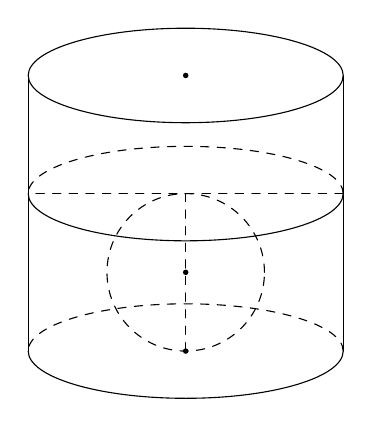
\begin{tikzpicture}[>=stealth,line join=round,line cap=round,font=\footnotesize,scale=1]
			\def\a{2} % ban truc lon = ban kinh tru
			\def\b{0.6} % ban truc nho
			\def\h{3.5} % chieu cao tru
			\path 
			(\a,\h) coordinate (A)
			(\a,0) coordinate (B)
			(0,\h) coordinate (O')
			(0,0) coordinate (O);
			% ve cac canh ben
			\draw (\a,0)--(\a,\h) (-\a,0)--(-\a,\h);
			\fill (O') circle(1pt);
			\fill (O) circle(1pt);
			% mat day giua
			\draw[dashed] (\a,2) arc [x radius=\a, y radius=\b, start angle=0, end angle=180];
			\draw (-\a,2) arc [x radius=\a, y radius=\b, start angle=180, end angle=360];
			% ve day duoi
			\draw[dashed] (\a,0) arc [x radius=\a, y radius=\b, start angle=0, end angle=180];
			\draw (-\a,0) arc [x radius=\a, y radius=\b, start angle=180, end angle=360];
			\draw (0,\h) ellipse (\a cm and \b cm);
			\draw[dashed] (\a,2)--(-\a,2);
			\draw[dashed] (0,1) circle(1);
			\draw[dashed] (0,0)--(0,2);
			\fill (0,1) circle (1pt);
		\end{tikzpicture}
	}
	\loigiai
	{
		\begin{center}
			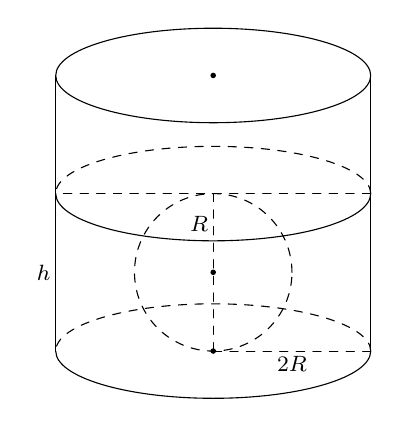
\begin{tikzpicture}[>=stealth,line join=round,line cap=round,font=\footnotesize,scale=1]
				\def\a{2} % ban truc lon = ban kinh tru
				\def\b{0.6} % ban truc nho
				\def\h{3.5} % chieu cao tru
				\path 
				(\a,\h) coordinate (A)
				(\a,0) coordinate (B)
				(0,\h) coordinate (O')
				(0,0) coordinate (O);
				% ve cac canh ben
				\draw (\a,0)--(\a,\h) (-\a,0)--(-\a,\h);
				\draw[dashed] (O)--(B);
				\fill (O') circle(1pt);
				\fill (O) circle(1pt);
				% mat day giua
				\draw[dashed] (\a,2) arc [x radius=\a, y radius=\b, start angle=0, end angle=180];
				\draw (-\a,2) arc [x radius=\a, y radius=\b, start angle=180, end angle=360];
				% ve day duoi
				\draw[dashed] (\a,0) arc [x radius=\a, y radius=\b, start angle=0, end angle=180];
				\draw (-\a,0) arc [x radius=\a, y radius=\b, start angle=180, end angle=360];
				\draw (0,\h) ellipse (\a cm and \b cm);
				\draw[dashed] (\a,2)--(-\a,2);
				\draw[dashed] (0,1) circle(1);
				\draw[dashed] (0,0)--(0,2);
				\fill (0,1) circle (1pt);
				\fill (-\a,1) node[left]{$h$};
				\fill (0,1.62) node[left]{$R$};
				\fill (1,0) node[below]{$2R$};
			\end{tikzpicture}
		\end{center}
		Gọi $r$ là bán kính của viên bi.\\
		Thể tích viên bi là $V_{\textrm{bi}} = \dfrac{4}{3}\pi r^3$.\\
		Phần thể tích nước dâng lên sau khi bỏ viên bi vào là $V_{\textrm{nước}} = \pi\dot (5.4)^2\cdot (2r - 4{,}5)$.\\
		Vì thể tích nước dâng lên chính là thể tích của viên bi nên ta có 
		$$V_{\textrm{bi}} = V_{\textrm{nước}} \Leftrightarrow \dfrac{4}{3}\pi r^3 = \pi\dot (5.4)^2\cdot (2r - 4{,}5) \Leftrightarrow r = 2{,}7 \textrm{ (vì $0 < r < 4{,}5$).} $$
	}
\end{ex}

% #1822 | Archive/2024/San pham - Tex hoa Lop 12 Chuong trinh moi - Dot 5 (Chuong 5)/Data/Chuong 5/Chan troi sang tao/CTST-Chuong5-Bai3-De2.tex | mã gốc 2H5V3-2
\begin{ex}%[2H5V3-2]%[CTST-Chuong5-Bai3-De2]%[Dương Công Tạo]
	 Trong không gian với hệ toạ độ $Oxyz$, cho điểm $A(1;-2;3)$ và $B(3;-2;1)$.
	\choiceTF
	{Mặt cầu $(S)$ đường kính $AB$ có bán kính $R=4$}
	{\True Phương trình mặt cầu $(S)$ đường kính $AB$ là $(S)\colon (x-2)^2+(y+2)^2+(z-2)^2=2$}
	{Mặt cầu $(S)$ đường kính $AB$ tiếp xúc với mặt phẳng $(P)\colon x-y-z+3=0$}
	{Trong không gian $Oxyz$ giả sử một trạm thu phát sóng điện thoại được đặt tại tâm mặt cầu $(S)$ đường kính $AB$ với bán kính phủ sóng bằng bán kính mặt cầu $(S)$ thì người sử dụng điện thoại tại điểm $M(-5;-2;5)$ có thể sử dụng được dịch vụ trạm trên}
	\loigiai{
		\begin{itemchoice}
			\itemch {\bf Sai.}\\
			Mặt cầu $(S)$ đường kính $AB$ có bán kính $R=\dfrac{\sqrt{2^2+0^2+(-2)^2}}{2}=\sqrt{2}$.
			\itemch {\bf Đúng.}\\
			Mặt cầu $(S)$ đường kính $AB$ có \begin{itemize}
				\item Tâm $I(2;0;2)$ là trung điểm của $AB$.
				\item Bán kính $R=\dfrac{\sqrt{2^2+0^2+(-2)^2}}{2}=\sqrt{2}$.
			\end{itemize}
		Do đó có phương trình $(S)\colon(x-2)^2+(y+2)^2+(z-2)^2=2$.
			\itemch {\bf Sai.}\\
			Ta có $\mathrm{d}\big(I;(P)\big)=\dfrac{\left|2-0-2+3\right|}{\sqrt{1^2+1^2+1^2}}=\sqrt{3} > \sqrt{2}$ nên mặt cầu $(S)$ không tiếp xúc với mặt phẳng $(P)$.
			\itemch {\bf Sai.}\\
			Mặt cầu $(S)$ đường kính $AB$ có \begin{itemize}
				\item Tâm $I(2;0;2)$ là trung điểm của $AB$.
				\item Bán kính $R=\dfrac{\sqrt{2^2+0^2+(-2)^2}}{2}=\sqrt{2}$. 
			\end{itemize}
		Do đó có phương trình $(S)\colon(x-2)^2+(y+2)^2+(z-2)^2=2$.\\
		Có $IM=\sqrt{(-5-2)^2+(-2-0)^2+(5-2)^2}=\sqrt{62} > \sqrt{2}$ nên người sử dụng điện thoại tại điểm $M$ không thể sử dụng dịch vụ của trạm.
		\end{itemchoice}
	} 
\end{ex}

% #1843 | Archive/2024/San pham - Tex hoa Lop 12 Chuong trinh moi - Dot 5 (Chuong 5)/Data/Chuong 5/Canh dieu/CD-Chuong5-Ontapchuong-De2.tex | mã gốc 2H5V1-5
\begin{ex}%[2H5V1-5]%[CD - Chương 5 - Ôn tập chương - Đề 2]%[Hector Tran]
	\immini {
		Góc quan sát ngang của một camera là $115^\circ$. Trong không gian $Oxyz$, camera được đặt tại điểm  $C(4; 2; 3)$ và chiếu thẳng về phía mặt phẳng $(P)\colon 2x-y+2z-3=0$. Biết vùng quan sát được trên mặt phẳng $(P)$  của camera là hình tròn. Tính diện tích của vùng quan sát đó\textit{ (làm tròn kết quả đến chữ số thập phân thứ nhất)}.
		\shortans[oly]{69,7}
	}{
		\begin{tikzpicture}[scale=0.6, font=\footnotesize,line join=round, line cap=round, >=stealth]
			\def\a{2}
			\def\b{0.7}
			\def\h{3}
			\path 
			(-1.5,-1) coordinate (P)++(0:\a*3) coordinate (x)	
			($(P)+(60:\a)$) coordinate (y)
			(0,0) coordinate (A)
			($(A)+(2*\a,0)$) coordinate (B)
			($(A)!0.5!(B)$) coordinate (H)
			($(H)+(0,\h)$) coordinate (C)
			;
			\draw(C)--(A) (C)--(B) (x)--(P)--(y);
			\draw[dashed,thin](A)--(B);
			\draw[dashed,thin] (A) arc (180:0:\a cm and \b cm);
			\draw (A) arc (-180:0:\a cm and \b cm);		
			\draw pic["$P$",draw,angle eccentricity=0.5,angle radius=5mm]{angle=x--P--y}
			pic["$115^\circ$",draw,angle eccentricity=1.2,angle radius=5mm]{angle=A--C--B}
			;			
			\path (C)node [scale=1.5]{\faCamera};
		\end{tikzpicture}
	}
	
	\loigiai{
		\begin{center}
			\begin{tikzpicture}[scale=0.8, font=\footnotesize,line join=round, line cap=round, >=stealth]
				\def\a{2}
				\def\b{0.7}
				\def\h{3}
				\path 
				(-1.5,-1) coordinate (P)++(0:\a*3) coordinate (x)	
				($(P)+(60:\a)$) coordinate (y)
				(0,0) coordinate (A)
				($(A)+(2*\a,0)$) coordinate (B)
				($(A)!0.5!(B)$) coordinate (H)
				($(H)+(0,\h)$) coordinate (C)
				;
				\draw(C)--(A) (C)--(B) (x)--(P)--(y);
				\draw[dashed,thin](A)--(B) (C)--(H);
				\draw[dashed,thin] (A) arc (180:0:\a cm and \b cm);
				\draw (A) arc (-180:0:\a cm and \b cm);
				\pic [draw,thin,angle radius=2mm] {right angle = C--H--B};
				\draw pic["$P$",draw,angle eccentricity=0.5,angle radius=5mm]{angle=x--P--y}
				pic["$115^\circ$",draw,angle eccentricity=1.3,angle radius=5mm]{angle=A--C--B}
				;
				\foreach \i/\g in {A/180,B/0,H/-90}
				\fill[black] (\i) circle(1pt)+(\g:3mm)node[scale=1]{$\i$};
				\path (C)node [scale=1.5]{\faCamera}
				(C)circle(1pt)+(90:6mm)node[scale=1]{$C$};
			\end{tikzpicture}
		\end{center}
		Kẻ $CH\perp (P)$, ta có $$CH=\mathrm{d}\left(C;(P)\right)=\dfrac{\left|2\cdot4-1\cdot2+2\cdot3-3\right|}{\sqrt{2^2+(-1)^2+2^2}}=3.$$ 
		Do tam giác $CAB$ cân tại $C$ nên $\widehat{ACH}=57{,}5^\circ$.\\
		Xét tam giác vuông $CAH$ có 
		$$AH=CH\cdot\tan \widehat{ACH}=3\cdot\tan 57{,}5^\circ.$$
		Vậy diện tích của vùng quan sát được của camera là 
		$$S=\pi\cdot r^2=\pi\cdot (3\cdot\tan 57{,}5^\circ)^2\approx 69{,}7 \text { (đvdt).}$$
	}
\end{ex}

% #1846 | Archive/2024/San pham - Tex hoa Lop 12 Chuong trinh moi - Dot 5 (Chuong 5)/Data/Chuong 5/Canh dieu/CD-Chuong5-Ontapchuong-De2.tex | mã gốc 2H5V2-8
\begin{ex}%[2H5V2-8]%[CD - Chương 5 - Ôn tập chương - Đề 2]%[Hector Tran]
	Trong không gian với hệ tọa độ $Oxyz$, một cabin cáp treo xuất phát từ điểm $A(11;4;0)$ và chuyển động đều theo đường cáp có vectơ chỉ phương $\overrightarrow{u}=(-3;-4;0)$ với tốc độ là $5$ m/s (đơn vị trên mỗi trục tọa độ là mét). Giả sử sau $t$ (s) kể từ lúc xuất phát $(t\ge 0)$, cabin đến điểm $M$. Một người đứng tại điểm $O$ quan sát cabin chạy trên cáp treo, sau thời gian bao nhiêu thì khoảng cách giữa người quan sát và cabin gần nhau nhất?
	\shortans[oly]{1,96}
	\loigiai{
		Do tốc độ của cabin là $5$ m/s nên độ dài $AM=\left|\overrightarrow{AM}\right|=5t$ (m).\\ 
		Do hai véc tơ $\overrightarrow{AM}$ và $\overrightarrow{u}$ cùng phương nên $\overrightarrow{AM}=k\cdot\overrightarrow{u}$ với $k$ là số thực dương nào đó.\\ 
		Suy ra $\left|\overrightarrow{AM}\right|=k\left|\overrightarrow{u}\right|=k\sqrt{(-3)^2+(-4)^2+0^2}=5k$.\\
		Suy ra $t=k$, vì thế $\overrightarrow{AM}=k\cdot \overrightarrow{u}=t\overrightarrow{u}=(-3t;-4t;0)$.\\
		Giả sử điểm $M(x;y;z)$ nên $\overrightarrow{AM}=(x-11;y-4;z)$.\\
		Ta có $\heva{&x-11=-3t\\&y-4=-4t\\&z=0}
		\Leftrightarrow \heva{&x=11-3t\\&y=4-4t\\&z=0}$; $t\in \mathbb{R}$ hay $M(11-3t;4-4t;0)$.\\
		Khoảng cách giữa người quan sát và cabin bằng độ dài đoạn
		$$OM=\sqrt{(11-3t)^2+(4-4t)^2+0^2}=\sqrt{25t^2-98t+137}$$
		Khoảng cách gần nhất khi tam thức bậc hai $25t^2-98t+137$ đạt giá trị nhỏ nhất, khi $t=\dfrac{49}{25}=1{,}96$ (s).
	}
\end{ex}

% #1848 | Archive/2024/San pham - Tex hoa Lop 12 Chuong trinh moi - Dot 5 (Chuong 5)/Data/Chuong 5/Canh dieu/CD-Chuong5-Ontapchuong-De2.tex | mã gốc 2H5V3-4
\begin{ex}%[2H5V3-4]%[CD - Chương 5 - Ôn tập chương - Đề 2]%[Hector Tran]
	Trong không gian $Oxyz$ \textit{(đơn vị của các trục tọa độ là km)}, đài kiểm soát không lưu sân bay có tọa độ $(-64;128;64)$. Máy bay bay trong phạm vi cách đài kiểm soát không quá $500$ km thì sẽ hiển thị trên màn hình ra đa. Một máy bay $N$ xuất hiện trên màn hình ra đa và một máy bay $M$ nằm trong mặt phẳng $(P)\colon x-2y+2z-1458=0$ sao cho hai máy bay $M$, $N$ thuộc đường thẳng có vectơ chỉ phương là $\overrightarrow{u}=(1;1;1)$. Khoảng cách nhỏ nhất giữa hai máy bay $M$, $N$ là bao nhiêu km? \textit{(kết quả làm tròn đến hàng đơn vị)}
	\shortans[oly]{260}
	\loigiai{
		Máy bay $N$ xuất hiện trên màn hình ra đa nên $N$ thuộc khối cầu $(S)$ có tâm $I(-64;128;64)$, bán kính $R=500$.\\
		Ta có $\mathrm{d}\left(I,(P)\right)=\dfrac{\left|x_I-2y_I+2z_I-1458\right|}{\sqrt{1^2+2^2+2^2}}=550> R$ nên $(P)$ và $(S)$ không giao nhau.\\
		\begin{center}
			\begin{tikzpicture}[scale=0.8,line join=round, line cap=round,>=stealth]
				\def \d{4}%bán kính
				\def \r{1.25}%bán kính
				\def \t{0.5}	
				\path
				(0,0) coordinate (M)	
				++(0:\d) coordinate (P)	
				(1,3.5) coordinate (I)	
				($(M)!(I)!(P)$) coordinate (H)
				(2,1) coordinate (u)	
				;
				\draw[name path =c1] (I)circle (\r);
				\path[name path=a] (I)--(H);
				\path[name intersections={of=c1 and a}] coordinate (N) at (intersection-1);
				\path ($(N)+(u)-(M)$) coordinate (u')	;
				\draw (-1,0)--(P)
				(N)--(M) (I)--(H)
				;		
				\draw[->](u)--(u');
				\draw pic[draw,angle eccentricity=2,angle radius=3mm]{right angle=P--H--N}
				pic["$\alpha$",draw,angle eccentricity=0.7,angle radius=5mm]{angle=H--M--N}
				;
				\foreach \i/\g in {I/90,N/30,M/-90,H/-90}
				\fill[black] (\i) circle(1pt)+(\g:0.4)node[scale=1]{$\i$};
				\path (P) node[above ] {$(P)$}
				(u)--(u') node[midway,sloped,scale=1,below]{$\overrightarrow {u}$}
				;
			\end{tikzpicture}
		\end{center}
		Gọi $\alpha$ là góc tạo bởi $MN$ và mặt phẳng $(P)$.\\
		Gọi $H$ là hình chiếu của $N$ lên mặt phẳng $(P)$.\\
		Mặt khác $\overrightarrow{MN}$ cùng phương với vectơ $\overrightarrow{u}=(1;1;1)$ và $\overrightarrow{n_P}=(1;-2;2)$\\
		suy ra $\sin \alpha=\dfrac{\left|\overrightarrow{u}\cdot \overrightarrow{n_P}\right|}{\left|\overrightarrow{u}\right|\cdot \left|\overrightarrow{n_P}\right|}=\dfrac{1}{3\sqrt{3}}$.\\
		Khi đó $MN=\dfrac{NH}{\sin \alpha} \ge \dfrac{NH_{\min}}{\sin \alpha}=\dfrac{\mathrm{d}\left(I,(P)\right)-R}{\sin \alpha}=\dfrac{550-500}{\dfrac{1}{3\sqrt{3}}}=150\sqrt{3} \approx 260$. 
	}
\end{ex}

% #1857 | Archive/2024/San pham - Tex hoa Lop 12 Chuong trinh moi - Dot 5 (Chuong 5)/Data/Chuong 5/Canh dieu/CD-Chuong5-Bai2-De2.tex | mã gốc 2H5V2-8
\begin{ex}%[2H5V2-8]%[CD - Chương 5 - Bài 2 - Đề 2]%[Nguyễn Hoài Nam]
Một người đứng ở mặt đất điều khiển flycam để phục vụ chương trình truyền hình. Chọn hệ trục tọa độ $Oxyz$ với gốc tọa độ $O$ là vị trí người điều khiển, mặt phẳng $(Oxy)$ trùng với mặt đất. Chiếc flycam đang ở vị trí $M(1;2;4)$ và chuyển động trên đường thẳng song song với mặt đất. Biết hướng chuyển động của flycam là $\overrightarrow{u}=(a;2;b)$ ($a,b$ là các số nguyên) sao cho khoảng cách từ vị trí người điều khiển đến đường thẳng chuyển động của flycam là bé nhất. Tính $a+b$.
	\shortans{$1$}
	\loigiai{
	\begin{center}
	\begin{tikzpicture}[scale=1, font=\footnotesize, line join=round, line cap=round, >=stealth]
		\path 
			(0,0) coordinate (A)
			(-1,-2) coordinate (B)
			(5,0) coordinate (C)
			($(C)-(A)+(B)$) coordinate (D)
			(2.5,-1) coordinate (O)
			(1,2.5) coordinate (M)
			($(M)+(0.7,-0.1)$) coordinate (K)
			($(O)+(0,2.7)$) coordinate (H)
			($(M)!4!(K)$) coordinate (a)
			($(M)!-0.4!(K)$) coordinate (b);
		\draw (a)--(b);
		\draw (A)--(B)--(D)--(C)--cycle;
		\path (0,3) coordinate (E)
			(-1,1) coordinate (F)
			(5,3) coordinate (P)
			($(P)-(E)+(F)$) coordinate (Q)
			(intersection of M--O and F--Q) coordinate (X)
			(intersection of K--O and F--Q) coordinate (Y)
			(intersection of H--O and F--Q) coordinate (Z);
		\draw (E)--(F)--(Q)--(P)--cycle (X)--(O)--(Y) (Z)--(O) (K)--(H);
		\draw [dashed] (X)--(M) (K)--(Y) (H)--(Z);
		\foreach \i/\j in {M/90, K/90, H/30, O/-90}\draw [fill=black] (\i) circle (1pt) ++(\j:0.3) node {$\i$};
		\draw (a) node [above] {$\Delta$};
		\draw pic[draw, angle radius =1.5mm]{right angle =K--H--O};
		\draw pic[draw, angle radius =1.5mm]{right angle =M--K--O};
		\draw pic[draw,angle radius=1cm] {angle = D--B--A};
		\draw (B) ++(20:0.6) node {\tiny $(Oxy)$}; 
		\draw pic[draw,angle radius=0.7cm] {angle = Q--F--E};
		\draw (F) ++(20:0.4) node {\tiny $(P)$}; 
	\end{tikzpicture}
	\end{center}
	Gọi $(P)$ là mặt phẳng đi qua $M$ và song song với $(Oxy)$, $\Delta$ là đường thẳng mà flycam chuyển động. Khi đó $\Delta$ đi qua $M$ và $(P)$ chứa $\Delta$. \\
	Gọi $H$ là hình chiếu vuông góc của $O$ xuống $(P)$ và $K$ là hình chiếu vuông góc của $O$ xuống $\Delta$.\\
	Vì $OH\leq OK\leq OM$ nên $\mathrm{d}(O,\Delta)$ đạt giá trị nhỏ nhất khi và chỉ khi $OK$ đạt giá trị nhỏ nhất. Khi đó, $K\equiv H$, suy ra $OK\perp (P)$.\\
	Gọi $(Q)$ là mặt phẳng chứa $OK$ và $\Delta$. Khi đó, $(Q)\perp (P)$.\\
	Ta có 
	$$\overrightarrow{u}_{\Delta}=\left[\overrightarrow{n}_{(P)},\overrightarrow{n}_{(Q)}\right]=\left[\vec{n}_{(Oxy)},\overrightarrow{OM}\right]=(1;2;0).$$
	Vậy $a=1$ và $b=0$, nên $a+b=1$.
	}
\end{ex}

% #1863 | Archive/2024/San pham - Tex hoa Lop 12 Chuong trinh moi - Dot 5 (Chuong 5)/Data/Chuong 5/Canh dieu/CD-Chuong5-Ontapchuong-De3.tex | mã gốc 2H5H1-7
\begin{ex}%[2H5H1-7]%[CD - Chương 5 - Bài Ôn tập chương - Đề 3]%[Huỳnh Thanh Chí]
	Trong tiết thể dục học về kĩ thuật chuyền bóng hơi, Nam và An đang tập chuyền bóng cho nhau, Nam ném bóng cho An đỡ, quả bóng bay lên cao nhưng lại lệch sang phải của Nam và rơi xuống vị trí cách An $0{,}5$ m và cách Nam $4{,}5$ m. Biết rằng quỹ đạo của quả bóng nằm trong mặt phẳng $(\alpha)\colon a x+b y+c x+d=0$ và vuông góc với mặt đất. Khi đó giá trị của $a+b+c+d$ bằng (kết quả làm tròn đến đơn vị).
	\shortans{-4}
	
	\begin{center}
		\begin{tikzpicture}[scale=1,font=\footnotesize,line join=round,line cap=round,>=stealth]
			\draw[->] (0,0)--(0,3)node[right]{$z$};
			\draw[->] (0,0)--(4,0)node[above]{$y$};
			\draw[->] (0,0)--(-120:2)node[above]{$x$};
			\fill[red] (70:1) circle (2pt) (-10:3) circle (2pt);
			\fill (0,0) circle (1pt) node[left]{$O$};
			\path (0,0)node[above,inner sep=0pt]{\resizebox{!}{1cm}{\color{gray!50}\faMale}};% Vị trí người đứng Nam
			\path (3.3,0)node[above,inner sep=0pt]{\resizebox{!}{1cm}{\color{gray!50}\faMale}};% Vị trí người đứng
			\draw (-0.5,1.4) node{Nam} (3.4,1.4) node{An};
			\draw[dashed,->] (70:1) arc (140:-15:1.51);
			\draw[dashed] (0,0)--(-10:3)--(3.3,0);
			\path (0,0) coordinate (O)
			(3.3,0) coordinate (A)
			(-10:3) coordinate (B)
			(3.4,0) coordinate (C)
			;
			\draw (-10:1.5)node[below]{$4{,}5$ m} (B)node[right]{$0{,}5$ m};
			\draw pic[draw,angle radius=2mm]{right angle=B--A--C};%Theo chiều dương
		\end{tikzpicture}
	\end{center}
	\loigiai{
		Chọn hệ trục như hình vẽ. Gọi $M$ là điểm mà quả bóng chạm đất.\\
		Khi đó $x_M=0{,}5$, $y_M=\sqrt{4{,}5^2-0{,}5^2}=2\sqrt{5}$.\\
		Vì $(\alpha) \perp(Oxy)$ nên $(\alpha)$ có vectơ chỉ phương $\vec{k}=(0; 0; 1)$.\\
		Mà $(\alpha)$ có vectơ chỉ phương $\overrightarrow{OM}=(0{,}5; 2\sqrt{5}; 0)$.\\
		Khi đó vectơ pháp tuyến của $(\alpha)$ là $\overrightarrow{n}_{(\alpha)}=[\vec{k}, \overrightarrow{OM}]=(-2\sqrt{5}; 0{,}5; 0)$.\\
		Suy ra phương trình mặt phẳng $(\alpha)$ là $(\alpha)\colon -2\sqrt{5} x+0{,}5y=0$.\\
		$\Rightarrow a=-2\sqrt{5}$; $b=0{,}5$; $c=0$; $d=0$ $\Rightarrow a+b+c+d \approx-4$.}
\end{ex}

% #1865 | Archive/2024/San pham - Tex hoa Lop 12 Chuong trinh moi - Dot 5 (Chuong 5)/Data/Chuong 5/Canh dieu/CD-Chuong5-Ontapchuong-De3.tex | mã gốc 2H5V2-8
\begin{ex}%[2H5V2-8]%[CD - Chương 5 - Bài Ôn tập chương - Đề 3]%[Huỳnh Thanh Chí]
	\immini{Trên một sườn núi (có độ nghiêng đều), người ta trồng một cây thông và muốn giữ nó không bị nghiêng bằng hai sợi dây neo như hình vẽ. Giả thiết cây thông mọc thẳng đứng và trong một hệ tọa độ phù hợp, các điểm gốc $O$ (gốc cây thông) và $A, B$ (nơi buộc dây neo) có tọa độ tương ứng là $O(0; 0; 0)$, $A(5;-3; 1)$, $B(-3;-4; 2)$, đơn vị trên mỗi trục tọa độ là mét. Biết rằng hai dây neo đều được buộc vào cây thông tại điểm $C(0; 0; 5)$ và được kéo căng tạo thành các đoạn thẳng. Khi đó, góc tạo bởi dây neo $CA$ và mặt phẳng sườn núi là bao nhiêu độ? (Kết quả làm tròn đến hàng đơn vị của độ).
	\shortans{37}
	}
	{
		\begin{tikzpicture}[line join = round, line cap=round,>=stealth,font=\footnotesize,scale=.7]
			\path 
			(0,0) coordinate (O)
			(-4,0) coordinate (A)
			(-3.5,1.5) coordinate (B)
			(0,2) coordinate (C)
			;
			\tikzset{cucda/.pic={
					\fill[ball color=gray!40!brown](0,0)..controls++(50:2) and++(160:1)..(4,0)..controls++(40:5) and++(130:3)..(10,0)..controls++(-110:2) and++(-140:3)..(0,0);
			}}
			\clip (-5,-1) rectangle (2,5);
			\draw[fill=black!2] (-5,-1) rectangle (2,5);
			
			\draw[fill=black!30] (-5,-1)--(-5,5)--(-4,5)--(2,-1)--cycle;		
			\path ($(B)+(0.5,2)$)pic[scale=0.1,rotate=-45]{cucda}
			($(B)+(2,1)$)pic[scale=0.1,rotate=-45]{cucda}
			($(B)+(3,-1)$)pic[scale=0.1,rotate=-25]{cucda}
			($(B)+(4,-2.5)$)pic[scale=0.1,rotate=0]{cucda}
			($(B)+(2,-2.5)$)pic[scale=0.1,rotate=0]{cucda}
			;			
			\tikzset{thong/.pic={ 
					\fill[green!30] (1,-2)--(-1,-2)--(-1.2,-1)--(-0.8,-1)--(-0.8,-0.2) to [bend left =30] (-3.1,-0.5)--(-2.6,-0.2) to [bend left =15] (-4,0) to [bend right =20] (-2.25,1.25) to [bend left =10] (-3.5,1.4) to [bend right =20] (-1.3,3) to [bend left =15] (-2,2.8)to [bend right =10] (0,5) to [bend right =10] (2,2.2) to [bend left =15] (1.3,3) to [bend right =20] (3.5,1.4) to [bend left =10] (2.25,1.25) to [bend right =20] (4,0) to [bend left =15] (2.6,-0.2) --(3.1,-0.5) to [bend left =30] (0.8,-0.2)--(0.8,-1)--(1.2,-1)--(1,-2);
			}}
			
			
			
			\draw[fill=brown] ($(O)+(0.25,0)$)--(C)--($(O)+(-0.25,0)$)--cycle
			;
			
			\path
			(C)pic[scale=0.2]{thong}
			($(C)+(0,0.5)$)pic[scale=0.2]{thong}
			($(C)+(0,1)$)pic[scale=0.2]{thong}
			($(C)+(0,1.5)$)pic[scale=0.2]{thong}
			;
			\draw[line width=1pt,yellow] (A)--(C)--(B);
			\foreach \p/\r in {A/180,B/90,C/90,O/-90}
			\fill (\p) circle (1.2pt) node[shift={(\r:3mm)}]{$\p$};
			
			\draw[line width=2pt,yellow] pic[draw,angle radius=10mm] { angle = O--A--C}; 
			\draw[line width=2pt,yellow] pic[draw,angle radius=10mm] { angle = O--B--C}; 
			\draw
			($(A)+(0.7,0)$) node[]{$\color{yellow} ?$}
			($(B)+(0.7,-0.2)$) node[]{$\color{yellow} ?$}
			;
		\end{tikzpicture}
	}
		\loigiai{
		Ta có $\overrightarrow{OA}=(5;-3; 1)$, $\overrightarrow{OB}=(-3;-4; 2)$ nên 
		\allowdisplaybreaks
		\begin{eqnarray*}
			\left[\overrightarrow{OA}, \overrightarrow{OB}\right]&=&\left(\left|\begin{array}{cc}-3& 1\\-4& 2\end{array}\right|;\left|\begin{array}{cc}1& 5\\ 2&-3\end{array}\right|;\left|\begin{array}{ll}5&-3\\-3&-4\end{array}\right|\right)\\
			&=&(-2;-13;-11).
		\end{eqnarray*}
		Suy ra vectơ $\vec{n}=\left[\overrightarrow{OA}, \overrightarrow{OB}\right]=(-2;-13;-11)$ là một vectơ pháp tuyến của mặt phẳng $(OAB)$.\\
		Mặt khác $\overrightarrow{CA}=(5;-3;-4)$ nên ta có
		\allowdisplaybreaks
		\begin{eqnarray*}
			\sin \left(CA,(OAB)\right)&=&|\cos (\overrightarrow{CA}, \vec{n})|=\dfrac{|\overrightarrow{CA} \cdot \vec{n}|}{|\overrightarrow{CA}|\cdot|\vec{n}|}\\
			&=&\dfrac{|5\cdot(-2)+(-3) \cdot(-13)+(-4) \cdot(-11)|}{\sqrt{5^2+(-3)^2+(-4)^2} \cdot \sqrt{(-2)^2+(-13)^2+(-11)^2}}\\
			&=&\dfrac{73}{70\sqrt{3}}.
		\end{eqnarray*}
		Suy ra $\left(CA,(OAB)\right) \approx 37^{\circ}$. \\
		Vậy góc tạo bởi dây neo $CA$ và mặt phẳng sườn núi khoảng $37^{\circ}$.
	}
\end{ex}

% #1868 | Archive/2024/San pham - Tex hoa Lop 12 Chuong trinh moi - Dot 5 (Chuong 5)/Data/Chuong 5/Canh dieu/CD-Chuong5-Ontapchuong-De3.tex | mã gốc 2H5V3-4
\begin{ex}%[2H5V3-4]%[CD - Chương 5 - Bài Ôn tập chương - Đề 3]%[Huỳnh Thanh Chí]
	Hệ thống định vị toàn cầu (tên tiếng Anh là: Global Positioning System, viết tắt là GPS) là một hệ thống cho phép xác định chính xác vị trí của một vật thể trong không gian. Ta có thể mô phỏng cơ chế hoạt động của hệ thống GPS trong không gian như sau: Trong cùng một thời điểm, tọa độ của một điểm $M$ trong không gian sẽ được xác định bởi bốn vệ tinh cho trước, trên mỗi vệ tinh có một máy thu tín hiệu. Bằng cách so sánh sự sai lệch về thời gian từ lúc tín hiệu được phát đi với thời gian nhận phản hồi tín hiệu đó, mỗi máy thu tín hiệu xác định được khoảng cách từ vệ tinh đến vị trí $M$ cần tìm toạ độ. Trong không gian với hệ tọa độ $Oxyz$, cho bốn vệ tinh $A(0; 4; 5)$, $B(-3;-1; 3)$, $C(-2; 8; 9)$, $D(-7; 2;-3)$. Tính khoảng cách từ gốc toạ độ $O$ đến điểm $M$ biết rằng khoảng cách từ các vệ tinh đến điểm $M$ lần lượt là $MA=3$, $MB=5$, $MC=9$, $MD=10$. (Kết quả làm tròn đến hàng phần mười).
	\shortans{3{,}7}
	\loigiai{
		\begin{itemize}
			\item $MA=3\Rightarrow$ Điểm $M$ thuộc mặt cầu tâm $A$, bán kính $R=3$ có phương trình $x^2+(y-4)^2+(z-5)^2=9$.
			\item $MB=5\Rightarrow$ Điểm $M$ thuộc mặt cầu tâm $B$, bán kính $R=5$ có phương trình $(x+3)^2+(y+1)^2+(z-3)^2=25$.
			\item $MC=9\Rightarrow$ Điểm $M$ thuộc mặt cầu tâm $C$, bán kính $R=9$ có phương trình $(x+2)^2+(y-8)^2+(z-9)^2=81$.
			\item $MD=10\Rightarrow$ Diểm $M$ thuộc mặt cầu tâm $D$, bán kính $R=10$ có phương trình $(x+7)^2+(y-2)^2+(z+3)^2=100$.
		\end{itemize}
		Ta có $M$ là giao điểm của bốn mặt cầu với tâm lần lượt là bốn vệ tinh $A$, $B$, $C$, $D$.\\
		Toạ độ $M$ là nghiệm của hệ phương trình $\heva{&x^2+(y-4)^2+(z-5)^2=9\\
			&(x+3)^2+(y+1)^2+(z-3)^2=25\\
			&(x+2)^2+(y-8)^2+(z-9)^2=81\\
			&(x+7)^2+(y-2)^2+(z+3)^2=100.}$\\
		Giải hệ phương trình ta được $x=1$, $y=2$, $z=3\Rightarrow M(1; 2; 3)$.\\
		Khoảng cách từ gốc toạ độ $O$ đến điểm $M$ là $OM=\sqrt{1^2+2^2+3^2}=\sqrt{14} \approx 3{,}7$.
	}
\end{ex}

% #1873 | Archive/2024/San pham - Tex hoa Lop 12 Chuong trinh moi - Dot 5 (Chuong 5)/Data/Chuong 5/Canh dieu/CD-Chuong5-Ontapchuong-De1.tex | mã gốc 2H5H1-7
\begin{ex}%[2H5H1-7]%[CD - Chương 5 - Ôn tập chương - Đề 1]%[Lâm Tú]
	Khi gắn hệ trục toạ độ $Oxyz$ (đơn vị trên mỗi trục toạ độ là decimét) vào một ngôi nhà $1$ tầng, người ta thấy rằng mặt trên và mặt dưới của mái nhà thuộc các mặt phẳng vuông góc với trục $Oz$. Biết rằng các vị trí $A(3;4;33), D(9;8;35)$ lần lượt thuộc mặt dưới, mặt trên của mái nhà. Độ dày của mái nhà được tính bằng khoảng cách giữa mặt trên và mặt dưới của mái nhà đó. Hãy cho biết độ dày của mái nhà đó là bao nhiêu decimét?
	\shortans[oly]{2}
	\loigiai{
		Do mặt dưới của mái nhà thuộc mặt phẳng vuông góc với trục $Oz$ và đi qua điểm
		$A\left(3;4;33\right)$ nên phương trình mặt phẳng chứa mặt dưới của mái nhà là
		$$z-33=0.$$
		Khoảng cách từ điểm $D$ đến mặt phẳng chứa mặt dưới của mái nhà bằng
		$$\dfrac{\left| 35-33\right|}{\sqrt{0^2+0^2+1^2}}=2.$$
		Vậy độ dày của mái nhà là $2$ (dm).}
\end{ex}

% #1876 | Archive/2024/San pham - Tex hoa Lop 12 Chuong trinh moi - Dot 5 (Chuong 5)/Data/Chuong 5/Canh dieu/CD-Chuong5-Ontapchuong-De1.tex | mã gốc 2H5V2-8
\begin{ex}%[2H5V2-8]%[CD - Chương 5 - Ôn tập chương - Đề 1]%[Lâm Tú]
	Trên mặt đất phẳng, người ta dựng một cây cột thẳng cao $6$ m vuông góc với mặt đất, có chân cột đặt tại ví trí $\mathrm{O}$ trên mặt đất. Tại một thời điểm, dưới ánh nắng mặt trời, bóng của đỉnh cột dưới mặt đất cách chân cột $3$ m về hướng $S60^\circ$E (hướng tạo với hướng nam góc $60^\circ$ tạo với hướng đông góc $30^\circ$) (như hình vẽ). Chọn hệ trục $\mathrm{Ox}yz$ có gốc tọa độ là $O$, tia $Ox$ chỉ hướng nam, tia $Oy$ chỉ hướng đông, tia $Oz$ chứa cây cột, đơn vị đo là mét. Tính góc tạo bởi đường thẳng chứa tia nắng mặt trời đi qua đỉnh cột tại thời điểm đang xét với mặt đất (kết quả lấy phần nguyên của độ).
	\begin{center}
		\begin{tikzpicture}[scale=1, font=\footnotesize, line join=round, line cap=round, >=stealth]
			\path 
			(0:0) coordinate (O)
			($(O)+(0:3)$) coordinate (y)
			($(O)+(90:3)$) coordinate (z)
			($(O)+(-145:2.5)$) coordinate (x)
			($(O)!1/3!(y)$) coordinate (Y)
			($(O)!1/3!(x)$) coordinate (X)
			($(O)!1/3!(z)$) coordinate (Z)
			($(O)!4/5!(y)$) coordinate (C)
			($(O)!3/5!(x)$) coordinate (B)
			($(O)!3/5!(z)$) coordinate (A)
			($(C)+(B)-(O)$) coordinate (A')
			($(A)+(A')-(O)$) coordinate (M)
			;
			%\draw[dashed] (A)--(a)--(B) (C)--(M)--(a);
			\draw (A')--(O);
			\draw[->] (O)--(y) node[below]{$y$} node[above]{$E$};
			\draw[->] (O)--(z) node[left]{$z$};
			\draw[->] (O)--(x) node[below right]{$x$} node[above left]{$S$};
			\foreach \x/\g in {O/160,A/180,A'/-60}
			\draw[fill=black] 	(\x) circle (.5pt)
			($(\g:.3)+(\x)$) node {$\x$};	
			\shadedraw[inner color=red,outer color=yellow, draw=red] (-2,4) circle(0.4cm);
			\draw pic["$60^\circ$",draw,double,angle eccentricity=1.8,angle radius=3mm]{angle=B--O--A'} pic["$30^\circ$",draw,angle eccentricity=1.8,angle radius=4mm]{angle=A'--O--C};
		\end{tikzpicture}
	\end{center}
	\shortans[oly]{63}
	\loigiai{
		Gọi $A$ (đỉnh cột) và $A'$ (bóng của đỉnh cột).\\
		Ta có $A(0;0;6)$.\\
		Hoành độ của điểm $A'$ là $x=3 \cdot \cos 60^\circ=\dfrac{3}{2}$.\\
		Tung độ của điểm $A'$ là $y=3 \cdot \cos 30^\circ=\dfrac{3\sqrt{3}}{2}$.\\
		Do đó $A'\left(\dfrac{3}{2};\dfrac{3\sqrt{3}}{2};0\right)$.\\
		Đường thẳng chứa tia nắng mặt trời đi qua $A(0;0;6)$ và có vectơ chỉ phương \\ $\overrightarrow{AA'}=\left(\dfrac{3}{2};\dfrac{3\sqrt{3}}{2};-6\right)=\dfrac{3}{2}\left(1;\sqrt{3};-4\right)$.\\
		Phương trình đường thẳng tia nắng có véctơ chỉ phương là $\overrightarrow{u}=\left(1;\sqrt{3};-4\right)$.\\
		Mặt đất là mặt phẳng $\left(Oxy\right)$ có véctơ pháp tuyến là $\overrightarrow{n}=\left(0;0;1\right)$.\\
		Gọi $\alpha $ là góc giữa phương trình đường thẳng tia nắng với mặt phẳng $\left(Oxy\right)$.\\
		Ta có $\sin \alpha 
		=\left| \cos \left(\overrightarrow{u};\overrightarrow{n}\right)\right|
		=\dfrac{\left| \overrightarrow{u} \cdot \overrightarrow{n}\right|}
		{\left| \overrightarrow{u}\right| \cdot \left| \overrightarrow{n}\right|}
		=\dfrac{\left| -4\right|}{\sqrt{1+3+16} \cdot \sqrt{1}}=\dfrac{2}{\sqrt{5}}$.\\
		$\Leftrightarrow \alpha \approx{63^\circ}26'$.}
\end{ex}

% #1887 | Archive/2024/San pham - Tex hoa Lop 12 Chuong trinh moi - Dot 5 (Chuong 5)/Data/Chuong 5/Canh dieu/CD-Chuong5-Bai1-De1.tex | mã gốc 2H5V1-7
\begin{ex}%[Cánh Diều - Chương 5 - Bài 1 - Đề 1]%[Nguyễn Tài Tuệ]%[2H5V1-7]
	Trong một trò chợi mô phỏng bắn súng, một người chơi đặt điểm ngắm tại điểm $O$ là giao điểm của $AC$ và $BD$ trong căn phòng hình hộp chữ nhật $ABCD\cdot A'B'C'D'$ có kích thước $AB=50$ (m), $AD=35$ (m), $AA'=10$ (m). Người chơi có nhiệm vụ từ điểm ngắm đã đặt bắn trúng một mục tiêu đi động trên mặt phẳng $\left(CB'D'\right)$. Tính khoảng cách ngắn nhất từ điểm ngắm đó đến mục tiêu (làm tròn đến chữ số thập phân thứ $2$).	
	\shortans{$9,44$} 
	\loigiai{	
		\begin{center}
			\begin{tikzpicture}[scale=1,line cap=round,line join=round,font=\footnotesize,>=stealth,declare function={c=0.65;kc=0.15;cao=6*c+3*kc;dai=1.65*cao;dait=dai/3;}]
				\path
				(0,0) coordinate (A)
				($(A)+(-150:1.5)$) coordinate (D)
				($(D)+(0:3)$) coordinate (C)
				($(A)+(0:3)$) coordinate (B)
				($(A)+(90:3)$) coordinate (A')
				($(B)+(90:3)$) coordinate (B')
				($(C)+(90:3)$) coordinate (C')
				($(D)+(90:3)$) coordinate (D')
				($(B)+(0:1)$) coordinate (y)
				($(D)+(-150:1)$)  coordinate (x)
				($(A')+(90:1)$) coordinate (z)
				($(B)!0.5!(D)$) coordinate (O)
				;
				\draw (A')--(B')--(C')--(D')--(A') (B')--(B)--(C)--(D)--(D') (C)--(C') (C)--(B')--(D')--(C);
				\draw[->] (D)--(x)node[shift=(-90:0.5)]{$x$};
				\draw[->] (B)--(y)node[shift=(-90:0.5)]{$y$};
				\draw[->] (A')--(z)node[shift=(-180:0.5)]{$z$};
				\draw[dashed]  (A)--(A') (D)--(B)--(A)--(D);
				\foreach \p/\r in {A/-90, B/-90, C/-90,D/-90,A'/40,D'/90,B'/90,C'/-20,O/-90}
				\fill (\p) circle (1.25pt) node[shift={(\r:3mm)}]{$\p$};
			\end{tikzpicture}
		\end{center}
		\noindent	
		Chọn hệ trục tọa độ như hình vẽ, ta có $B'(50; 0; 10), D'(0; 35; 10), C(50; 35,0)$ và $O(25; 17,5; 0)$.\\
		Mặt phẳng $\left(CB'D'\right)$ nhận $\overrightarrow{B'D'}=(-50; 35; 0)$ và $\overrightarrow{CB'}=(0;-35; 10)$ làm cặp vectơ chỉ phương nên $(CBD)$ nhận $\vec{n}=[\overrightarrow{BD},\overrightarrow{CB}]=(350; 500; 1750)$ làm vectơ pháp tuyến.\\		
		Mặt khác, $\left(CB'D'\right)$ qua $D'(0; 35; 10)$ nên có phương trình $35x+50y+175z-3500=0$.\\
		Do mục tiêu di động trên mặt phẳng $\left(C'BD\right)$ nên khoảng cách ngắn nhất từ điểm ngắm đến mục tiêu chính là khoảng cách từ điểm $O$ đến mặt phẳng $\left(C'BD\right)$.\\
		Ta có $\mathrm{d}\left(O;\left(C'BD\right)\right)=\dfrac{|35\cdot 25+50\cdot 17,5+75\cdot 0-3500|}{\sqrt{35^2+50^2+175^2}}\approx 9,44(\mathrm{~m})$.\\
		Vậy khoảng cách ngắn nhất từ điểm ngắm đến mục tiêu là khoảng $9,44$ mét.
	}
\end{ex}

% #1893 | Archive/2024/San pham - Tex hoa Lop 12 Chuong trinh moi - Dot 5 (Chuong 5)/Data/Chuong 5/Canh dieu/CD-Chuong5-Bai1-De2.tex | mã gốc 2H5V1-7
\begin{ex}%[2H5V1-7]%[CD - Chương 5 - Bài 1 - Đề 2]%[Đoàn Thị Lý]
	Hình vẽ dưới đây minh họa hình ảnh hai mái nhà của một nhà kho trong không gian với hệ tọa độ $Oxyz$ (đơn vị trên mỗi trục tọa độ là mét).
	\begin{center}
		\begin{tikzpicture}[scale=1, font=\footnotesize, line join=round, line cap=round, >=stealth]
			\path
			(0:0) coordinate (y)--++(-35:1) coordinate (Y)--++(-35:3) coordinate (O)--++(20:5) coordinate (X)--++(145:3)coordinate (T)
			--++(90:4) coordinate (B) (Y)--++(90:4)coordinate (C) (O)--++(90:2)coordinate (D)--++(90:5)coordinate (z) (X)--++(90:2)coordinate (A)--++(-145:2.5)coordinate (P)--++(125:4.2)coordinate (Q)
			(X)--++(20:1)coordinate (x)
			;
			\foreach \x/\g in {O/-90,A/0,P/-90,C/180,D/-140,B/0,Q/0}
			\fill[black](\x) circle (1pt)
			($(\x)+(\g:3mm)$);
			\draw[dashed] (X)--(T)--(Y) (T)--(B);
			\draw[->] (O)--(x) node[below]{$x$};
			\draw[->] (O)--(y) node[below]{$y$};
			\draw[->] (O)node[below]{$O$}--(z) node[left]{$z$};
			\draw (Y)--(C)node[left]{$C(0;8;20)$}--(Q)node[right]{$Q$}--(B)node[right]{$B(12;8;20)$}--(A)node[right]{$A(12;0;10)$}--(X) (A)--(P)node[below]{$P(6;0;4)$}--(D)node[below left]{$D(0;0;10)$}--(C) (P)--(Q);
		\end{tikzpicture}
	\end{center}
	Các bức tường của nhà kho đều được xây vuông góc với mặt đất. Biết tọa độ vectơ $\overrightarrow{PQ}=(x;y;z)$, tính $x+y+z$.
	\shortans{$18$}
	\loigiai{
		Hai mặt phẳng tương ứng mỗi mái nhà là $(ABP)$ và $(CDP)$.\\
		Do $(ABP)$ có cặp vectơ chỉ phương là $\overrightarrow{AB}=(0;8;1$), $\overrightarrow{AP}=(-6;0;-6)$, suy ra $(ABP)$ có vectơ pháp tuyến là $\left[ \overrightarrow{AB}, \overrightarrow{AP}\right] =(-48 ;-60 ;48)$.\\
		Mà $(ABP)$ đi qua $P(6;0;4)$ suy ra \[(ABP)\colon -48(x-6)-60(y-0)+48(z-6)=0
		\Leftrightarrow 4 x+5 y-4 z-8=0.\]
		Do $(CDP)$ có cặp vectơ chỉ phương là $\overrightarrow{DP}=(6;0;-6)$, $\overrightarrow{DC}=(0;8;10)$ suy ra $(CDP)$ có vectơ pháp tuyến là $\left[ \overrightarrow{DP}, \overrightarrow{DC}\right] =(48 ;-60 ; 48)$.\\
		Mà $(CDP)$ đi qua $P(6;0;4)$ suy ra \[(CDP)\colon 48(x-6)-60(y-0)+48(z-4)=0
		\Leftrightarrow 4 x-5 y+4 z-40=0.\]
		Vì các bức tường của nhà kho đều được xây vuông góc với mặt đất nên với hệ tọa độ trên, ta có $(CBQ)\colon y-8=0$.\\
		Ta thấy $Q$ thuộc cả $3$ mặt phẳng $(ABP)$, $(CDP)$ và $(CBQ)$ nên tọa độ $Q$ là nghiệm của hệ phương trình
		\[\heva{&4x+5y-4z-8=0\\&4x-5y+4z-40=0\\&y-8=0} \Leftrightarrow \heva{&x=6 \\&	y=8 \\&	z=14} \Rightarrow Q(6;8;14) \Rightarrow \overrightarrow{PQ}=(0;8;10).\] Vậy  $x+y+z=18$.
	}
\end{ex}

% #1894 | Archive/2024/San pham - Tex hoa Lop 12 Chuong trinh moi - Dot 5 (Chuong 5)/Data/Chuong 5/Canh dieu/CD-Chuong5-Bai1-De2.tex | mã gốc 2H5V1-7
\begin{ex}%[2H5V1-7]%[CD - Chương 5 - Bài 1 - Đề 2]%[Đoàn Thị Lý] 
	Hai đứa trẻ đang chơi với một quả bóng. Bé gái ném quả bóng cho bé trai. Quả bóng di chuyển trong không khí, uốn cong $3$ m về bên phải và rơi cách bé gái $5$ m. Chọn hệ trục toạ độ như hình vẽ sau.
	\begin{center}
		\begin{tikzpicture}[scale=1, font=\footnotesize, line join=round, line cap=round, >=stealth]
			\path
			(0:0) coordinate (x)--++(80:3) coordinate (B)--++(0:5) coordinate (C)--++(0:1) coordinate (D)
			(C)--++(-100:2)coordinate (E)--++(150:5)coordinate (F)
			(B)--++(90:2) coordinate (z);
			\draw[gray] ($(C)!.08!(B)$) coordinate (X) ($(C)!.15!(E)$) coordinate (Y) (X)--($(X)+(Y)-(C)$)-- (Y);
			\draw ($(C)!.5!(E)$) node[right]{$3$ m};
			\draw ($(B)!.5!(E)$) node[below left]{$5$ m};
			\draw (E) .. controls (2,4) .. (F);
			\draw[dashed] (B)node[below left]{$O(0;0;0)$}--(E)--(C)node[above]{$C$};
			\draw[->](B)--(x)node[left]{$x$};
			\draw[->](B)--(z)node[left]{$z$};	
			\draw[->](B)--(D)node[above]{$y$};
			\fill[blue] (1.6,3.7) circle (.3); 
			\fill[brown] (B)node[above left]{Bé gái} circle (.1); 
			\fill[brown] (C)node[below right]{Bé trai} circle (.1); 
		\end{tikzpicture}
	\end{center}
	Biết mặt phẳng chứa quỹ đạo của quả bóng vuông góc với mặt đất và phương trình tổng quát của nó có dạng $x+by+c=0$. Tính $b+c$ (kết quả làm tròn đến hàng phần chục).
	\shortans{$-0{,}8$}
	\loigiai{
		Ta có $OC=\sqrt{OB^2-BC^2}=4$ suy ra $B(3;4;0)$.\\
		Mặt phẳng chứa quỹ đạo đi qua $O(0;0;0)$ và nhận $\overrightarrow{k}=(0;0;1)$, $\overrightarrow{OB}=(3;4;0)$ làm vectơ chỉ phương.\\
		Suy ra vectơ pháp tuyến $\overrightarrow{n}=\left[ \overrightarrow{k},\overrightarrow{OB}\right] =(-4;3;0)$.\\
		Vậy phương trình mặt phẳng chứa quỹ đạo của quả bóng là 
		\[-4(x-0)+3(y-0)+0(z-0)=0\Leftrightarrow 4 x-3 y=0\Leftrightarrow x-\dfrac{3}{4}y=0.\]
		Vậy $b+c=-\dfrac{3}{4}\approx -0{,}8$.
	}
\end{ex}

% #1896 | Archive/2024/San pham - Tex hoa Lop 12 Chuong trinh moi - Dot 5 (Chuong 5)/Data/Chuong 5/Canh dieu/CD-Chuong5-Bai1-De2.tex | mã gốc 2H5V1-7
\begin{ex}%[2H5V1-7]%[CD - Chương 5 - Bài 1 - Đề 2]%[Đoàn Thị Lý]
	Một nhà hàng được xây dựng theo mô hình là hình chóp cụt $OAGD.BCFE$ có hai đáy song song với nhau. Mặt sân $OAGD$ là hình chữ nhật và được gắn hệ trục $Oxyz$ như hình vẽ dưới (đơn vị trên mỗi trục tọa độ là mét). 
	\begin{center}
		\begin{tikzpicture}[scale=1, font=\footnotesize, line join=round, line cap=round, >=stealth]
			\path
			(0:0) coordinate (y)--++(-35:1) coordinate (D)--++(-35:3) coordinate (O)--++(20:5) coordinate (A)--++(145:3)coordinate (G)
			--++(120:2.5) coordinate (F)--++(-160:2)coordinate (E)--++(-35:2.5)coordinate (B)--++(20:2)coordinate (C) 
			(O)--++(90:6) coordinate (z)
			(A)--++(20:1)coordinate (x)
			;
			\foreach \x/\g in {O/-90,A/-90,B/80,C/20,D/200,E/180,F/50,G/-100}
			\fill[black](\x) circle (1pt)
			($(\x)+(\g:3mm)$) node{$\x$};
			\draw[dashed] (D)--(G)--(A) (G)--(F);
			\draw[->] (O)--(x) node[below]{$x$};
			\draw[->] (O)--(y) node[below]{$y$};
			\draw[->] (O)node[below]{$O$}--(z) node[left]{$z$};
			\draw (D)--(E)--(F)--(C)--(B)--(E) (B)--(O) (C)--(A);
		\end{tikzpicture}
	\end{center}
	Mặt sân $OAGD$ có chiều dài $OA=100 \mathrm{~m}$, chiều rộng $OD=60$ m và tọa độ điểm $B(10;10;8)$.
	Khoảng cách từ điểm $G$ đến mặt phẳng $(OBED)$ là bao nhiêu mét (kết quả làm tròn đến hàng phần chục)?
	\shortans{$62{,}5$}
	\loigiai{
		Ta có $\overrightarrow{OD}=(0;60;0)$, $\overrightarrow{OB}=(10;10;8)$.\\
		Vectơ pháp tuyến của mặt phẳng $(OBED)$ là $\overrightarrow{n}=\left[\overrightarrow{OD},\overrightarrow{OB}\right] =(480;0;-600)$.\\
		Phương trình mặt phẳng $(OBED)$ đi qua điểm $O(0;0;0)$ và có vectơ pháp tuyến $\overrightarrow{n}_1=(4;0;-5)$ là $4 x-5 z=0$.\\
		Khoảng cách từ điểm $G$ đến mặt phẳng $(OBED)$ là
		\[\mathrm{d}\left(G,(OBED)\right) =\dfrac{|4\cdot 100-5\cdot 0|}{\sqrt{16+25}}=\dfrac{400 \sqrt{41}}{41} \approx 62{,}5 \mathrm{~m}.\]
	}
\end{ex}

% #3155 | Archive/2024/TaiLieuGiangDay/5.HH Oxyz/VDC_TDM.tex | mã gốc 2H5C3-4
\begin{ex}%[2H5C3-4]
	Trong không gian $Oxyz$, tỉ lệ dài trên các trục là $10$ km tính cho một đơn vị tỉ lệ trên mỗi trục, cho bốn vệ tinh có toạ độ lần lượt là $A(-1;2;-1)$, $B(1;4;0)$, $C(3;0;9)$, $D(7;10;-1)$. Đang tiến hành theo dõi vật thể $ M $ (coi là một chất điểm). Ở một thời điểm cả 4 vệ tinh bắn tín hiệu về $M$ và đo được $MA = 6$, $MB = 3$, $MC = 10$, $MD = 6$. Ngay sau đó $10$ giây cả $4$ vệ tinh lại bắn tín hiệu về vật $ M $ và đo được $ MA = 3 $, $ MB = 4 $, $ MC = \sqrt{85} $, $ MD = \sqrt{137} $. Nếu coi như vật $ M $ chuyển động thẳng đều thì tốc độ của vật $ M $ bằng bao nhiêu km/s? (Kết quả làm tròn đến hai chữ số thập phân).
	\shortans[oly]{$0{,}64$}
	\loigiai
	{
	Đặt $M_1(x_1;y_1;z_1)$ là tọa độ vật thể $M$ ở thời điểm ban đầu. \\
	Ta có 
	$\heva{&M_1A=6\\&M_1B=3\\&M_1C=10\\&M_1D=6}$ $\Leftrightarrow$  	$\heva{&M_1A^2=36\\&M_1B^2=9\\&M_1C^2=100\\&M_1D^2=36}$$\Leftrightarrow$  
	$\heva{&(x_1 + 1)^2 + (y_1 - 2)^2 + (z_1 + 1)^2 = 36 \\&(x_1 - 1)^2 + (y_1 - 4)^2 + z_1^2 = 9\\&(x_1 - 3)^2 + y_1^2 + (z_1 - 9)^2 = 100 \\&(x_1 - 7)^2 + (y_1 - 10)^2 + (z_1 + 1)^2 = 36 }$\\	$\Leftrightarrow$ $\heva{&x_1^2+y_1^2+z_1^2+2x_1-4y_1+2z_1=30\quad (1)\\&x_1^2+y_1^2+z_1^2-2x_1-8y_1=-8 \quad (2)\\&x_1^2+y_1^2+z_1^2-6x_1-18z_1=10\quad (3)\\&x_1^2+y_1^2+z_1^2-14x_1-20y_1+2z_1=-114\quad (4)}$$\Rightarrow$ $\heva{&4x_1 + 4y_1 + 2z_1 = 38  \quad \text{(lấy(1)-(2))} \\&8x_1-4y_1+20z_1=20\quad \text{(lấy(1)-(3))}\\&16x_1 + 16y_1 = 144\quad \text{(lấy(1)-(4))}}$\\
	Giải hệ phương trình ta được  $\heva{&x_1=3\\&y_1=6\\&z_1=1}$. Vậy $M_1(3;6;1)$. 
	Tương tự đặt $M_2(x_2;y_2;z_2)$ là tọa độ vật thể $M$ ở thời điểm $t=10 $ giây. \\
	Ta có 
	$\heva{&M_2A=3\\&M_2B=4\\&M_2C=\sqrt{85}\\&M_2D=\sqrt{137}}$ $\Leftrightarrow$  	$\heva{&M_2A^2=9\\&M_2B^2=16\\&M_2C^2=85\\&M_2D^2=137}$$\Leftrightarrow$  
	$\heva{&(x_2 + 1)^2 + (y_2 - 2)^2 + (z_2 + 1)^2 = 9 \\&(x_2 - 1)^2 + (y_2 - 4)^2 + z_2^2 = 16\\&(x_2 - 3)^2 + y_2^2 + (z_2 - 9)^2 = 85 \\&(x_2 - 7)^2 + (y_2 - 10)^2 + (z_2 + 1)^2 = 137 }$\\	$\Leftrightarrow$ $\heva{&x_2^2+y_2^2+z_2^2+2x_2-4y_2+2z_2=3\quad (5)\\&x_2^2+y_2^2+z_2^2-2x_2-8y_2=-1 \quad (6)\\&x_2^2+y_2^2+z_2^2-6x_2-18z_2=-5\quad (7)\\&x_2^2+y_2^2+z_2^2-14x_2-20y_2+2z_2=-13\quad (8)}$$\Rightarrow$ $\heva{&4x_2 + 4y_2 + 2z_2 = 4  \quad \text{(lấy(5)-(6))} \\&8x_2-4y_2+20z_2=8\quad \text{(lấy(5)-(7))}\\&16x_2 + 16y_2 = 16\quad \text{(lấy(5)-(8))}}$\\
	Giải hệ phương trình ta được $\heva{&x_2=1\\&y_2=0\\&z_2=0}$. Vậy $M_2(1;0;0)$. \\
	Quãng đường vật thể $M$ di chuyển là $M_1M_2=\sqrt{41}$.\\ Tốc độ của vật thể $M$ là $v=\dfrac{M_1M_2}{t}=\dfrac{\sqrt{41}}{10}\approx 0{,}64$ km/s.
	}
\end{ex}

% #3499 | Archive/2024/San pham - To Latex Strong - Tex hoa Lop 12 moi - Dot 3 (Chuong 1 + 2 +3 + 4)/Data/Chuong 2/Chan troi sang tao/To 3 - Dot 17 - Chuong 2 - Bai 3 - CTST - De 2.tex | mã gốc 2H5V1-5
\begin{ex}%[2H5V1-5]%[Tổ 3 - Đợt 17 - Chương 2 - Bài 3 - CTST - Đề 2]%[Sauluoi3105]
	\immini{
		Một sân vận động được xây dựng theo mô hình là hình chóp cụt $OAGD.BCFE$ có hai đáy song song với nhau. Mặt sân $OAGD$ là hình chữ nhật và được gắn hệ trục $O x y z$ như hình vẽ dưới (đơn vị trên mỗi trục tọa độ là mét). Mặt sân $OAGD$ có chiều dài $O A=100 \mathrm{~m}$, chiều rộng $OD=60 \mathrm{~m}$ và tọa độ điểm $B(10 ; 10 ; 8)$. Tính khoảng cách từ điểm $G$ đến mặt phẳng $(OBED)$.
	}{
		\begin{tikzpicture}[scale=.85,font=\footnotesize, line join=round, line cap=round, >=stealth]
			\coordinate[label=below:$O$] (O) at (0,0);
			\coordinate[label=below:$A$] (A) at (30:3);
			\coordinate[label=below:$D$] (D) at (170:3);
			\coordinate [label=below:$G$] (G) at ($(A)+(D)-(O)$);
			\coordinate[label=right:$B$] (B) at (70:2.5);
			\coordinate [label=right:$C$] (C) at ($0.8*(A)-0.8*(O)+(B)$);
			\coordinate [label=above:$F$] (F) at ($0.8*(G)-0.8*(A)+(C)$);
			\coordinate [label=above left:$E$] (E) at ($0.8*(D)-0.8*(G)+(F)$);
			\draw[dashed] (D)--(G)--(F) (G)--(A);
			\draw[->] (O)--($1.2*(A)-1.2*(O)$) node[below]{$x$};
			\draw[->] (O)--($1.2*(D)-1.2*(O)$)node[below]{$y$};
			\draw[->] (O)--($1.2*(90:3.5)-1.2*(O)$)node[left]{$z$};
			\draw (O)--(B)--(C)--(A)  (D)--(E)--(F)--(C) (E)--(B);
			\fill (O) circle(1.5pt) (A) circle(1.5pt) (D) circle(1.5pt) (G)circle(1.5pt) (B)circle(1.5pt);
		\end{tikzpicture}
	}
	\shortans{$62{,}5 \mathrm{~m}$}
	\loigiai{
		Ta có $A(100 ; 0 ; 0)$; $D(0;60;0) \Rightarrow G(100 ; 60 ; 0);\overrightarrow{O D}=(0 ; 60 ; 0)$;\\
		Điểm $B(10 ; 10 ; 8) \Rightarrow \overrightarrow{O B}=(10 ; 10 ; 8)$.\\
		Vectơ pháp tuyến của mặt phẳng $(O B E D)$ là $\vec{n}=[\overrightarrow{O D}, \overrightarrow{O B}]=(480 ; 0 ;-600)=120(4 ; 0 ;-5)$.\\
		Phương trình mặt phẳng $(O B E D)$ đi qua điểm $O(0 ; 0 ; 0)$ và có vectơ pháp tuyến $\vec{n}=(4 ; 0 ;-5)$ là: $4 x-5 z=0$\\
		Khoảng cách từ điểm $G$ đến mặt phẳng $(O B E D)$ là
		$$\mathrm{d}\,(G,(O B E D))=\dfrac{|4\cdot 100-5\cdot 0|}{\sqrt{16+25}}=\dfrac{400 \sqrt{41}}{41} \approx 62{,}5\,(\mathrm{m}).$$
	}
\end{ex}

% #3827 | Archive/SP_KhoLatex/SP_Đề Theo Bài-Khối 12/2-OTC5-De2.tex | mã gốc 2H5C3-4
\begin{ex}%[2H5C3-4]
	Một nguồn âm phát ra sóng âm là sóng cầu. Khi gắn hệ trục tọa độ $O x y z$ (đơn vị trên mỗi trục là mét). Cường độ âm chuẩn tại điểm $I(3 ; 4 ; 5)$ là tâm của nguồn phát âm với bán kính $10 \mathrm{~m}$. Để kiểm tra một điểm ở vị trí $M(7 ; 10 ; 17)$ có nhận được cường độ âm phát ra tại $I$ hay không người ta sẽ tính khoảng cách giữa hai vị trí $I$ và $M$. Hỏi khoảng cách giữa hai vị trí $I$ và $M$ là bao nhiêu mét?
	\shortans{$14$}
	\loigiai{
	Ta có $IM=\sqrt{(7-3)^2+(10-4)^2+(17-5)^2}=14m$.
	}
\end{ex}

% #4000 | Archive/SP_KhoLatex/SP_Đề Theo Bài-Khối 12/2-OTCK2-De3.tex | mã gốc 2H5C3-4
\begin{ex}%[2H5C3-4]
	Trong không gian với hệ tọa độ $Oxyz$, đài kiểm soát không lưu sân bay có tọa độ $O(0;0;0)$, mỗi đơn vị trên trục ứng với $1$ km. Máy bay bay trong phạm vi cách đài kiểm soát $417$ km sẽ hiển thị trên màn hình ra đa. Một máy bay đang ở vị trí $A\left(-688;-185;8\right)$, chuyển động theo đường thẳng $d$ có véc-tơ chỉ phương là $\vec{u}=(91;75;0)$ và hướng về đài kiểm soát không lưu.
	\begin{center}
		\begin{tikzpicture}
			\def\r{3}
			\def \x{3}  %bán kính trục lớn elip
			\def \y{1.2} 
			\coordinate (o1) at (-\r,0);
			\coordinate (o2) at (\r,0);
			\coordinate (O) at (0,0);
			
			% ve mp
			\coordinate (P) at (-5,2);
			\coordinate (Q) at ($(P)+(240:6)$);
			\coordinate (R) at ($(Q)+(12,0)$);
			\coordinate (S) at ($(R)+(60:6)$);
			\fill[cyan!20] (P)--(Q)--(R)--(S)--cycle;
			
			
			\draw (O) circle(\r); 
			\path[fill=orange!20] (O) circle(\r); 
			\fill[orange!80] (o2) arc (0:-180:\x cm and \y cm) arc (180:360:\x cm and \x cm);
			\draw[dashed] (o2) arc (0:180:\x cm and \y cm);
			\draw (o2) arc (0:-180:\x cm and \y cm);
			
			% truc oz
			\coordinate (Oz) at (0,4.5);
			\coordinate (Oz') at (0,2.5);
			\coordinate (Oz'') at (0,-3.5);
			\draw[dashed] (Oz'')--(Oz');
			\draw[->] (Oz')--(Oz);
			% tru  ox
			\def\t{240}
			\coordinate (Ox) at ({\x*cos(\t)},{\y*sin(\t)});
			\coordinate (Ox') at ($(O)!2!(Ox)$);
			\coordinate (Ox'') at ($(Ox)!2.2!(O)$);
			\draw[dashed] (O)--(Ox);
			\draw[->] (Ox)--(Ox');
			\draw[dashed] (O)--(Ox'');
			% truc oy
			\coordinate (O4) at (\r,0);
			\coordinate (O5) at (1.5*\r,0);
			\coordinate (O2) at (-\r,0);
			\coordinate (O1) at (-1.5*\r,0);
			\draw (O1)--(O2);
			\draw[dashed] (O2)--(O4);
			\draw[->] (O4)--(O5);
			% duong d
			\coordinate (A) at (-4.52,1.7);
			\coordinate (A3) at (4.5,0.3);
			\coordinate (A1) at ($(A)!0.25!(A3)$);
			\coordinate (A2) at ($(A)!0.82!(A3)$);
			\draw (A)--(A1);
			\draw[dashed] (A1)--(A2);
			\draw (A2)--(A3);
			\foreach \x in {O}{
				\fill (\x) circle(1pt);
			}
			\path 
			node at (O) [above left]{$O$}
			node at (A) [above] {$A$}
			node at (A1) [above]{B}
			node at (A2) [above right]{$C$}
			node at (A3) [above]{$d$}
			node at (Oz) [left]{$z$}
			node at (O5) [below]{$y$}
			node at (Ox')[below]{$x$}
			;
		\end{tikzpicture}
	\end{center}		
	Máy bay bay gần đài kiểm soát không lưu nhất ở vị trí $K(a;b;c)$. Khi đó $a+b+c$ bằng bao nhiêu?
	\shortans{$48$}		
	\loigiai{
		Gọi $(P)$ là mặt phẳng đi qua $O$ và vuông góc với đường thẳng $d$. \\
		Ta có $(P) \perp d$ nên nhận véc-tơ chỉ phương của $d$ là một véc-tơ pháp tuyến.\\
		Vậy $(P)$ đi qua $O(0;0;0)$ và có véc-tơ pháp tuyến $\vec{n}_{P}=\vec{u}_d=(91;75;0)$ nên có phương trình $91\cdot (x-0)+75\cdot (y-0)+0\cdot (z-0)=0 \Leftrightarrow 91x+75y=0$.\\
		Gọi $K$ là hình chiếu vuông góc của $O$ lên đường thẳng $d$, ta có $K$ là giao của đường thẳng $d$ và mặt phẳng $(P)$. Khi đó tọa độ của $K$ là nghiệm của hệ phương trình 
		\begin{eqnarray*}
			\heva{&x=-688 +91t \\ &y=-185+75t\\ &z=8 \\& 91x+75y=0} 
			\Leftrightarrow
			\heva{&x=-688 +91t \\ &y=-185+75t\\ &z=8 \\& 91 \cdot(-688 +91t)+75 \cdot (-185+75t)=0}  
			\Leftrightarrow \heva{& t=\dfrac{11}{2} \\& x=-\dfrac{375}{2}\\&y=\dfrac{455}{2}\\&z=8.}
		\end{eqnarray*}
		Vậy $K\left(-\dfrac{375}{2};\dfrac{455}{2};8\right)$. Tọa độ của vị trí mà máy bay bay gần đài kiểm soát không lưu nhất chính là $K\left(-\dfrac{375}{2};\dfrac{455}{2};8\right)$.\\						
	}
\end{ex}

% #4088 | Archive/SP_KhoLatex/SP_Đề Theo Bài-Khối 12/2-B14-De2.tex | mã gốc 2H5V1-4
\begin{ex}%[2H5V1-4]
Trong không gian $Oxyz$, cho $(\alpha) \colon y+2z-4=0$, $(\beta) \colon  x + y -z +3 =0$, $(\gamma) \colon x+y+z-2=0$. Phương trình mặt phẳng $(P)$ qua giao tuyến hai mặt phẳng $(\alpha)$ và $(\beta)$, đồng thời $(P)$ vuông góc với mặt phẳng $(\gamma)$ có dạng $ax+by+cz+13=0$. Giá trị $a+b+c$ bằng bao nhiêu?  
\shortans{$0$}
\loigiai{
Phương trình $(P) \colon  m(y+2z-4) + n(x+y-z+3) = 0$ với $m^2 + n^2  \ne 0$.\\
Hay $(P) \colon nx + (m+n)y + (2m-n)z -4m+3n = 0.$\\
Vectơ pháp tuyến của $(\alpha)$, $(\beta)$, $(\gamma)$ lần lượt là $\vec{n}_{(\alpha)} = (0;1;2)$, $\vec{n}_{(\beta)}=(1;1;-1)$, $\vec{n}_{(\gamma)} = (1;1;1)$.\\
Do $(P)$ qua giao tuyến của $(\alpha)$ và $(\beta)$ nên 
$\vec{a}_{1}=\left[\vec{n}_{(\alpha)},\vec{n}_{(\beta)}\right] = (-3;2;-1)$ là một vectơ chỉ phương của $(P)$.\\
Do $(P) \perp (\gamma)$ nên $\vec{a}_{2} = \vec{n}_{(\gamma)} = (1;1;1)$ là một vectơ chỉ phương của $(P)$.\\
Từ đó, $\left[\vec{a}_{1},\vec{a}_{2}\right] = (3;2;-5) = \vec{n}_{(P)}$.\\
Ta có hệ phương trình $\heva{&n = 3\\&m+n = 2\\&2m-n=-5} \Leftrightarrow \heva{&m=-1\\&n=3.}$\\
Vậy $(P) \colon 3x + 2y -5z + 13 = 0$. \\
Do đó $a=3$, $b=2$, $c=-5$. Suy ra $a+b+c=0$.}
\end{ex}

% #4223 | Archive/SP_KhoLatex/SP_Đề Theo Bài-Khối 12/2-B16-De2.tex | mã gốc 2H5V2-7
\begin{ex}%[Nguyễn Tuấn, dự án sáng tác đề 12 theo chủ đề]%[2H5V2-7]
	\immini{
		Trên một sườn núi (có độ nghiêng đều), người ta trồng một cây thông và muốn giữ nó không bị nghiêng bằng hai sợi dây neo như Hình bên. Giả thiết cây thông mọc thẳng đứng và trong một hệ tọa độ phù hợp, các điểm $O$ (gốc cây thông) và $A, B$ (nơi buộc dây neo) có tọa độ tương ứng là $O(0 ; 0 ; 0)$, $A(3 ;-4 ; 2)$, $B(-5 ;-2 ; 1)$, đơn vị trên mỗi trục tọa độ là mét (Hình bên). Biết rằng hai dây neo đều được buộc vào cây thông tại điểm $(0 ; 0 ; 5)$ và được kéo căng tạo thành các đoạn thẳng.
	}
	{
			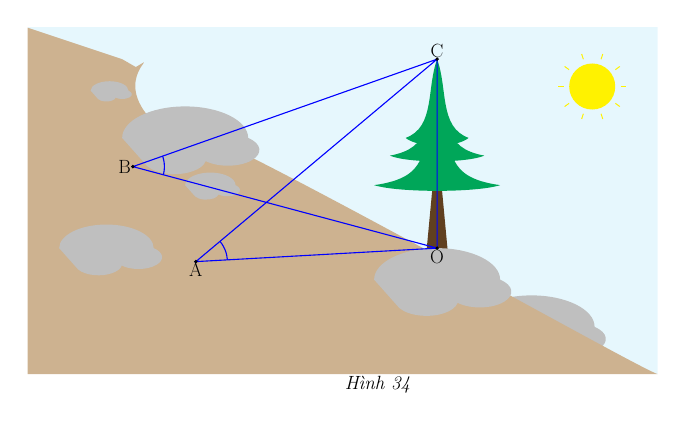
\begin{tikzpicture}[scale=0.4,transform shape,font=\LARGE]
			\draw[draw=none] (0,0)rectangle(20,11);
			\node[below right] at (current bounding box.south) {\textit{Hình 34}};
			\clip (0,0)rectangle(20,11);
			\fill[cyan!10](0,0)rectangle(27,15);
			\tikzset{Icon-mattroi/.pic={
					\def\r{0.35}
					\fill[opacity=1](0,0)circle(\r);
					\draw[line width=2*\r pt](0,0)circle(\r);
					\foreach \g in{1,...,10}{
						\draw[line width=\r pt](\g*36:1.2*\r)++(\g*36:0.1*\r)--++(\g*36:\r*0.25);
					}
			}}
			\tikzset{Doi-Oxyz/.pic={
					\fill[brown!90!teal!60](0,0)--(0,11)--(3,10)--++(-30:0.5)..controls++(-150:-1)and++(135:2)..(4,8)--++(20:0.25)..controls++(60:0.6) and++(160:1)..(20,0)--cycle;
			}}
			\tikzset{da/.pic={
					\fill[gray!50!white](0,0)arc(180:0: 2 and 1)arc(50:-135: 1 and 0.5)arc(-10:-150: 1 and 0.5);
			}}
			\tikzset{cay/.pic={
					\fill[brown!50!black](-0.75,-8)--(0.75,-8)--(0,0)--cycle;
					\fill[green!30!teal][xscale=2,yscale=0.75,shift={(0,-4)}](-2,0)..controls++(-40:1) and++(-140:1)..(2,0)..controls++(160:2)and++(-70:2)..(0,5)..controls++(-110:2)and++(20:2)..(-2,0);
					\fill[green!30!teal][xscale=1.5,yscale=0.75,shift={(0,-1.5)}](-2,0)..controls++(-40:1) and++(-140:1)..(2,0)..controls++(160:2)and++(-70:2)..(0,5)..controls++(-110:2)and++(20:2)..(-2,0);
					\fill[green!30!teal](-2,0)..controls++(-40:1) and++(-140:1)..(2,0)..controls++(160:2)and++(-70:2)..(0,5)..controls++(-110:2)and++(20:2)..(-2,0);
			}}
			\path(14,1.5)pic{da};
			\path(0,0)pic{Doi-Oxyz}(13,7.5)pic[scale=0.5]{cay};
			\foreach \x/\y/\sca in {1/4/0.75,11/3/1,5/6/0.4,3/7.5/1,2/9/0.3}
			\path(\x,\y)pic[scale=\sca]{da};
			\draw[blue](13,10)coordinate(C)--++(220:10)coordinate(A)--(13,4)coordinate(O)--cycle (O)--++(165:10)coordinate(B)--(C);
			\foreach \d in{O,A,B,C}
			\draw[fill=blue](\d)circle(1pt);
			\begin{scope}
				\clip(O)--(A)--(C)--cycle;
				\draw[blue](A)circle(1 cm);
			\end{scope}
			\begin{scope}
				\clip(O)--(B)--(C)--cycle;
				\draw[blue](B)circle(1 cm);
			\end{scope}
			\path(O)node[below]{O}(A)node[below]{A}(B)node[left]{B}(C)node[above]{C}(C)++(-10:5)pic[yellow,scale=2]{Icon-mattroi};
		\end{tikzpicture}
	}
\noindent Tính tổng số đó các góc tạo bởi mỗi dây neo và mặt phẳng sườn núi (làm tròn kết quả đến hàng đơn vị của độ).
\shortans{$92$}
	\loigiai{
	Ta có $\overrightarrow{O A}=(3 ;-4 ; 2), \overrightarrow{O B}=(-5 ;-2 ; 1)$ nên
			$$
			\left[\overrightarrow{OA}, \overrightarrow{O B}\right]=\left(\left|\begin{array}{ll}
				-4 & 2 \\
				-2 & 1
			\end{array}\right| ;\left|\begin{array}{cc}
				2 & 3 \\
				1 & -5
			\end{array}\right| ; \left| \begin{array}{cc}
				3 & -4 \\
				-5 & -2
			\end{array}\right|\right)=(0 ;-13 ;-26).
			$$
			Vì thế, véc-tơ $\overrightarrow{n}=(0 ; 1 ; 2)$ là một véc-tơ pháp tuyến của mặt phẳng $(O A B)$.\\
			Mặt khác, do $\overrightarrow{C A}=(3 ;-4 ;-3)$, $\overrightarrow{B C}=(5 ; 2 ; 4)$ nên ta có
			\[\sin (C A,(O A B))=|\cos (\overrightarrow{CA}, \overrightarrow{n})|=\dfrac{|\overrightarrow{C A} \cdot \overrightarrow{n}|}{|\overrightarrow{C A}| \cdot|\overrightarrow{n}|}=\dfrac{|3 \cdot 0+(-4) \cdot 1+(-3) \cdot 2|}{\sqrt{34} \cdot \sqrt{5}}=\dfrac{10}{\sqrt{170}}.\]
			Suy ra $(C A,(O A B)) \approx 50^{\circ}$. Vậy góc tạo bởi dây neo $C A$ và mặt phẳng sườn núi là khoảng $50^{\circ}$.\\
			Lại có
			$$
			\sin (B C,(O A B))=|\cos (\overrightarrow{B C}, \overrightarrow{n})|=\dfrac{|\overrightarrow{B C} \cdot \overrightarrow{n}|}{|\overrightarrow{B C}| \cdot|\overrightarrow{n}|}=\dfrac{|5 \cdot 0+2 \cdot 1+4 \cdot 2|}{3 \sqrt{5} \cdot \sqrt{5}}=\dfrac{2}{3},
			$$
			suy ra $(B C,(O A B)) \approx 42^{\circ}$. \\
			Vậy góc tạo bởi dây neo $B C$ và mặt phẳng sườn núi là khoảng $42^{\circ}$.\\
			Vậy tổng số đo $2$ góc là $92^\circ$.
	}
\end{ex}

% #4225 | Archive/SP_KhoLatex/SP_Đề Theo Bài-Khối 12/2-B16-De2.tex | mã gốc 2H5V2-7
\begin{ex}%[Nguyễn Tuấn, dự án sáng tác đề 12 theo chủ đề]%[2H5V2-7]
	\immini
	{
		Để chuẩn bị cho chuyến đi dã ngoại, nhóm bạn Đức thiết kế lều cắm trại dạng hình chóp tứ giác đều có đáy là hình vuông cạnh $4$m. Theo bản vẽ thiết kế thì góc giữa hai mặt bên của lều bằng $60^{\circ}$. Bằng phương pháp tọa độ, hãy tính chiều cao của lều này (đơn vị: mét).
		\shortans{$2$}
	}
	{
		\begin{tikzpicture}[>=stealth,line join=round,line cap=round,font=\footnotesize,scale=1]
			\def \cao{3};
			\def \x{3};
			\coordinate (D) at (0,0);
			\coordinate (C) at (1,.8);
			\coordinate (A) at (\x,0);
			\coordinate (B) at ($(A)-(D)+(C)$);
			\coordinate (O) at ($(C)!.5!(A)$);
			\coordinate (S) at ($(O)+(90:\cao)$);
			\coordinate (X) at (intersection of S--O and  D--A);
			\draw (D)--(A)--(B)--(S)--cycle (S)--(A);
			\draw[dashed] (C)--(B) (S)--(C)--(D);
			\draw[dashed,red] (A)--($(A)!1.2!(C)$) (D)--(B) (S)--(X);
			\draw[->,red] (A)--($(O)!1.6!(A)$) node[right]{$x$};
			\draw[->,red] (B)--($(O)!1.4!(B)$) node[above]{$y$};
			\draw[->,red] (S)--($(O)!1.3!(S)$) node[left]{$z$};
			\draw[red] (X)--++(-90:0.7) (D)--($(O)!1.3!(D)$);
			\foreach \diem/\goc in {C/45,D/-90,A/-90,B/-30,S/45,O/-130} \fill[black](\diem) circle (1pt) ($(\diem)+(\goc:3mm)$) node{$\diem$};
		\end{tikzpicture}
	}
	\loigiai{
		Ta có $AC=BD=\sqrt{AD^2+AB^2}=\sqrt{4^2+4^2}=4\sqrt{2}$.\\
		Chọn hệ trục tọa độ $Oxyz$ với gốc tọa độ $O$ là giao điểm của hai đường chéo $AC$ và $BD$ như hình vẽ.\\
		Gọi $z$ là chiều cao của lều.\\
		Ta có $O(0;0;0)$, $A(2\sqrt{2};0;0)$, $B(0;2\sqrt{2};0)$, $C(-2\sqrt{2};0;0)$, $D(0;-2\sqrt{2};0),S(0;0;z)$, với $z>0$.\\
		Ta có $\overrightarrow{AD}=(-2\sqrt{2};-2\sqrt{2};0),\overrightarrow{AB}=(-2\sqrt{2};2\sqrt{2};0),\overrightarrow{AS}=(-2\sqrt{2};0;z)$.\\
		Véc-tơ pháp tuyến của $(SAD)$ là $\overrightarrow{n}_1=\left[\overrightarrow{AD},\overrightarrow{AS}\right]=(-2z\sqrt{2};2z\sqrt{2};-8)$.\\
		Véc-tơ pháp tuyến của $(SAB)$ là $\overrightarrow{n}_2=\left[\overrightarrow{AB},\overrightarrow{AS}\right]=(2z\sqrt{2};2z\sqrt{2};8)$.\\
		Ta có
		\begin{eqnarray*}
			\cos((SAD),(SAB))&=&\dfrac{|\overrightarrow{n}_1\cdot \overrightarrow{n}_2|}{|\overrightarrow{n}_1|\cdot |\overrightarrow{n}_2|}\\
			&=&\dfrac{|-2z\sqrt{2}\cdot 2z\sqrt{2}+2z\sqrt{2}\cdot 2z\sqrt{2}+8\cdot(-8)|}{\sqrt{(-2z\sqrt{2})^2+(2z\sqrt{2})^2+(-8)^2}\cdot \sqrt{(2z\sqrt{2})^2+(2z\sqrt{2})^2+8^2}}\\
			&=&\dfrac{64}{16z^2+64}.
		\end{eqnarray*}
		Vì góc giữa hai mặt bên bằng $60^{\circ}$ nên góc giữa hai mặt phẳng $(SAD)$ và $(SAB)$ bằng $60^{\circ}$.\\
		Do đó
		$$\cos 60^{\circ}=\dfrac{64}{16z^2+64} \Leftrightarrow \dfrac{1}{2}=\dfrac{64}{16z^2+64}\Leftrightarrow 16z^2+64=128\Leftrightarrow \hoac{&z=2\\&z=-2}$$
		Vì $z>0$ nên ta có $S(0;0;2)$.\\
		Vậy chiều cao của lều là $2$ m.
	}
\end{ex}

% #4248 | Archive/SP_KhoLatex/SP_Đề Theo Bài-Khối 12/2-B16-De1.tex | mã gốc 2H5V2-7
\begin{ex}%[2H5V2-7]
	Khi gắn hệ toạ độ $O x y z$ (đơn vị trên mỗi trục tính theo kilômét) vào một sân bay, mặt phẳng $(O x y)$ trùng với mặt sân bay. Một máy bay ở vị trí $A(3 ;-2 ; 3)$ sẽ hạ cánh tới vị trí $B(8 ; 8 ; 0)$. Góc giữa đường bay (một phần của đường thẳng $A B$ ) và sân bay (một phần của mặt phẳng $(O x y)$ ) bằng bao nhiêu độ (làm tròn kết quả đến hàng đơn vị)?
	\begin{center}
	\begin{tikzpicture}[line join = round, line cap = round,>=stealth,font=\footnotesize,scale=.5]
		\path 
		(0,0) coordinate (O)
		(-4,0) coordinate (N)
		($(O)!1!40:(N)$) coordinate (M)
		(0,0.9) coordinate (P)
		($(O)!1.2!(M)$) coordinate (x)
		(-5,0.8) coordinate (A)
		(3,-3) coordinate (B)
		($(A)!2.1cm!(B)$) coordinate (C)
		(intersection of A--B and O--M) coordinate (B1)
		;
		\draw[line width=0.3mm,red] (A)--(C) (B1)--(B);
		\draw[line width=0.3mm,red,dashed] (C)--(B1);
		\draw[->,>=stealth,line width=0.3mm,blue] (0,0)--(x) node[right=0.2cm]{$x$};
		\draw[->,>=stealth,line width=0.3mm,blue] (-5,0)--(-4,0) (0,0) node[above right]{$O$}--(7,0) node[below]{$y$};
		\draw[line width=0.3mm,blue,dashed] (-4,0)--(0,0);
		\draw[->,>=stealth,line width=0.3mm,blue] (0,0)--(0,3) node[left]{$z$};
		\foreach \x/\gm in {A/90,B/90} \fill (\x) circle (1pt) ($(\x)+(\gm:5mm)$)node[blue]{$\x$};	
	\end{tikzpicture}
	\end{center}
	
	\shortans{$15$}
	\loigiai{
		Đường thẳng $A B$ có véc-tơ chỉ phương là $\overrightarrow{u}=(5 ; 10 ;-3)$, mặt phẳng $(O x y)$ có véc-tơ pháp tuyến là $\overrightarrow{k}=(0 ; 0 ; 1)$. \\
		Gọi $\alpha$ là góc giữa đường bay (một phần của đường thẳng $A B$ ) và sân bay (một phần của mặt phẳng $(O x y)$). Khi đó
		$\sin \alpha=\dfrac{|\overrightarrow{k} \cdot \overrightarrow{u}|}{|\overrightarrow{k}| \cdot|\overrightarrow{u}|}=\dfrac{3}{\sqrt{134}}$.\\
		Suy ra $\alpha \approx 15^{\circ}$.
		
	}
\end{ex}

% #4250 | Archive/SP_KhoLatex/SP_Đề Theo Bài-Khối 12/2-B16-De1.tex | mã gốc 2H5C2-7
\begin{ex}%[2H5C2-7]
	Cho biết kim tự tháp Memphis tại bang Tennessee (Mỹ) có dạng hình chóp tứ giác đều $S.ABCD$ với chiều cao $98$ m và cạnh đáy $180$ m. Số đo góc giữa hai mặt bên bằng bao nhiêu độ (làm tròn kết quả đến hàng đơn vị)?
	\shortans{$63$}
	\loigiai{
	\immini{
	Gọi $O=AC \cap BD$. Vì $S.ABCD$ là hình chóp đều nên $S O \perp(A B C D)$.\\
	Ta có $AC=BD=AB \sqrt{2}=180 \sqrt{2}$.\\
	Chọn hệ trục $Oxyz$ như hình vẽ với $O(0;0;0)$, $C(90 \sqrt{2} ; 0 ; 0)$, $D(0 ; 90 \sqrt{2} ; 0)$, $B(0;-900\sqrt{2};0)$ và $S(0 ; 0 ; 98)$.
}
{
	\begin{tikzpicture}[scale=0.55, font=\footnotesize, line join=round, line cap=round, >=stealth]
		\def\bc{5} % cạnh BC
		\def\ba{3.5} % cạnh BA
		\def\h{5} % đường cao
		\def\gocB{40} % góc B của đáy
		\coordinate (B) at (0,0);
		\coordinate (A) at (\gocB:\ba);
		\coordinate (C) at (\bc,0);
		\coordinate (D) at ($(C)-(B)+(A)$);
		\coordinate (O) at ($(A)!.5!(C)$);
		\coordinate (S) at ($(O)+(90:\h)$);
		\coordinate (z) at ($(O)+(90:\h+1)$);
		\coordinate (y) at ($(O)!1.25!(D)$);
		\coordinate (x) at ($(O)!1.5!(C)$);
		\draw (B)--(C)--(D)--(S)--cycle (S)--(C);
		\draw[dashed] (C)--(A)--(D)--(B) (O)--(S)--(A)--(B);
		\draw [->] (S)--(z);
		\draw [->] (D)--(y);
		\draw [->] (C)--(x);
		\foreach \p/\i in {S/180, A/180,B/-60,D/40,C/-120,O/170}
		\fill (\p) circle (1.5pt) node[shift={(\i:3mm)}]{$\p$};
		\foreach \p/\i in {z/180,y/-90,x/40}
		\fill (\p)  node[shift={(\i:3mm)}]{$\p$};
\end{tikzpicture}}
\noindent
	Phương trình mặt phẳng $(SBC)$ dưới dạng đoạn chắn là
	$$ \dfrac{x}{90\sqrt{2}}+\dfrac{y}{-90 \sqrt{2}}+\dfrac{z}{98}=1\qquad \text{hay } 49x-49y+45\sqrt{2} z-4410 \sqrt{2}=0.$$
Phương trình mặt phẳng $(SCD)$ dưới dạng đoạn chắn là\\ $ \dfrac{x}{90 \sqrt{2}}+\dfrac{y}{90 \sqrt{2}}+\dfrac{z}{98}=1$ hay $49x+49y+45\sqrt{2} z-a \sqrt{2}=0$.\\
Khi đó hai mặt phẳng $(SBC)$ và $(SCD)$ có véc-tơ pháp tuyến lần lượt là  $\overrightarrow{n}_1=(49 ; -49 ; 45\sqrt{2})$, $\overrightarrow{n}_2=(49 ; 49 ; 45\sqrt{2})$.\\
Suy ra $$\cos ((S BC),(SCD))=\dfrac{|\overrightarrow{n}_1 \cdot \overrightarrow{n}_2|}{|\overrightarrow{n}_1| \cdot|\overrightarrow{n}_2|}=\dfrac{\left|49\cdot 49-49\cdot 49+45\sqrt{2}\cdot 45\sqrt{2} \right| }{\sqrt{49^2+(-49)^2+(45\sqrt{2})^2}\cdot \sqrt{49^2+49^2+(45\sqrt{2})^2}}=\dfrac{\sqrt{2025}}{4426}.$$ 
Do đó $((SBC),(SCD))\approx 63^{\circ}$.
}
\end{ex}

% #4276 | Archive/SP_KhoLatex/SP_Bộ đề OTK12/SP_Data/2-OTC5-De1.tex | mã gốc 2H5V2-7
\begin{ex}%[2H5V2-7]
	Hình bên dưới minh họa đường bay của một chiếc trực thăng $H$ cất cánh từ một sân bay. Xét hệ trục tọa độ $Oxyz$ có gốc tọa độ $O$ là chân tháp điều khiển của sân bay; trục $Ox$ là hướng đông, trục $Oy$ là hướng Bắc và trục $Oz$ là trục thẳng đứng, đơn vị trên mỗi trục là kilômét.\\
	Trực thăng cất cánh từ điểm $G$. véc-tơ $\vec{r}$ chỉ vị trí của trực thăng tại thời điểm $t$ phút sau khi cất cánh $(t\ge 0)$ có tọa độ là $\vec{r}=(1+t; 0,5+2t; 2t)$.
	\begin{center}
		\begin{tikzpicture}
			\coordinate (O) at (0,0);
			\coordinate (z) at (0,3);
			\coordinate (x) at (2.5,-1.5);
			\coordinate (y) at (5,2);
			\coordinate (Oxy) at ($(y)+(2.5,-1.5)$);
			
			\path[fill=cyan!15] (O)--(x)--(Oxy)--(y)--cycle;
			\coordinate (G) at (1.5,0);
			\coordinate (F) at (4,0);
			\coordinate (F') at (5,0);
			\coordinate (H) at ($(F)+(0,3.5)$);
			\draw[->] (G)--(H);
			\draw[dashed] (G)--(F') (H)--(F);
			\draw ($(F)+(-0.2,0)$)|-($(F)+(0,0.2)$);
			\begin{scope}
				\clip (F)--(G)--(H);
				\draw (G) circle(0.4);
			\end{scope}
			\draw[->] (O)--(x);
			\draw[->] (O)--(y);
			\draw[->] (O)--(z);
			\foreach \x in{G,H,F}{
				\fill (\x) circle(1pt);
			}
			\path 
			node at (O) [below]{$O$}
			node at (z) [left]{$z$}
			node at (x) [below]{$x$ (Đ)}
			node at (y) [above right]{$y$ (B)}
			node at (G) [below]{$G$}
			node at (F) [below]{$F$}
			node at (H) [right]{$H$}
			node at ($(G)+(30:0.6)$) {$\theta$}
			;
		\end{tikzpicture}
	\end{center}
	Mỗi mệnh đề sau là đúng hay sai?
	\choiceTF
		{Góc $\theta$ mà đường bay tạo với phương ngang làm tròn đến phút là $45^\circ$}
		{\True Phương trình đường thẳng $GF$, trong đó $F$ là hình chiếu của điểm $H$ lên mặt phẳng $(Oxy)$ là $\heva{&x=1+t\\&y=0,5+2t\\&z=0}$, $t\in \mathbb{R}$}
		{\True Trực thăng bay vào mây ở độ cao $2$ km. Tọa độ điểm mà máy bay trực thăng bắt đầu đi vào đám mây là $(2;2{,}5;2)$}
		{Giả sử một đỉnh núi nằm ở điểm $M(5;4,5;3)$. Khi $HM$ vuông góc với đường bay $GH$ thì khoảng cách từ máy bay trực thăng đến đỉnh núi tại thời điểm đó là $3$km}
	\loigiai{
		\begin{itemchoice}
			\itemch Ta có phương trình tham số của đường thẳng $GH$ là $\heva{&x=1+t \\&y=0,5+2t\\ & z=2t}$, $t\in \mathbb{R}$.\\
			\allowdisplaybreaks
			\begin{eqnarray*}
			\sin \left(d; (Oxy)\right) &=& \left|\cos\left(\vec{u}_{d}; \vec{n}_{Oxy}\right)\right|\\
			&=& \dfrac{\left|\vec{u}_{d}\cdot \vec{n}_{Oxy}\right|}{\left|\vec{u}_{d}\right| \cdot \left| \vec{n}_{Oxy}\right|}\\
			&=& \dfrac{\left|1\cdot 0 + 2\cdot 0 + 2\cdot 1\right|}{\sqrt{1^2+2^2+2^2} \cdot \sqrt{0^2+0^2+1^2}}=\dfrac{2}{3}.	
			\end{eqnarray*}
			Suy ra $\left(d;(Oxy)\right)\approx 41^{\circ} 49'$. \\
			Vậy góc $\theta$ mà đường bay tạo với phương ngang xấp xỉ $41^{\circ} 49'$.
			\itemch Ta có điểm $M\left(2;2,5;4\right)$ nằm trên đường thẳng $GH$.\\ 
			Hình chiếu của $M$ lên mặt phẳng $(Oxy)$ là $N(2;2,5;0)$ và điểm $N$ nằm trên đường thẳng $GF$.\\
			Vậy $GF$  đi qua $G(1;0,5;0)$ và nhận véc-tơ $\vec{GN}=(1;2;0)$ làm véc-tơ chỉ phương, do đó có phương trình là $\heva{&x=1+t\\&y=0,5+2t\\&z=0}$, $t\in \mathbb{R}$.
			\itemch Trực thăng bay vào mây ở độ cao $2$ km, khi đó ta có 
			$2t=2 \Leftrightarrow t=1$. Tọa độ điểm mà máy bay bắt đầu đi vào mây là $(2;2{,}5;2)$.
			\itemch Gọi $H(1+t; 0,5+2t;2t)$ là vị trí cần tìm. Ta có $\vec{HM}=(4-t; 4-2t; 3-2t)$. \\
			Ta có $HM \perp GH$ suy ra $$\vec{HM}\cdot \vec{u}_{GH} = 0 \Leftrightarrow (4-t)\cdot 1 + (4-2t)\cdot 2 + (3-2t) \cdot 2 =0 \Leftrightarrow t=2.$$
			Vậy $H(3;4,5;4)$.\\
			Khoảng cách từ trực thăng đến đỉnh núi là $$MH = \sqrt{(3-5)^2+(4,5-4,5)^2+(4-3)^2} =\sqrt{5} \approx 2,236 \text{ km.}$$ 
			\itemch  
			\begin{center}
				\begin{tikzpicture}
					\coordinate (O) at (0,0);
					\coordinate (z) at (0,3);
					\coordinate (x) at (2.5,-1.5);
					\coordinate (y) at (5,2);
					\coordinate (Oxy) at ($(y)+(2.5,-1.5)$);
					
					\path[fill=cyan!15] (O)--(x)--(Oxy)--(y)--cycle;
					\coordinate (G) at (1.5,0);
					\coordinate (F) at (4,0);
					\coordinate (F') at (5,0);
					\coordinate (H) at ($(F)+(0,3.5)$);
					\draw[->] (G)--(H);
					\draw[dashed] (G)--(F') (H)--(F);
					
					\draw ($(F)+(-0.2,0)$)|-($(F)+(0,0.2)$);
					\begin{scope}
						\clip (F)--(G)--(H);
						\draw (G) circle(0.4);
					\end{scope}
					\draw[->] (O)--(x);
					\draw[->] (O)--(y);
					\draw[->] (O)--(z);
					\foreach \x in{G,H,F}{
						\fill (\x) circle(1pt);
					}
					\path 
					node at (O) [below]{$O$}
					node at (z) [left]{$z$}
					node at (x) [below]{$x$ (Đ)}
					node at (y) [above right]{$y$ (B)}
					node at (G) [below]{$G$}
					node at (F) [below]{$F$}
					node at (H) [right]{$H$}
					node at ($(G)+(30:0.6)$) {$\theta$}
					;
				\end{tikzpicture}
			\end{center}
		\end{itemchoice}
	}
\end{ex}

% #4281 | Archive/SP_KhoLatex/SP_Bộ đề OTK12/SP_Data/2-OTC5-De1.tex | mã gốc 2H5C3-4
\begin{ex}%[2H5C3-4]
	Trong không gian với hệ tọa độ $Oxyz$, đài kiểm soát không lưu sân bay có tọa độ $O(0;0;0)$, mỗi đơn vị trên trục ứng với $1$ km. Máy bay bay trong phạm vi cách đài kiểm soát $417$ km sẽ hiển thị trên màn hình ra đa. Một máy bay đang ở vị trí $A\left(-688;-185;8\right)$, chuyển động theo đường thẳng $d$ có véc-tơ chỉ phương là $\vec{u}=(91;75;0)$ và hướng về đài kiểm soát không lưu.
	\begin{center}
		\begin{tikzpicture}
			\def\r{3}
			\def \x{3}  %bán kính trục lớn elip
			\def \y{1.2} 
			\coordinate (o1) at (-\r,0);
			\coordinate (o2) at (\r,0);
			\coordinate (O) at (0,0);
			
			% ve mp
			\coordinate (P) at (-5,2);
			\coordinate (Q) at ($(P)+(240:6)$);
			\coordinate (R) at ($(Q)+(12,0)$);
			\coordinate (S) at ($(R)+(60:6)$);
			\fill[cyan!20] (P)--(Q)--(R)--(S)--cycle;
			
			
			\draw (O) circle(\r); 
			\path[fill=orange!20] (O) circle(\r); 
			\fill[orange!80] (o2) arc (0:-180:\x cm and \y cm) arc (180:360:\x cm and \x cm);
			\draw[dashed] (o2) arc (0:180:\x cm and \y cm);
			\draw (o2) arc (0:-180:\x cm and \y cm);
			
			% truc oz
			\coordinate (Oz) at (0,4.5);
			\coordinate (Oz') at (0,2.5);
			\coordinate (Oz'') at (0,-3.5);
			\draw[dashed] (Oz'')--(Oz');
			\draw[->] (Oz')--(Oz);
			% tru  ox
			\def\t{240}
			\coordinate (Ox) at ({\x*cos(\t)},{\y*sin(\t)});
			\coordinate (Ox') at ($(O)!2!(Ox)$);
			\coordinate (Ox'') at ($(Ox)!2.2!(O)$);
			\draw[dashed] (O)--(Ox);
			\draw[->] (Ox)--(Ox');
			\draw[dashed] (O)--(Ox'');
			% truc oy
			\coordinate (O4) at (\r,0);
			\coordinate (O5) at (1.5*\r,0);
			\coordinate (O2) at (-\r,0);
			\coordinate (O1) at (-1.5*\r,0);
			\draw (O1)--(O2);
			\draw[dashed] (O2)--(O4);
			\draw[->] (O4)--(O5);
			% duong d
			\coordinate (A) at (-4.52,1.7);
			\coordinate (A3) at (4.5,0.3);
			\coordinate (A1) at ($(A)!0.25!(A3)$);
			\coordinate (A2) at ($(A)!0.82!(A3)$);
			\draw (A)--(A1);
			\draw[dashed] (A1)--(A2);
			\draw (A2)--(A3);
			\foreach \x in {O}{
				\fill (\x) circle(1pt);
			}
			\path 
			node at (O) [above left]{$O$}
			node at (A) [above] {$A$}
			node at (A1) [above]{B}
			node at (A2) [above right]{$C$}
			node at (A3) [above]{$d$}
			node at (Oz) [left]{$z$}
			node at (O5) [below]{$y$}
			node at (Ox')[below]{$x$}
			;
		\end{tikzpicture}
	\end{center}
	Tọa độ của vị trí sớm nhất mà máy bay xuất hiện trên màn hình ra đa là $M(a;b;c)$. Khi đó $a+b+c$ bằng
	\shortans{$-458$}
	\loigiai{
		Đường thẳng $d$ đi qua $A(-688;-185;8)$, có véc-tơ chỉ phương là $\vec{u}=(91;75;0)$ nên có phương trình tham số là $\heva{& x=-688 +91t \\ &y=-185+75t\\ &z=8}, t\in \mathbb{R}$.\\
			Mặt cầu $(S)$ tâm $O(0;0;0)$ bán kính $R=417$ có phương trình $x^2+y^2+z^2=173\,889$.\\
			Tọa độ giao điểm của đường thẳng $d$ và mặt cầu $(S)$ là nghiệm của hệ 
			\begin{eqnarray*}
				\heva{&x=-688 +91t \\ &y=-185+75t\\ &z=8 \\& x^2+y^2+z^2=173\,889} 
				&\Leftrightarrow & 
				\heva{&x=-688 +91t \\ &y=-185+75t\\ &z=8 \\& (-688+91t)^2+(-185+75t)^2+8^2=173\,889} \\
				& \Leftrightarrow & 	\heva{&x=-688 +91t \\ &y=-185+75t\\ &z=8 \\& \hoac{&t=8 \\&t=3.}}  
			\end{eqnarray*}
			Với $t=8 \Rightarrow $ tọa độ giao điểm thứ nhất là $M_1 (40;415;8)$.\\
			Với $t=3 \Rightarrow $ tọa độ giao điểm thứ hai là $M_2 (-506; 40;8)$.\\
			Ta có $AM_1 = \sqrt{889984}$ và $AM_2 = \sqrt{76869}$, suy ra $AM_2 < AM_1$. Vậy tọa độ của vị trí sớm nhất mà máy bay xuất hiện trên màn hình ra đa là $M_2=(-506;40;8)$.\\
			Điểm $M_2$ chính là điểm $B$ trên hình vẽ.\\
			Suy ra $a=-506$, $b=40$ và $c=8$. Vậy $a+b+c=-458$.
	}
\end{ex}

% #4370 | Archive/SP_KhoLatex/SP_Bộ đề OTK12/SP_Data/2-OTGK2-De1.tex | mã gốc 2H5C2-3
\begin{ex}%[2H5C2-3]
	Trong không gian với hệ tọa độ $Oxyz$, một cabin cáp treo xuất phát từ điểm $A(10;3;0)$ và chuyển động đều theo đường cáp có véc-tơ chỉ phương là $\vv{u}=(2;-2;1)$ với tốc độ là $4{,}5$ m/s (đơn vị trên mỗi trục tọa độ là mét). Cabin dừng ở điểm $B$ có hoành độ $x_B=550$. Tìm độ dài quãng đường $AB$ (làm tròn kết quả đến hàng đơn vị của mét).
	\begin{center}
		\begin{tikzpicture}[line join=round,line cap=round,>=stealth,scale=0.75,font=\footnotesize]
			\tikzset{every node/.style={outer sep=-0.5mm}}
			\foreach \x/\y/\n in {0/0/O,5/0/y,0/4/z,-4/-4/x,-5/2.5/B} \coordinate (\n) at (\x,\y);
			\coordinate (C) at ($(O)!0.1!(y)$);
			\coordinate (D) at ($(O)!0.15!(x)$);
			\coordinate (A) at ($(C)+(D)-(O)$);
			\coordinate (E) at ($(O)!0.8!(x)$);
			\coordinate (M) at ($(A)!0.65!(B)$);
			\coordinate (v) at ($(A)!0.15!(B)$);
			\coordinate (u) at ($(O)+(v)-(A)$);
			\draw[->] (O)--(x) node[right] {\normalsize$x$};
			\draw[->] (O)--(y) node[below left] {\normalsize$y$};
			\draw[->] (O)--(z) node[below left] {\normalsize$z$};
			\draw[dashed,thin](C)--(A)--(D) (B)node[above]{$B$}--(E)node[below right]{$550$};
			\draw (E) node[left]{$x_B$};
			\draw (O) node[above right]{$O$};
			\draw (C) node[below]{$3$};
			\draw (D) node[left]{$10$};
			\fill (A) circle (1.5pt) node[below right] {$A(10;3;0)$};
			\draw[very thick] (A)--(B);
			\draw[->,very thick,red] (O)--(u)node[above]{$\vv{u}$};
			\fill[red] (M) circle (2pt) node[above right] {$M$};
			\draw (M) .. controls ($(M)+(-0.2,-0.1)$) .. ($(M)+(0,-0.2)$) node[below,yshift=1mm]{{\large \faCube}};
			%			\draw ($(O)+(0,-4)$) node[below]{\textit{Hình 35}};
		\end{tikzpicture}
	\end{center}
	\shortans{$810$}
	\loigiai{
		\begin{itemize}
			\item Phương trình chính tắc của đường cáp là $\dfrac{x-10}{2}=\dfrac{y-3}{-2}=\dfrac{z}{1}$.
			\item Do tốc độ chuyển động của cabin là $4{,}5$ m/s nên độ dài $AM=4{,}5t$ (m). \\
			Vì vậy $\left|\vv{AM}\right|=4{,}5t$ ($t\ge0$).\\
			Do hai véc-tơ $\vv{AM}$ và $\vv{u}$ là cùng hướng nên $\vv{AM}=k\vv{u}$ với $k\in\mathbb{R}^+$.\\
			Suy ra $\left|\vv{AM}\right|=k\left|\vv{u}\right|=k\cdot\sqrt{2^2+(-2)^2+1^2}=3k$. Do đó $3k=4{,}5t\Leftrightarrow k=\dfrac{3t}{2}$. \\
			Vì thế, ta có $\vv{AM}=\dfrac{3t}{2}\vv{u}=\left(3t;-3t;\dfrac{3t}{2}\right)$.\\
			Gọi tọa độ của điểm $M$ là $(x_M;y_M;z_M)$.\\
			Do $\vv{AM}=(x_M-x_A;y_M-y_A;z_M-z_A)=\left(3t;-3t;\dfrac{3t}{2}\right)$ nên $$\heva{&x_M=3t+x_A\\&y_M=-3t+y_A\\&z_M=\dfrac{3t}{2}+z_A}\Leftrightarrow\heva{&x_M=3t+10\\&y_M=-3t+3\\&z_M=\dfrac{3t}{2}.}$$
			Vậy điểm $M$ có tọa độ là $\left(3t+10;-3t+3;\dfrac{3t}{2}\right)$.
			\item Do $x_B=550$ nên $3t+10=550$, tức là $t=180$ (s). Do đó, ta có điểm $B(550;-537;270)$.\\
			Vậy $AB=\sqrt{(550-10)^2+(-537-3)^2+(270-0)^2}=\sqrt{656100}=810$ (m).
		\end{itemize}
	}
\end{ex}

% #4375 | Archive/SP-4Phan-Dot3/Data/CD_2-OTHK2-De05.tex | mã gốc 2H5V3-4
\begin{ex}%[Dự án Đề thi 4 phần-Đợt 3]%[Đắc Vũ]%[2H5V3-4]
	Trong không gian $Oxyz$, đài kiểm soát không lưu sân bay có tọa độ $O(0; 0; 0)$, mỗi đơn vị trên trục ứng với $1$ km. Máy bay bay trong phạm vi cách đài kiểm soát $417$ km sẽ hiển thị trên màn hình ra đa. Một máy bay đang ở vị trí $A(-688; -185; 8)$, chuyển động theo đường thẳng $d$ có véc-tơ chỉ phương là $\vec{u} = (91; 75; 0)$ và hướng về đài kiểm soát không lưu. Biết rằng  tọa độ của vị trí sớm nhất mà máy bay xuất hiện trên màn hình radar là $B(a;b;c)$. Tính $S=a+5b+2c$.
	\shortans{$-199$}
	\loigiai{
		\begin{center}
			\begin{tikzpicture}[line join = round, line cap=round,>=stealth,font=\footnotesize,scale=1]
				\def \daiE{2}
				\path 	
				(0,0)coordinate (X1)
				--(7,0)coordinate (X2)
				--(9,5)coordinate (X3)
				--($(X1)+(X3)-(X2)$)coordinate (X4)
				--cycle
				($(X2)!1/2!(X4)$) coordinate (tamE)
				($(tamE)-(\daiE,0)$) coordinate (Etrai)
				($(tamE)+(\daiE,0)$) coordinate (Ephai)
				($(tamE)+(160:2)$) coordinate (B)
				($(tamE)+(10:2)$) coordinate (C)
				;
				\draw[fill=cyan,opacity=0.2] (X1)--(X2)-- (X3)--(X4)--cycle;
				\draw[dashed] (tamE) ellipse (\daiE cm and 1cm)(B)--(C);
				\draw (Ephai) arc(0:-180:\daiE cm and 1cm); 		
				\draw[->,dashed] ($(Etrai)!-0.2!(Ephai)$)--($(Etrai)!1.2!(Ephai)$) node[below]{$y$};
				\draw[->,dashed] ($(tamE)+(1.5,1.5)$)--($(tamE)+(-1.5,-1.5)$) node[below]{$x$};
				\draw[->,dashed] ($(tamE)+(0,-2)$)--($(tamE)+(0,3)$) node[above]{$z$};
				\draw[fill=red,opacity=0.4] (tamE) circle(2cm);
				\draw[fill=brown,opacity=0.2] (Ephai) arc(0:-180:\daiE cm and 1cm)--(Etrai) arc(180:360:2cm and 2cm);
				\draw 
				(tamE) circle(1pt) node[below right]{$O$}
				(B) circle(1pt) node[above right]{$B$}
				(C) circle(1pt) node[above right]{$C$}
				(B)--($(B)!-0.2!(C)$)node[above]{$A$}
				(C)--($(B)!1.2!(C)$)node[above]{$d$}
				;
			\end{tikzpicture}
		\end{center}
		Phương trình mặt cầu mô tả ranh giới bên ngoài vùng phát sóng của radar trong không gian là $(S) \colon x^2+y^2+z^2=417^2$. \\
		Phương trình tham số của đường thẳng $d$ đi qua $A(-688 ;-185 ; 8)$ và nhận $\vec{u}=(91 ; 75 ; 0)$ làm véc-tơ chỉ phương là $\heva{&x=-688+91t\\& y=-185+75t\\&z=8.}$\\
		Gọi $B$ là vị trí sớm nhất mà máy bay xuất hiện trên màn hình radar. \\
		Vì $B \in d \Rightarrow B(-688+91 t ;-185+75 t ; 8)$.
		Vì $B$ là vị trí sớm nhất mà máy bay xuất hiện trên màn hình radar nên
		\begin{eqnarray*}
			&&(-688+91 t)^2+(-185+75 t)^2+8^2=417^2\\
			&\Rightarrow &13906 t^2-152966 t+333744=0\\
			&\Rightarrow &\hoac{&t=3 \\
				&t=8.}
		\end{eqnarray*}
		Với $t=3 \Rightarrow B(-415 ; 40 ; 8) \Rightarrow A B \approx 353{,}77$ km. \\
		Với $t=8 \Rightarrow B(-88 ; 415 ; 8) \Rightarrow A B \approx 848{,}53$ km.\\
		Do $353{,}77<848{,}53$ vị trí máy bay xuất hiện sớm nhất là $B(-415 ; 40 ; 8)$.
		
	}
\end{ex}

% #4406 | Archive/SP-4Phan-Dot3/Data/KNTT_2-OTGK2_De02.tex | mã gốc 2H5V1-7
\begin{ex}%[2H5V1-7]
	Một sân vận động được xây dựng theo mô hình là hình chóp cụt $OAGD.BCFE$ có hai đáy song song với nhau. Mặt sân $OAGD$ là hình chữ nhật và được gắn hệ trục $Oxyz$ như hình vẽ dưới (đơn vị trên mỗi trục tọa độ là mét). Mặt sân $OAGD$ có chiều dài $OA=100$ m, chiều rộng $OD=60$ m và tọa độ điểm $B(10;10;8)$. Khoảng cách từ điểm $G$ đến mặt phẳng $(OBED)$ bằng bao nhiêu mét? (kết quả viết dưới dạng số thập phân và làm tròn đến hàng phần chục).
	\begin{center}
		\begin{tikzpicture}[line join=round, line cap=round,thick,>=stealth,scale=0.5]
			\def \k{0.6}
			\coordinate (O) at (0,0);
			\coordinate (A) at (10:10);
			\coordinate (D) at (150:6);
			\coordinate (G) at ($(A)+(D)-(O)$);
			\coordinate (S') at ($(A)!0.5!(D)$);
			\coordinate (S) at ($(S')+(0,7)$);
			\coordinate (B) at ($(S)!\k!(O)$);
			\coordinate (E) at ($(S)!\k!(D)$);
			\coordinate (F) at ($(S)!\k!(G)$);
			\coordinate (C) at ($(S)!\k!(A)$);
			\coordinate (z) at (90:7);
			\coordinate (x) at ($(O)!1.25!(A)$);
			\coordinate (y) at ($(O)!1.25!(D)$);
			\foreach \i/\j in {E/D,D/O,O/A,O/B,A/C,E/B,B/C,C/F,F/E}{\draw (\i)--(\j);}
			\foreach \i/\j in {D/G,F/G,G/A}{\draw[dashed,thin](\i)--(\j);}
			\draw [->] (O)--(z) node[left]{$z$};
			\draw [->] (A)--(x) node[below]{$x$};
			\draw [->] (D)--(y) node[below]{$y$};
			\foreach \i/\g in {A/-90,G/150,O/-90,D/250,B/-40,E/120,F/70,C/30}{\draw[fill=black](\i) circle (1.5pt) ($(\i)+(\g:5mm)$) node[scale=0.8]{$\i$};}
		\end{tikzpicture}
	\end{center}
	
	\shortans{62{,}5}
	\loigiai{
		\begin{center}
			\begin{tikzpicture}[line join=round, line cap=round,thick,>=stealth,scale=0.5]
				\def \k{0.6}
				\coordinate (O) at (0,0);
				\coordinate (A) at (10:10);
				\coordinate (D) at (150:6);
				\coordinate (G) at ($(A)+(D)-(O)$);
				\coordinate (S') at ($(A)!0.5!(D)$);
				\coordinate (S) at ($(S')+(0,7)$);
				\coordinate (B) at ($(S)!\k!(O)$);
				\coordinate (E) at ($(S)!\k!(D)$);
				\coordinate (F) at ($(S)!\k!(G)$);
				\coordinate (C) at ($(S)!\k!(A)$);
				\coordinate (z) at (90:7);
				\coordinate (x) at ($(O)!1.25!(A)$);
				\coordinate (y) at ($(O)!1.25!(D)$);
				\foreach \i/\j in {E/D,D/O,O/A,O/B,A/C,E/B,B/C,C/F,F/E}{\draw (\i)--(\j);}
				\foreach \i/\j in {D/G,F/G,G/A}{\draw[dashed,thin](\i)--(\j);}
				\draw [->] (O)--(z) node[left]{$z$};
				\draw [->] (A)--(x) node[below]{$x$};
				\draw [->] (D)--(y) node[below]{$y$};
				\foreach \i/\g in {A/-90,G/150,O/-90,D/250,B/-40,E/120,F/70,C/30}{\draw[fill=black](\i) circle (1.5pt) ($(\i)+(\g:5mm)$) node[scale=0.8]{$\i$};}
			\end{tikzpicture}
		\end{center}
		Gắn hình chóp cụt $OAGD.BCFE$ vào hệ trục $Oxyz$, ta có
		$O(0;0;0)$, $A(100;0;0)$, $G(100;60;0)$, $D(0;60;0)$, $B(10;10;8)$.\\
		Lúc đó
		$\overrightarrow{OD}=(0;60;0)$, $\overrightarrow{OB}=(10;10;8)$.\\
		Vectơ pháp tuyến của mặt phẳng $(OBED)$ là $$\overrightarrow{n}=\left[\overrightarrow{OD},\overrightarrow{OB}\right]=(480;0;-600)=120(4;0;-5).$$
		Mặt phẳng $(OBED)$ đi qua điểm $O(0;0;0)$ và có vectơ pháp tuyến $\overrightarrow{n}=(4;0;-5)$ có phương trình là $4x-5z=0$.\\
		Khoảng cách từ điểm $G$ đến mặt phẳng $(OBED)$ là
		$$\mathrm{d}\Big(G,(OBED)\Big)=\dfrac{|4\cdot 100-5\cdot 0 |}{\sqrt{16+25}}=\dfrac{400\sqrt{41}}{41}\approx 62{,}5\,\mathrm{m}.$$		
	}
\end{ex}

% #4416 | Archive/SP-4Phan-Dot3/Data/CD_2-OTHK2-De01.tex | mã gốc 2H5V3-4
\begin{ex}%[Dự án đè thi 4 phần đợt 3]%[Trần Xuân Hòa]%[2H5V3-4]
	Trong không gian $Oxyz$ (đơn vị các trục tọa độ là mét), một quả bóng hình cầu có phương trình bề mặt $(S) \colon (x-3)^2+(y-4)^2+(z-2)^2=\dfrac{1}{625}$ bị rơi xuống bể bơi. Do chất liệu đặc biệt nên phân nửa quả bóng nằm bên dưới mặt nước, phân nửa còn lại ở trên. Tính độ cao mực nước biết đáy bể thuộc mặt phẳng $(Oxy)$.
	\shortans{$2$}
	\loigiai{
		Độ cao mực nước bằng khoảng cách từ tâm $I(3;4;2)$ của mặt cầu đến mặt phẳng $(Oxy)$.\\
		Ta có $\mathrm{d}(I,(Oxy))=2$.\\
		Vậy độ cao mực nước là $2$ mét.
	}
\end{ex}

% #4433 | Archive/SP-4Phan-Dot3/Data/CTST_0-OTGK2_De03.tex | mã gốc 2H5V2-8
\begin{ex}%[2H5V2-8]%[Dự án đề 4 phần]$[Tex hóa: Lê Thị Thúy Hằng]
Trường $A$ có $100$ cán bộ công nhân viên và muốn tổ chức cho toàn trường đi nghỉ mát tại đảo Cát Bà thuộc huyện Cát Hải, thành phố Hải Phòng. Một công ty du lịch chào giá vé với trường như sau:
\begin{itemize}
	\item $40$ khách hàng đầu tiên có giá vé là $3$ triệu đồng/người.
	\item Nếu có nhiều hơn $40$ người đăng kí thì cứ thêm $1$ người giá vé sẽ giảm $15\,000$ đồng/người cho toàn bộ hành khách.
\end{itemize}
Tìm số cán bộ công nhân viên tối thiểu của trường A tham gia đi nghỉ mát để lợi nhuận tối thiểu của công ty du lịch là $45$ triệu đồng. Biết chi phí thực tế công ty dành cho mỗi khách hàng là $1{,}95$ triệu đồng.
\shortans[]{$50$}
\loigiai{
	Gọi $x$ $(x\in \mathbb{N})$ là số lượng cán bộ công nhân viên của trường đăng kí từ thứ $41$ trở lên.\\
	Vì cứ nhiều hơn $40$ người đăng kí thì cứ thêm $1$ người giá vé sẽ giảm $15\,000$ đồng/người cho toàn bộ hành khách nên thêm $x$ người giá vé còn $3\,000-15x$ (nghìn đồng/người).\\
	Doanh thu của công ty du lịch là $(3\,000-15x)(40+x)$ (nghìn đồng).\\
	Chi phí thực tế cho chuyến đi là $1\,950(40+x)$ (nghìn đồng).\\
	Lợi nhuận của công ty du lịch đạt được là
	\allowdisplaybreaks
	\begin{eqnarray*}
		T&=&(3\,000-15x)(40+x)-1\,950(40+x)\\
		&=&-15x^2-600x+3\,000x+120\,000-1\,950x-78\,000\\
		&=&-15x^2+450x+42\,000 \text{ (nghìn đồng).}
	\end{eqnarray*}
	Để lợi nhuận công ty tối thiểu là $45$ triệu đồng thì
	\allowdisplaybreaks
	\begin{eqnarray*}
		&&T\ge 45\,000\\
		&\Leftrightarrow&-15x^2+450x+42\,000\ge 45\,000\\
		&\Leftrightarrow&-15x^2+450x-3\,000\ge 0\\
		&\Leftrightarrow&10\le x\le 20.
	\end{eqnarray*}
	Vậy số cán bộ công nhân viên trường đăng ký tối thiểu là $50$ người thì công ty du lịch đạt lợi nhuận tối thiểu $45$ triệu đồng.	
}
\end{ex}

% #4444 | Archive/SP-4Phan-Dot3/Data/KNTT_2-OTHK2_De01.tex | mã gốc 2H5V3-43
\begin{ex}%[Dự án soạn đề dự án đề GHK, HK 4 phần, Huỳnh Xuân Tín]%[2H5V3-43]
	\immini{
		Trong không gian với hệ trục tọa độ $Oxyz$ (đơn vị trên mỗi trục là mét), một ngọn hải đăng đặt ở vị trí $I(21;35;50)$.  Mặt cầu $(S)$ để mô tả ranh giới của vùng phủ sáng trên biển của hải đăng, biết rằng ngọn hải đăng đó được thiết kế với bán kính phủ sóng là $4$ km. Các khẳng định sau đúng hay sai?
		\choiceTF[t]
		{Phương trình mặt cầu $(S)\colon (x-21)^2+(y-35)^2+(z-50)^2=4^2$}
		{Người đi biển ở vị trí $C(42;37;0)$ cách ngọn hải đăng khoảng $200$ m}
		{\True Người đi biển ở vị trí $C(42;37;0)$ có thể nhìn thấy được ánh sáng từ ngọn hải đăng}
		{Người đi biển ở vị trí $D(5\,121; 658;0)$ có thể nhìn thấy được ánh sáng từ ngọn hải đăng}
	}
	{
		\begin{tikzpicture}[>=stealth,line join=round, line cap=round,scale=0.3]
			\path
			(0.5,6.1) node {\begin{tikzpicture}[smooth,scale=.2,line join=round]
					\draw [fill=blue,smooth,line join=round,blue] (-6.14475,0)..controls +(60:.5) and +(120:.5)..(-5.727,0.3825)..controls +(60:.5) and +(120:.5)..(-4.1775,0.9825)..controls +(60:.5) and +(120:.5)..(-3.0275,2)..controls +(60:.5) and +(120:.5)..(-2.,2.)--(-1.8575,4.5325)--(-1.6275,3.1825)..controls +(70:1) and +(-110:1)..(1.8,5.5825)--(2.,2.)..controls +(60:.5) and +(120:.5)..(2.9225,1.9325)..controls +(60:.5) and +(120:.5)..(4.2225,1.0825)..controls +(60:.5) and +(120:.5)..(5.9225,0.4325)..controls +(60:.5) and +(120:.5)..(6.7725,0)--cycle;
					\draw [fill=blue,smooth,blue] (-1.77,5.8825)--(-1.62,8.7325)..controls +(70:1) and +(-110:1)..(1.48,10.8325)--(1.612,8.0825)..controls +(-110:1) and +(70:1)..(-1.77,5.8825);
					\draw [fill=blue,blue] (-1.45,11.4325)--(-1.22,15) arc (180:0:{1.22} and {.5})--(1.22,15)--(1.34,13.3325)..controls +(-110:1) and +(70:1)..(-1.45,11.4325);
					\draw [line width=.1cm,blue] (-1.18,15)--(-1.22,15.6) arc (180:0:{1.22} and {.5})--(1.22,15.6)--(1.18,15);
					\draw[fill=blue,blue] (0,14) ellipse ({2} and {.5});
					\draw[fill=blue,blue] (0,17.5) ellipse ({.2} and {.8});
					\draw [fill=blue,blue] (0,16.4) circle (.35);
					\draw[fill=blue,blue] (-.9,17) arc (180:0:{.9 and .9});
					\draw [line width=.08cm,blue] (0.87,15)--(0.87,16);
					\draw [line width=.08cm,blue] (-0.87,15)--(-0.87,16);
					\draw [line width=.08cm,blue] (0.33,15)--(0.33,16.1);
					\draw [line width=.08cm,blue] (-0.33,15)--(-0.33,16.1);
					\draw [line width=.06cm,blue] (0.81,16)--(0.81,17.2);
					\draw [line width=.06cm,blue] (-0.81,16)--(-0.81,17.2);
					\path 
					(-1,5.3) coordinate (A)
					(.8,11.5) coordinate (B);
					\draw[fill=blue,blue] ($(A)+(60:.6)$)--($(A)+(120:.6)$)--($(A)+(-120:.6)$)--($(A)+(-60:.6)$)--cycle;
					\draw[fill=blue,blue] ($(B)+(60:.6)$)--($(B)+(120:.6)$)--($(B)+(-120:.6)$)--($(B)+(-60:.6)$)--cycle;; 
			\end{tikzpicture}};
		\end{tikzpicture}
	}
	\loigiai{
		\begin{itemchoice}
			\itemch Phương trình mặt cầu để mô tả ranh giới bên ngoài của vùng phủ sáng trên biển của hải đăng là $$(x-21)^2+(y-35)^2+(z-50)^2=4\,000^2.$$
			\itemch Ta có $IC=\sqrt{(42-21)^2+(37-35)^2+(0-50)^2}=\sqrt{2\,945}\approx 54$ (m).
			\itemch Ta có $IC=\sqrt{(42-21)^2+(37-35)^2+(0-50)^2}=\sqrt{2\,945}< 4\,000$.\\
			Vì $IC<R$ nên điểm $C$ nằm trong mặt cầu. Vậy người đi biển ở điểm $C(42;37;0)$ có thể nhìn thấy được ánh sáng từ ngọn hải đăng.
			\itemch Ta có $ID=\sqrt{(5\,121-21)^2+(658-35)^2+(0-50)^2}=\sqrt{26\,400\,629}>4\,000$.\\
			Vì $ID>R$ nên điểm $D$ nằm ngoài mặt cầu. Vậy người đi biển ở điểm $D(5\,121; 658; 0)$ không thể nhìn thấy được ánh sáng từ ngọn hải đăng.
		\end{itemchoice}
	}
\end{ex}

% #4446 | Archive/SP-4Phan-Dot3/Data/KNTT_2-OTHK2_De01.tex | mã gốc 2H5V3-4
\begin{ex}%[Dự án soạn đề dự án đề GHK, HK 4 phần, Huỳnh Xuân Tín]%[2H5V3-4]
	Bạn Bình đố bạn Nam tìm được đường kính của quả bóng rổ, biết rằng nếu đặt quả bóng ở một góc căn phòng hình hộp chữ nhật, sao cho quả bóng chạm (tiếp xúc) với hai bức tường và nền nhà của căn phòng đó (khi đó khoảng cách từ tâm quả bóng đến hai bức tường và nền nhà đều bằng bán kính của quả bóng) thì có một điểm $M$ trên quả bóng với khoảng cách lần lượt đến hai bức tường và nền nhà là $17$ cm, $18$ cm và $21$ cm. Hãy giúp Nam xác định đường kính của quả bóng rổ đó. Biết rằng loại bóng rổ tiêu chuẩn có đường kính từ $23$ cm đến $24{,}5$ cm.
	\shortans{$23{,}9$}
	\loigiai{
		\immini{Xét quả bóng tiếp xúc với các bức tường và chọn hệ trục $ Oxyz $ như hình vẽ bên.\\
			Gọi $ I(a;a;a) $ là tâm của mặt cầu và $ r=a>0 $.\\
			Phương trình mặt cầu của quả bóng là $$ (S)\colon (x-a)^2+(y-a)^2+(z-a)^2=a^2 .$$
			Giả sử $ M(x;y;z) $ nằm trên mặt cầu (bề mặt của quả bóng) sao cho $ \mathrm{d}\left(M,(Oxy) \right)=21  $, $ \mathrm{d}\left(M,(Oxz) \right)=18  $, $ \mathrm{d}\left(M,(Oyz) \right)=17  $. Khi đó $ z=21, y=18, x=17 $. Khi đó ta có phương trình
			\begin{eqnarray*}
				&&(17-a)^2+(18-a)^2+(21-a)^2=a^2\\
				&\Leftrightarrow & 2a^2-112a+1054=0\\
				&\Leftrightarrow & \hoac{&a\approx 11{,}97(\text{nhận})\\&a\approx 44{,}03(\text{loại})}
			\end{eqnarray*}
			Vậy đường kính của quả bóng rổ là $ 2a\approx 23{,}94 $ cm.
		}{
			\begin{tikzpicture}[font=\fontsize{8}{8},scale=1.2]
				\def\a{-135} \def\ra{1.8}
				\def\b{-13} \def\rb{2.4}
				\def\c{90}	\def\rc{2.4}
				\def\m{40}
				\def\rM{1.6}
				\path 
				(0,0) coordinate (O)
				(\a:2.8) coordinate (A) (\a:\ra) coordinate (A')
				(\b:3.2) coordinate (B) (\b:\rb) coordinate (B')
				(\c:3.1) coordinate (C) (\c:\rc) coordinate (C')
				($(A')+(\b:\rb)$) coordinate (D)
				($(D)+(90:\rc)$) coordinate (M)
				($(M)+({180+\b}:\rb)$) coordinate (E)
				($(M)+({180+\a}:\ra)$) coordinate (F);
				\fill (O) circle(.6pt) node[shift={(138:6pt)}]{$O$};
				\draw (M)--(D)node[midway, right]{$ 21 $} (M)--(E)node[midway, below]{$ 18 $} (M)--(F)node[midway, below]{$ 17 $};
				\begin{scope}[-stealth,line width=.5pt]
					\draw (O)--(A) node[shift={(160:4pt)}]{$x$};
					\draw (O)--(B) node[above]{$y$};
					\draw (O)--(C) node[shift={(140:4pt)}]{$z$};
				\end{scope}
				\fill[red] (M) circle(1pt) node[right]{$M(x,y,z)$};
				\fill[blue] (E) circle(1pt) node[left]{$B$};
				\fill[magenta!70!blue] (F) circle(1pt) node[right]{$A$};
				\fill[cyan!50!blue] (D) circle(1pt) node[right]{$C$};
			\end{tikzpicture}
		}
	}
\end{ex}

% #4459 | Archive/SP-4Phan-Dot3/Data/KNTT_2-OTHK2_De02.tex | mã gốc 2H5V2-8
\begin{ex}%[2H5V2-8]
	Khi gắn hệ toạ độ $Oxyz$ (đơn vị trên mỗi trục tính theo kilômét) vào một sân bay, mặt phăng $(Oxy)$ trùng với mặt sân bay. Một máy bay ở vị trí $A(3 ; - 2 ; 3)$ sẽ hạ cánh tới vị trí $B(8 ; 8 ; 0)$. Góc giữa đường bay (một phần của đường thẳng $AB$) và sân bay (một phần của mặt phẳng $(Oxy)$) bằng bao nhiêu độ (làm tròn kết quả đến hàng đơn vị)?
	\shortans[]{$15$}
	\loigiai{
		Đường thẳng $AB$ có vectơ chỉ phương là $\vec{u} =(5 ; 10 ; - 3)$, mặt phẳng $(Oxy)$ có vectơ pháp tuyến là $\vec{n} = (0 ; 0 ; 1)$. Từ đó, góc $\alpha$ giữa đường bay (một phần của đường thẳng $AB$) và sân bay (một phần của mặt phẳng $(Oxy)$) có $\sin \alpha=\dfrac{\left|5\cdot 0+10\cdot 0+(-3)\cdot 1\right|}{\sqrt{5^2+10^2+(-3)^2}\cdot \sqrt{0^2+0^2+1^2}}=\dfrac{3}{\sqrt{134}}$. Suy ra $\alpha\approx 15^\circ$.
	}
\end{ex}

% #4461 | Archive/SP-4Phan-Dot3/Data/KNTT_2-OTHK2_De02.tex | mã gốc 2H5V3-4
\begin{ex}%[2H5V3-4]
	Bạn Bình đố bạn Nam tìm được đường kính của quả bóng rổ, biết rằng nếu đặt quả bóng ở một góc căn phòng hình hộp chữ nhật, sao cho quả bóng chạm (tiếp xúc) với hai bức tường và nền nhà của căn phòng đó (khi đó khoảng cách từ tâm quả bóng đến hai bức tường và nền nhà đều bằng bán kính của quả bóng) thì có một điểm $M$ trên quả bóng với khoảng cách lần lượt đến hai bức tường và nền nhà là $17$ cm, $18$ cm và $21$ cm. Hãy giúp Nam xác định đường kính của quả bóng rổ đó. Biết rằng loại bóng rổ tiêu chuẩn có đường kính từ $23$ cm đến $24{,}5$ cm. (kết quả được làm tròn đến một phần thập phân)
	\shortans{$23{,}9$}
	\loigiai{
		\immini{Xét quả bóng tiếp xúc với các bức tường và chọn hệ trục $ Oxyz $ như hình vẽ bên.\\
			Gọi $ I(a;a;a) $ là tâm của mặt cầu và $ r=a>0 $.\\
			Phương trình mặt cầu của quả bóng là $$ (S)\colon (x-a)^2+(y-a)^2+(z-a)^2=a^2 .$$
			Giả sử $ M(x;y;z) $ nằm trên mặt cầu (bề mặt của quả bóng) sao cho $ \mathrm{d}\left(M,(Oxy) \right)=21  $, $ \mathrm{d}\left(M,(Oxz) \right)=18  $, $ \mathrm{d}\left(M,(Oyz) \right)=17  $. Khi đó $ z=21, y=18, x=17 $. Khi đó ta có phương trình
			\begin{eqnarray*}
				&&(17-a)^2+(18-a)^2+(21-a)^2=a^2\\
				&\Leftrightarrow & 2a^2-112a+1054=0\\
				&\Leftrightarrow & \hoac{&a\approx 11{,}97 \quad (\text{nhận})\\&a\approx 44{,}03 \quad (\text{loại})}
			\end{eqnarray*}
			Vậy đường kính của quả bóng rổ là $ 2a\approx 23{,}94 $ cm.
		}{
			\begin{tikzpicture}[font=\fontsize{8}{8},scale=1.2]
				\def\a{-135} \def\ra{1.8}
				\def\b{-13} \def\rb{2.4}
				\def\c{90}  \def\rc{2.4}
				\def\m{40}
				\def\rM{1.6}
				\path 
				(0,0) coordinate (O)
				(\a:2.8) coordinate (A) (\a:\ra) coordinate (A')
				(\b:3.2) coordinate (B) (\b:\rb) coordinate (B')
				(\c:3.1) coordinate (C) (\c:\rc) coordinate (C')
				($(A')+(\b:\rb)$) coordinate (D)
				($(D)+(90:\rc)$) coordinate (M)
				($(M)+({180+\b}:\rb)$) coordinate (E)
				($(M)+({180+\a}:\ra)$) coordinate (F);
				\fill (O) circle(.6pt) node[shift={(138:6pt)}]{$O$};
				\draw (M)--(D)node[midway, right]{$ 21 $} (M)--(E)node[midway, below]{$ 18 $} (M)--(F)node[midway, below]{$ 17 $};
				\begin{scope}[-stealth,line width=.5pt]
					\draw (O)--(A) node[shift={(160:4pt)}]{$x$};
					\draw (O)--(B) node[above]{$y$};
					\draw (O)--(C) node[shift={(140:4pt)}]{$z$};
				\end{scope}
				\fill[red] (M) circle(1pt) node[right]{$M(x,y,z)$};
				\fill[blue] (E) circle(1pt) node[left]{$B$};
				\fill[magenta!70!blue] (F) circle(1pt) node[right]{$A$};
				\fill[cyan!50!blue] (D) circle(1pt) node[right]{$C$};
			\end{tikzpicture}
		}
	}
\end{ex}

% #4491 | Archive/SP-4Phan-Dot3/Data/CD_2-OTHK2_De04.tex | mã gốc 2H5V1-7
\begin{ex}%[Nguyễn Tuấn, sáng tác đề GHK2, HK2 lần 6]%[2H5V1-7]
	\immini[thm]{Kim tự tháp Kheops ở Ai Cập có dạng hình chóp $S. ABCD$, có đáy là hình vuông với cạnh dài $230$ m, các cạnh bên bằng nhau và dài $214$ m. Chọn hệ trục toạ độ $Oxyz$ sao cho tâm $O$ của hình vuông $ABCD$ là gốc toạ độ, các điểm $A$, $B$, $S$ lần lượt thuộc các tia $Ox$, $Oy$, $Oz$. Khi đó}
	{\definecolor{chromeyellow}{rgb}{1.0, 0.65, 0.0}
		\definecolor{gold(metallic)}{rgb}{0.83, 0.69, 0.22}
		\definecolor{deepskyblue}{rgb}{0.0, 0.75, 1.0}
		\begin{tikzpicture}[line join=round, line cap=round,scale=0.8,transform shape]
			\clip (-3.5,-1.5) rectangle (3.5,3.5);;
			\tikzset{gach/.pic={
					\def\d{1.2}
					\def\r{\d*0.5}
					\def\n{6}
					\def\h{24}
					\foreach \x in {-3,-2,...,\n}
					\foreach \y in {-2,0,...,\h}{
						\draw[fill=chromeyellow,draw=black,line width=1pt](\d*\x,\y*\r)--({\d*(\x+1)},\y*\r)--({\d*(\x+1)},\y*\r+\r)--++(180:\d)--cycle;
						\draw[shift={(-\d/2,\r)},fill=chromeyellow,draw=black,line width=1pt](\d*\x,\y*\r)--({\d*(\x+1)},\y*\r)--({\d*(\x+1)},\y*\r+\r)--++(180:\d)--cycle;
					}
			}}
			\fill[left color=deepskyblue!95,right color=deepskyblue!95, middle color=white] (-5.5,0) rectangle (5.5,4);
			%------------------------
			\fill[gold(metallic)] (-5.5,2.7)
			..controls +(20:.5) and +(120:.7)..(0,.5)
			..controls +(90:.5) and +(150:.5)..(2.5,2)
			..controls +(-30:.5) and +(160:.7)..(5.5,2.5)
			--(5.5,-2)--(-5.5,-2)--cycle;
			\draw (-5.5,2.7)
			..controls +(20:.5) and +(120:.7)..(0,.5)
			..controls +(90:.5) and +(150:.5)..(2.5,2)
			..controls +(-30:.5) and +(160:.7)..(5.5,2.5)
			;
			%--------------------------------
			\fill[gold(metallic)!80] (-5.5,.5)
			..controls +(20:.5) and +(120:.7)..(0,.5)
			..controls +(-40:.5) and +(160:.7)..(5.5,1.3)--(5.5,-2)--(-5.5,-2)--cycle;
			\draw (-5.5,.5)
			..controls +(20:.5) and +(120:.7)..(0,.5)
			..controls +(-40:.5) and +(160:.7)..(5.5,1.3);
			%--------------------------------
			\tikzset{pyramid/.pic={
					\def\trai{(0,3)--(-3.3,-1)--(1.1,-1.25)--cycle}
					\def\phai{(1.1,-1.25)--(3.2,-1.15)--(0,3)}
					\begin{scope}
						\clip\trai;
						\path(0,0)pic[yslant=-0.06]{gach};
						\draw [ultra thick]\trai;
					\end{scope}
					\begin{scope}
						\clip\phai;
						\path(-.55,-.15)pic[yslant=0.06]{gach};
						\draw [ultra thick]\phai;
					\end{scope}
			}}
			\path
			(0,0)pic[scale=1]{pyramid};
	\end{tikzpicture}}
	\choiceTF
	{\True $A\left(115\sqrt{2};0;0\right)$, $B\left(0;115\sqrt{2};0\right)$, $S(0;0;139)$}
	{\True Mặt phẳng $(SAB)$ có hai vectơ chỉ phương là $\vec{SA}=\left(115\sqrt{2};0;-139\right)$, $\vec{BS}=\left(0;-115\sqrt{2};139\right)$}
	{Mặt phẳng $(SBC)$ có một vectơ pháp tuyến là $\vec{n}_{(SBC)}=\left(-139\cdot 115\sqrt{2};139\cdot 115\sqrt{2};115\sqrt{2}\right)$}
	{Góc giữa hai mặt phẳng $(SAB)$ và $(SBC)$ bằng $34^\circ$ (làm tròn đến hàng đơn vị)}
	\loigiai{
		\begin{center}
			\begin{tikzpicture}[scale=1,>=stealth, font=\footnotesize, line join=round, line cap=round,declare function={h=3.5;}]
				\path
				(0,0) coordinate (A)
				(-1.3,-1) coordinate (B)
				(2.5,-1) coordinate (C)
				(barycentric cs:A=1,C=1,B=-1)coordinate(D)
				(barycentric cs:A=1,C=1)coordinate(O)
				(O)+(90:h) coordinate (S)
				;
				\draw[dashed] (O)--(S)--(A)--(B)--(D)--(A)--(C);
				\draw (C)--(S)--(B)--(C)--(D)--(S);
				\foreach \p/\g in{A/150,B/-90,C/-90,D/-45,O/-90,S/90}
				\shade[shading=ball](\p)circle(.03)node[shift={(\g:.25)},scale=1]{$\p$};
				\path ($(O)!0.5!(S)$)node[shift={(0:.2)}]{$h$};
				\path ($(D)!0.5!(S)$)node[shift={(20:.55)}]{$214$ m};
				\path ($(B)!0.5!(C)$)node[shift={(-90:.3)}]{$230$ m};
			\end{tikzpicture}
		\end{center}
		\begin{itemchoice}
			\itemch \textbf{Đúng}.\\
			Chiều cao của hình chóp là $SO=\sqrt{SA^2-AO^2}=\sqrt{214^2-\left(\dfrac{230}{2}\sqrt{2}\right)^2}\approx 139$ m.\\
			$OA=\dfrac{230\sqrt{2}}{2}=115\sqrt{2}$.\\
			$OB=\dfrac{230\sqrt{2}}{2}=115\sqrt{2}$.\\
			Vậy $A\left(115\sqrt{2};0;0\right)$, $B\left(0;115\sqrt{2};0\right)$, $S(0;0;139)$.
			\itemch \textbf{Đúng}.\\
			$\vec{SA}=\left(115\sqrt{2};0;-139\right)$;\\
			$\vec{BS}=\left(0;-115\sqrt{2};139\right)$.
			\itemch \textbf{Sai}.\\
			$A\left(115\sqrt{2};0;0\right)$, $B\left(0;115\sqrt{2};0\right)$, $S(0;0;139)$, $C\left(-115\sqrt{2};0;0\right)$.\\
			$\vec{BS}=\left(0;-115\sqrt{2};139\right)$;\\
			$\vec{CB}=\left(115\sqrt{2};115\sqrt{2};0\right)$.\\
			$\vec{n}_{(SBC)}=\left[\vec{BS},\vec{CB}\right]=\left(-139\cdot 115\sqrt{2};139\cdot 115\sqrt{2};115^2\cdot 2\right)$.
			\itemch \textbf{Sai}.\\
			Ta có
			\begin{align*}
				\cos\big((SAB),(SBC)\big)=\dfrac{\left|-115^4\cdot 4\right|}{115^2\cdot 139^2\cdot 2+115^2\cdot 139^2\cdot 2+115^4\cdot 4}=\dfrac{13225}{32546}.
			\end{align*}
			Suy ra $\big((SAB),(SBC)\big)\approx 66^\circ$.\\
			Góc giữa $(SAB)$ và $(SBC)$ xấp xỉ $66^\circ$.
		\end{itemchoice}
	}
\end{ex}

% #4495 | Archive/SP-4Phan-Dot3/Data/CD_2-OTHK2_De04.tex | mã gốc 2H5H3-4
\begin{ex}%[Nguyễn Tuấn, sáng tác đề GHK2, HK2 lần 6]%[2H5H3-4]
	Trong hệ trục tọa độ $Oxyz$ cho trước (đơn vị trên trục là mét), một trạm thu phát sóng $5$G có bán kính vùng phủ sóng của trạm ở ngưỡng $600$ m được đặt ở vị trí $I(200 ; 450;60)$. Một người đang dùng điện thoại đang ở vị trí $M(a;a; 60)$. Hỏi có bao nhiêu vị trí điểm $M$ để người dùng điện thoại có thể nằm trong vùng phủ sóng của trạm dịch vụ này. Biết $M$ có tọa độ là những số nguyên dương.
	\shortans{661}
	\loigiai{
		Phương trình mặt cầu $(S)$ mô tả ranh giới bên ngoài và bên trong của vùng phủ sóng có tâm $I( 200;450;60 )$ bán kính $ r=600$, có phương trình là
		$(S)\colon ( x-200 )^2+( y-450 )^2+(z-60)^2=600^2 $.\\
		Để điểm $M$ nằm trong vùng phủ sóng của trạm dịch vụ thì
		\begin{eqnarray*}
&&IM \le 600 \Leftrightarrow (a-200)^2+(a-450)^2\le 600^2\\ &\Leftrightarrow& 2a^2-600a-117500 \le 0\\
&\Rightarrow& -105  \le a \le 555 \Rightarrow a\in\{-105;-104;\cdots;555\}.
		\end{eqnarray*}
		Vậy có $661$ vị trí điểm $M$ thỏa yêu cầu.		
	}
\end{ex}

% #4542 | Archive/SP-4Phan-Dot3/Data/CTST_2-OTHK2-De05.tex | mã gốc 2H5V3-4
\begin{ex}%[2H5V3-4]
Trong không gian $Oxyz$ (đơn vị của các trục tọa độ là ki--lô-mét), đài kiểm soát không lưu sân bay có tọa độ $\left(-64;128;64\right)$. Máy bay bay trong phạm vi cách đài kiểm soát $500$ km thì sẽ hiển thị trên màn hình ra đa. Một máy bay $N$ xuất hiện trên màn hình ra đa và một máy bay $M$ nằm trong mặt phẳng $(P)\colon x-2y+2z-1458=0$ sao cho hai máy bay $M$, $N$ thuộc đường thẳng có vectơ chỉ phương là $\overrightarrow{u}=\left(1;1;1\right)$. Khoảng cách nhỏ nhất giữa hai máy bay $M$, $N$ là bao nhiêu km? (kết quả làm tròn đến hàng đơn vị).
\shortans[oly]{$260$}
\loigiai{
\immini{			
Máy bay $N$ xuất hiện trên màn hình ra đa nên $N$ thuộc mặt cầu $(S)$ có tâm $I\left(-64;128;64\right)$, bán kính $R=500$.\\
Ta có 
\[\mathrm{d}\left(I,(P)\right)=\dfrac{\left|x_I-2y_I+2z_I-1458\right|}{\sqrt{1^2+2^2+2^2}}=550>R.\] 
Do đó, $(P)$ và $(S)$ không giao nhau.\\	
Gọi $\alpha$ là góc tạo bởi $MN$ và mặt phẳng $(P)$.\\
Gọi $H$ là hình chiếu của $N$ lên mặt phẳng $(P)$.
}{\begin{tikzpicture}[scale=1, font=\footnotesize,line join=round, line cap=round, >=stealth, every node/.style={scale=0.8}]
				\coordinate (I) at (0,0);
				\coordinate (N) at (0,-1);
				\coordinate (H) at (0,-3);
				\coordinate (M) at (-1,-3);
				\path let \p1=(I),\p2=(N),\n1={veclen(\x2-\x1,\y2-\y1)} in \pgfextra{\xdef\Temp{\n1}};
				\draw (I) circle (\Temp);
				\coordinate (A) at (-2,-3);
				\coordinate (B) at (4,-3);
				\coordinate (C) at (1.5,-2);
				\coordinate (D) at ($(N)+(C)-(M)$);
				\draw[->] (C)--(D) node[midway,right]{$\vec{u}$};
				\draw(A)--(B) (I)--(H) (M)--(N);
				\foreach \i/\g in {M/-90,H/-90,N/-50,I/180} \fill (\i) circle (1.2pt) node[shift={(\g:3mm)},scale=0.8]{$\i$};
			\end{tikzpicture}
}
\noindent
Mặt khác $\overrightarrow{MN}$ cùng phương với vectơ $\overrightarrow{u}=(1;1;1)$ và $\overrightarrow{n}_P=(1;-2;2)$ suy ra 
\[\sin \alpha=\dfrac{\left|\overrightarrow{u}\cdot \overrightarrow{n}_P\right|}{\left|\overrightarrow{u}\right|\cdot \left|\overrightarrow{n}_P\right|}=\dfrac{1}{3\sqrt{3}}.\]
Khi đó $MN=\dfrac{NH}{\sin \alpha} \ge \dfrac{NH_{\min}}{\sin \alpha}=\dfrac{\mathrm{d}\left(I,(P)\right)-R}{\sin \alpha}=\dfrac{550-500}{\dfrac{1}{3\sqrt{3}}}=150\sqrt{3} \approx 260$.
}
\end{ex}

% #4568 | Archive/SP-4Phan-Dot3/Data/CTST_2-OTHK2-De03.tex | mã gốc 2H5H2-2
\begin{ex}%[2H5H2-2]
	\immini
	{Trên mặt đất phẳng, người ta dựng một cây cột thẳng cao $6$ m vuông góc với mặt đất, có chân cột đặt tại vị trí $O$ trên mặt đất, đỉnh cột là điểm $A$. Tại một thời điểm, dưới ánh nắng mặt trời, bóng của đỉnh cột dưới mặt đất cách chân cột $3$ m về hướng $S 60^{\circ}E$ (hướng tạo với hướng nam góc $60^{\circ}$ và tạo với hướng đông góc $30^{\circ}$). Chọn hệ trục $Oxyz$ có gốc tọa độ là $O$, tia $Ox$ chỉ hướng nam, tia $Oy$ chỉ hướng đông, tia $Oz$ chứa cây cột, đơn vị đo là mét. Một vectơ chỉ phương của tia nắng chứa đường thẳng $a$ là $\vec{u}=(3;b;c)$. Giá trị $b+c$ bằng}
	{\begin{tikzpicture}[>=stealth,line join=round,line cap=round,font=\footnotesize,scale=1]
			\draw[->] (0,0) coordinate (O) --++(3,0) coordinate (E) node[below]{$y$};
			\draw[->] (O) --++(0,2) node[right]{$z$};	
			\draw[->] (O) --++(-120:2.5cm) coordinate (S) node[below right]{$x$};
			\draw (O)--++(-45:2.5cm) coordinate (A') node[below]{$A'$};
			\fill[black] (0,1) circle (1.5pt) node[right]{$A$}
			(O) circle (1.5pt) node[left]{$O$}
			(S) circle (1.5pt) node[left]{$S$}
			(E) circle (1.5pt) node[above]{$E$}
			(A') circle (1.5pt) node[below]{$A'$}
			;
			\draw pic[draw,	blue,angle radius=3mm,angle eccentricity=2,"$30^\circ$"] {angle = A'--O--E}; 
			\draw pic[draw, double,	blue,angle radius=3mm,angle eccentricity=1.8,"$60^\circ$"] {angle = S--O--A'}; 
	\end{tikzpicture}}
	\shortans{$-6{,}8$}
	\loigiai{
		Gọi $A(0;0;6)$ là đỉnh cột và $A'(x'; y'; 0)$ là bóng của đỉnh cột trên mặt đất. Theo đề bài, ta có $OA' = 3$ (m).\\
		Tọa độ của điểm $A'$ được tính:
		\begin{align*}
			x' &= 3 \cos 60^\circ = 3\cdot \dfrac{1}{2} = 1{,}5;\\
			y' &= 3 \sin 60^\circ = 3\cdot \dfrac{\sqrt{3}}{2} \approx 2{,}6.
		\end{align*}
		Vậy tọa độ của $A'$ là $A'(1{,}5 ; 2{,}6 ; 0)$.\\
		Đường thẳng chứa tia nắng đi qua điểm $A(0;0;6)$ và điểm $A'(1{,}5; 2{,}6; 0)$. Véc-tơ chỉ phương của tia nắng là $\overrightarrow{AA'} = (1{,}5; 2{,}6; -6)$.\\
		Suy ra một vectơ chỉ phương của đường thẳng chứa tia nắng là $\vec{u}=(3; 5{,}2; -12)$.\\
		Do đó $\heva{&b=5{,}2\\& c = -12.}$. Vậy $b+c=-6{,}8$.
	}
\end{ex}

% #4578 | Archive/SP-4Phan-Dot3/Data/CTST_2-OTHK2-De02.tex | mã gốc 2H5V2-8
\begin{ex}%[2H5V2-8]
Trong không gian $Oxyz$, một chiếc máy bay cất cánh từ điểm $P(15; -4; 2)$ và bay đều theo hướng của vectơ $\overrightarrow{d} = (3; 1; -2)$ với tốc độ $5$ m/s. Sau thời gian $200$ giây, máy bay đến điểm $Q$. Tìm tung độ điểm $Q$ (kết quả làm tròn đến hàng đơn vị).
\shortans[oly]{$263$}
\loigiai{
Máy bay di chuyển từ điểm $P(15; -4; 2)$ theo hướng của vectơ chỉ phương $\overrightarrow{d} = (3; 1; -2)$. Do đó, phương trình tham số của đường bay là
\[\heva{& x = 15 + 3t \\ & y = -4 + t \\ & z = 2 - 2t}~\text{với} ~t \geq 0.\]
Tốc độ của máy bay là $5$ m/s. Sau $200$ giây, quãng đường di chuyển của máy bay là \[PQ = 5 \cdot 200 = 1000 \text{ mét}.\]
Giả sử điểm $Q$ có tọa độ $(15 + 3t, -4 + t, 2 - 2t)$. Do $PQ = 1000$ nên ta có
	\allowdisplaybreaks
	\begin{eqnarray*}
		&&\sqrt{(3t)^2 + (t)^2 + (-2t)^2} = 1000
		\\
		&\Leftrightarrow&\sqrt{9t^2 + t^2 + 4t^2} = 1000
		\\
		&\Leftrightarrow&\sqrt{14t^2} = 1000
		\\
		&\Leftrightarrow&\sqrt{14} \cdot |t| = 1000
		\\
		&\Leftrightarrow&|t| = \dfrac{1000}{\sqrt{14}} \approx 267{,}26.
	\end{eqnarray*}
Vì $t \geq 0$, nên $t \approx 267{,}26$.\\
Thay $t \approx 267{,}26$ vào phương trình của $y$
\[y = -4 + t \approx -4 + 267{,}26 = 263{,}26.\]
Tung độ của điểm $Q$ khoảng $263$.
}
\end{ex}

% #4579 | Archive/SP-4Phan-Dot3/Data/CTST_2-OTHK2-De02.tex | mã gốc 2H5V3-4
\begin{ex}%[2H5V3-4]
	Trên hệ trục $Oxyz$ cho trước (đơn vị trên trục là mét), một cây phát điện có bán kính vùng bao phủ điện từ ngưỡng $600$ m được đặt tại vị trí $I(200;450;60)$. Một người đang ở vị trí $A(-100;50;10)$ có thể nhận được tín hiệu điện từ. Hỏi khoảng cách từ cây phát điện đến người đó là bao nhiêu phần trăm so với bán kính ngưỡng bao phủ (kết quả làm tròn đến hàng phần chục)?
	\shortans[oly]{$83{,}7$}
	\loigiai{
	Vùng bao phủ của cây phát điện là một mặt cầu có tâm $I(200;450;60)$ và bán kính $R = 600$ m. Do đó, phương trình mặt cầu này là
	\[(x - 200)^2 + (y - 450)^2 + (z - 60)^2 = 600^2.\]
	Hay viết lại dưới dạng đơn giản là
	\[(x - 200)^2 + (y - 450)^2 + (z - 60)^2 = 360\,000.\]
	Khoảng cách $IA$ giữa hai điểm $I(200;450;60)$ và $A(-100;50;10)$ là
	\allowdisplaybreaks
	\begin{eqnarray*}
		IA&=&\sqrt{(200 + 100)^2 + (450 - 50)^2 + (60 - 10)^2}
		\\
		&=& \sqrt{90\,000 + 160\,000 + 2\,500} = \sqrt{252\,500} \approx 502{,}494 \, \text{m}.
	\end{eqnarray*}

	Tính tỷ lệ phần trăm so với bán kính vùng bao phủ
	\[\dfrac{IA}{600}\cdot 100 \approx \dfrac{502{,}494}{600}\cdot  100 \approx 83{,}7\%.\]
	Tỷ lệ khoảng cách từ cây phát điện đến vị trí của người đó là khoảng $83{,}7\%$ so với bán kính vùng bao phủ.
	}
\end{ex}

% #4590 | Archive/SP-4Phan-Dot3/Data/CTST_2-OTHK2-De01.tex | mã gốc 2H5V3-4
\begin{ex}%[2H5V3-4]
	Trên hệ trục $Oxyz$ cho trước (đơn vị trên trục là mét), một trạm thu phát sóng 5G có bán kính vùng phủ sóng của trạm ở ngưỡng $600$ m được đặt ở vị trí $I(200;450;60)$.
		Người dùng điện thoại đang ở vị trí $A(-100;50;10)$ thì có thể sử dụng dịch vụ của trạm này. Tỉ lệ khoảng cách từ tâm máy phát sóng đến vị trí của người này là bao nhiêu phần trăm so với bán kính ngưỡng phát sóng?\par
	\shortans{$83{,}7$}
	\loigiai{
		Phương trình mặt cầu $(S)$ cần lập có tâm $I(200;450;60)$ và bán kính $r=600$ m là
		$$ (x-200)^2+(y-450)^2+(z-60)^2=600^2 \Leftrightarrow (x-200)^2+(y-450)^2+(z-60)^2=360~000.  $$
		$IA=\sqrt{(200+100)^2+(450-50)^2+(60-10)^2}=50\sqrt{101} \approx 502{,}494$ m.\\
		Do đó, tỉ lệ cần tìm là
		$
		\dfrac{502{,}494}{600} \approx 83{,}7 \%.
		$
	}
\end{ex}
